\RequirePackage{fix-cm}
%Journal of Mathematical Imaging and Vision
\documentclass[twocolumn]{svjour3}


\smartqed  % flush right qed marks, e.g. at end of proof

\usepackage{times}
\usepackage{bm,bbm}
\usepackage{amsmath,amssymb}
\usepackage{graphicx,subfigure}
\usepackage{url}
\usepackage{units}
\usepackage{cite,balance}
\usepackage{comment}
\usepackage{multirow}
\usepackage{booktabs}
\usepackage{microtype}
\usepackage{siunitx}
\usepackage{color}
\usepackage{float}
%\usepackage{auto-pst-pdf}

\usepackage{mathptmx}

\usepackage{array}
\usepackage{varwidth}


\usepackage[normalem]{ulem} %%%% para tachar texto

%-----------------------
%Bibliography style
%\usepackage[numbers]{natbib}

%\newtheorem{definition}{Definition}
%\newtheorem{proposition}{Proposition}
\newcommand{\at}[2][]{#1|_{#2}}
%\newcommand{\K}{\text{K}}

\newcommand{\mc}[1]{\multicolumn{1}{c}{#1}}
\newcommand{\argmin}{\operatorname*{\text{arg min }}}

\begin{document}

\title{An Improved Minimum-Distance Texture Estimator for the $\mathcal{G}^0$ Model
	\thanks{This work was partially supported by CNPq and Fapeal.}
}
%\subtitle{Do you have a subtitle?\\ If so, write it here}

%\titlerunning{Short form of title}        % if too long for running head

\author{Julia~Cassetti         \and
	Alejandro~C.~Frery %etc.
}

%\authorrunning{Short form of author list} % if too long for running head

\institute{Julia Cassetti \at
	Instituto de Desarrollo Humano, Universidad Nacional de General Sarmiento, Pcia. de Buenos Aires, Argentina. \\
	Tel.: (54 11) 4469-7701/7702/7703\\
	Fax: Fax: (54 11) 4469-7734\\
	\email{julia.cassetti@gmail.com}           %  \\
	%             \emph{Present address:} of F. Author  %  if needed
	\and
	Alejandro C. Frery\at
	Laborat\'orio de Computa\c c\~ao Cient\'ifica e An\'alise Num\'erica (LaCCAN), Universidade Federal de Alagoas, and the Key Lab of Intelligent Perception and Image Understanding of the Ministry of Education, Xidian University, Xi'an, China\\
	Av. Lourival Melo Mota, s/n, 57072-900 Macei\'o -- AL, Brazil\\
	Tel.: (55 82) 3214-1401
	\email{acfrery@laccan.ufal.br}
}

\date{Received: date / Accepted: date}
% The correct dates will be entered by the editor

\maketitle

\begin{abstract}
	The $\mathcal G^0$ distribution is an apt model for speckled data, such as SAR imagery, because it possess the ability to characterize areas with different degrees of texture. 
	In the monopolarized case, this distribution depends on three parameters: the texture, the scale, and the number of looks. 
	The first one is related to the roughness of the image, so its estimation deserves special attention.
	This paper proposes and compares estimation methods of the texture parameter in intensity format. 
	We treat the multilook case, and the proposal is to estimate this parameter by minimizing the triangular distance between the $\mathcal G^0$ density and an estimate of the underlying density function using asymmetric kernels.	
	The properties of these estimators are assessed with analytic results and simulation. 
	We use actual images to evaluate the performance of our proposal.
	\keywords{Synthetic aperture radar, parameter estimation, kernel estimation, minimum distance estimator, texture analysis.}
	% \PACS{PACS code1 \and PACS code2 \and more}
	% \subclass{MSC code1 \and MSC code2 \and more}
\end{abstract}

\section{Introduction}
\label{intro}

Remote sensing with Synthetic Aperture Radar (SAR) data has become a vital tool for environmental studies because it produces high-resolution images of targets and landscapes. 
It  has  several  advantages  compared  to  optical  and  infrared systems due to its ability to acquire images independently of the sunlight and weather conditions. 
For this reason, these images have a wide range of practical applications: environmental monitoring~\cite{White1991,Brisco2013}, and
earthquake study to map the surface deformation~\cite{Yinghui2017}, among others.  
%quality-assessment methods of multisensor SAR data fusion is investigated in~\cite{Abdikan2014}. 
Nevertheless, SAR images have the disadvantage of having speckle noise which appears from the use of coherent illumination. 
This kind of noise is a characteristic of technologies that
employ coherent illumination, such as microwaves, sonar, laser and ultrasound. 
Speckle noise makes the analysis and interpretation of this kind of images a challenging task.
%But SAR images have the disadvantage of having speckle noise, which makes the analysis and interpretation of these kind of images a challenging task.

The multiplicative model has been successfully used in modeling SAR images.
It describes the observed data as the product of two statistically independent random variables which represent, respectively, the target information and the speckle noise. 
In this context, the $\mathcal{G}^0$ model has proved to describe textured and extremely textured areas better than other models~\cite{Frery97,MejailJacoboFreryBustos:IJRS}. 
This model is indexed by three parameters: 
one directly associated with the texture, 
other being a scale parameter, 
and the third related to the signal-to-noise ratio.

The texture is of paramount importance, as it describes the target roughness locally.
In particular, it can be related to the number of elementary backscatterers~\cite{AGeneralizedGaussianCoherentScattererModelforCorrelatedSARTexture} and, as such, its estimation is essential.

%%% ACF Acá comentar técnicas de estimación de la G0, y sus aplicaciones. Su2016 no tiene nada que ver
Several works have been devoted to the subject of parameter estimation under the $\mathcal{G}^0$ model. 
%%% ACF Lo mismo acá, concentrate en la G0
Among the estimation techniques available, moments (or analogy) and maximum likelihood estimators are among the most popular. 
%Bian~\cite{Bian2013} proposes a method based on fractional lower-order statistics to estimate a polarimetric SAR covariance matrix in an alpha-stable distribution.
Refs.~\cite{VasconcellosFrerySilva:CompStat,CribariFrerySilva:CSDA} describe attempts to improve the performance of these estimators concerning bias and mean squared error using either resampling or analytic procedures. More recently, using a connection between the Mellin's transform, several estimators based on logcumulants and logmoments have been proposed in~\cite{MellinAnalysisPolSAR,BujorTrouveValetNicolas2004,khan2014}. 

Bustos et al.~\cite{BustosFreryLucini:Mestimators:2001} and
Allende et al.~\cite{AllendeFreryetal:JSCS:05} studied the performance of maximum likelihood estimators under the $\mathcal{G}^{0}$ model for amplitude data, showing that they critically loose robustness for moderated outliers in extremely textured areas, whereas in textureless areas this occurs for severe outliers.
As expected, the lack of robustness is more pronounced for small samples. 
They proposed M and AM estimators for the texture with good performance under contamination, but they suffer from numerical problems, specially with small samples.

Tison et al.~\cite{Tison2004} showed that estimators based on logcumulants outperform the ML estimator for the parameters of the amplitude $\mathcal G^0$ distribution.

A good estimator should have a good behavior if the data come from the assumed model and it should not present large deviations against small perturbation from the assumed model.
In this sense, Refs.~\cite{APSAR2013ParameterEstimationStochasticDistances,gambini2015} are recent attempts at obtaining robust estimators for the textured parameter of the $\mathcal{G}^0$ model for intensity data.

In general, the approach is to find the parameters that minimize dissimilarity measures ($d$) between the true density function $f_{\theta}$ which depends on the $\theta$ parameter, and an estimation of the underlying density function $\widehat{f}$. 
These are the minimum distance estimators (MDE), defined as:
\begin{align}
\label{MDEGeneral}
\widehat{\theta}=
\argmin_{\theta\in\Omega}
%\mathop{\rm argmin} \limits_{\theta\in\Omega} 
d(f_{\theta}, \widehat{f}),
\end{align}
where $\theta\in\Omega$ is the parameter to be estimated. In this oncoming, two elements are needed: a measure of distance and $\widehat{f}$.

Wolfowitz~\cite{wolfowitz1953, wolfowitz1957} studied this class of estimators and showed that, under general conditions, they are strongly consistent. 
Beran~\cite{beran1977} proposed an MDE estimator using Hellinger's distance between a theoretical model and a nonparametric density estimator using symmetric kernels and showed that this estimator is asymptotically efficient for certain parametric families of densities. 
Parr and Schucany~\cite{parr1982} show that, under certain conditions, the MDE estimator between the empirical distribution function and theoretical distribution function is strongly consistent. 
Cao et al.~\cite{cao1995minimum} proposed to minimize a distance between the theoretical density function and $\widehat{f}$ using the classic symmetric kernel estimator to estimate $f$. 
They showed, under certain considerations, the strong consistency of these estimators, and also studied its asymptotic normality for the case of the $L^2$ metric.

Refs.~\cite{Parzen62,Roseanblatt56} presented nonparametric kernel estimators using symmetric kernels, but when the function to be estimated has bounded support, this kind of estimators may assign probability mass outside the support~\cite{Silverman1986}, leading to biased estimations in a neighborhood of the boundary.
Some authors aim to use asymmetric kernel estimators to solve this problem. 
Chen~\cite{chen1999,chensx2000} presented Beta and Gamma ($\Gamma$) kernels.
Scaillet~\cite{Scaillet2004} introduced the inverse Gaussian (IG) and reciprocal inverse Gaussian (RIG) kernelss.
Bouezmarni and Scaillet~\cite{bouezmarni2005} proved the consistency under the $\Gamma$, IG an RIG kernels. 
Jin and Kawczak~\cite{Jin2003} proposed the Birnbaum-Saunders (BS) and Lognormal (LN) kernels. 
Ref.~\cite{libengue2013} also treats these kernels. 
These estimators vary their shape according to the observation, a feature that allows obtaining different degrees of smoothing~\cite{Scaillet2004}, and, as they do not assign weight outside the density function support, they are free of boundary bias~\cite{chensx2000}.
%%% ACF Reforzar cuáles son esos problemas

In the last decade, concepts related to information theory have gained interest in image processing. 
In particular, several measures have been proposed to reflect the closeness between two distribution functions. 
Especially the concept of stochastic divergence has found applications in areas as diverse as signal and image processing~\cite{Aviyente2007}, automatic region detection in SAR imagery~\cite{SilvaCribariFrery:ImprovedLikelihood:Environmetrics,Nascimento2009}, 
speckle filters~\cite{Penna2019}, as contrast measures. 
Unsupervised classification strategies were applied to Polarimetric Synthetic Aperture Radar (PolSAR) images in~\cite{Carvalho2019}.

Cassetti et al.~\cite{APSAR2013ParameterEstimationStochasticDistances} proposed an MDE estimator for the texture parameter of the $\mathcal{G}^0$ model, and assessed different stochastic distance with nonparametric estimation of the underlying density function using histograms. 
Gambini et al.~\cite{gambini2015} proposed to estimate $f$ using the IG asymmetric kernel with a bandwidth chosen empirically; 
they found the estimator by minimizing Eq.~\eqref{MDEGeneral} by inspecting a grid of values of $\alpha$. 
The authors concluded that the triangular distance is the best suited for this problem, and showed that their proposal outperforms the Logcumulant estimator in terms of mean squared error, bias, convergence, and robustness. 
So, the results were promising, with venues for improvement which are explored in this work.

%Kernels have been successfully used in remote sensing applications: radiometric calibration~\cite{Caccetta2016}, support vector machine models~\cite{CaihongMa2014}, classification~\cite{BiaoDeng2013}. The same happens with dissimilar measurement, some examples of its application are: decision trees applied to machine learning methods~\cite{Galiano2014}, spacial dissimilarity measurement~\cite{MingLi2017}, extracting textures from remote sensing images~\cite{Lu2016}. In~\cite{Liu2015} the authors propose a maximum likelihood distance measure applied to supervised polarimetric synthetic aperture radar (PolSAR) change    detection method. 
%
%This work presents an improvement of the estimators based on the minimum distance idea for the multilook case. Two elements need definition in this approach: 
%the kernel, including its scale or bandwidth (as is denominated in the specialized  literature, and should not be confused with the parameter of the imaging system) and the dissimilarity measure.
%
%
%
%
%Tison et al.~\cite{Tison2004} showed that estimators based on logcumulants outperform the ML estimator for the parameters of the amplitude $\mathcal G^0$ distribution. Gambini et al.~\cite{gambini2015}, following Nicolas and Anfinsen~\cite{nicolas2002}, obtained logcumulant estimators for the $\mathcal{G}^0$ texture parameter for intensity data, $\mathcal{G}^0$ model. 
%The authors compared its performance with the one obtained by minimizing an stochastic distance between the $\mathcal{G}^0$ density function and an estimation for the underlying density function using IG kernel. 
%It was shown that the later outperforms the former in terms of mean squared error, bias, convergence and robustness.

In this paper, we improve the Gambini et al.~\cite{gambini2015} proposal. 
We use $\Gamma$ and LN kernels instead of the IG kernel, showing that the latter presents a larger integrated mean square error and a higher percentage of non-convergence cases than the others.
Regarding the choice of bandwidth, we use Least Squared Cross-Validation (LSCV)~\cite{Rudemo1982} for bandwidth selection in place of the empirical selection. 
Furthermore, we use a search algorithm to find the minimum of the MDE estimator, instead of a loop through a grid of $\alpha$ values. 

We compare the performance of the proposed estimator for the texture parameter of the $\mathcal{G}^0$ model for intensity data with Maximum Likelihood (ML) and Logcumulants (LC) methods in terms of convergence, bias and mean squared error and sensitivity to contamination. 
We obtain excellent results, especially for small samples sizes.

%We compare the performance \textcolor{blue}{of the proposed estimator with the one proposed in~\ref{gambini2015}} several estimation procedures based on nonparametric (asymmetric kernels) and parametric (tail index estimators) 
%techniques for the texture parameter of the $\mathcal{G}^0$ model in terms of 
%convergence, bias, and mean squared error,
%and sensitivity to contamination. 

The rest of the paper unfolds as follows: 
Section~\ref{sec_SAR} recalls the main features of the $\mathcal{G}^0$ model for intensity data.
%Section~\ref{pareto} shows the relationship between this model and the Pareto distribution and proposes a new estimator for the single-look case.
Section~\ref{distancekernel} presents the discussion of estimation with stochastic distances and asymmetric kernels. 
Section~\ref{simulation} presents the main results of the Monte Carlo study. Section~\ref{application} shows an application of our proposal to actual SAR images.
Section~\ref{conclusion} concludes the article discussing promising directions for future research.

\section{The $\mathcal{G}^0$ Model}
\label{sec_SAR}

The return in monopolarized SAR images can be modeled as the product of two independent random variables, one corresponding to the backscatter $X$ and other to the speckle noise $Y$. 
In this manner, $Z=X Y  $ represents the return $Z$ in each pixel under the multiplicative model.

The speckle noise in intensity format $Y$ is modeled as a $\Gamma$ distributed random variable with unitary mean and shape parameter $L\geq1$, the number of looks, while the backscatter $X$ is considered to obey a Reciprocal of Gamma law. 
These assumptions give rise to the $\mathcal{G}^{0}$ distribution for the return $Z$.
Given the mathematical tractability and expressive power of the $\mathcal{G}^{0}$ model~\cite{MejailJacoboFreryBustos:IJRS,mejailfreryjacobobustos2001} it represents an attractive choice for SAR data modeling.

The density function for intensity data is given by
\begin{equation}
f_{\mathcal{G}^{0}(z)} =\frac{L^{L}\Gamma ( L-\alpha
	) }{\gamma ^{\alpha }\Gamma ( -\alpha ) \Gamma (
	L) }\cdot  
\frac{z^{L-1}}{( \gamma +zL) ^{L-\alpha }},%
\label{ec_dens_gI0}
\end{equation}
where $-\alpha,\gamma ,z>0$ and $L\geq 1$. 
The $r$-order moments are
\begin{equation}
\text{E}(Z^r) =\Big(\frac{\gamma}{L}\Big)^r\frac{\Gamma ( -\alpha-r )}{ \Gamma (-\alpha) }
\frac{\Gamma (L+r )}{\Gamma (L)},
\label{moments_gI0}
\end{equation}
provided $\alpha<-r$, and infinite otherwise.

Mejail et al.~\cite{MejailJacoboFreryBustos:IJRS} proved a relationship between $\mathcal G^0$ distributions and the Fisher-Snedekor $F$ law.
With this result, using standard functions available in most computational statistics environment as, for instance, the \texttt R programming language and environment~\cite{RLanguage}, the cumulative distribution function of a $\mathcal G^0(\alpha,\gamma,L)$ distributed random variable $F_{\alpha,\gamma,L}$ can be obtained as
\begin{equation}
F_{\alpha,\gamma,L}(z) = \Upsilon_{2L, -2\alpha}(-\alpha  z / \gamma),
\label{eq:CDFG0}
\end{equation}
for every $z>0$, where $\Upsilon_{2L, -2\alpha}$ is the cumulative distribution function of a Fisher-Snedekor random variable with $2L$ and $-2\alpha$ degrees of freedom.
This relationship is useful for obtaining the quantiles and entropy, among other features of this distribution.

It is essential to achieve accurate and robust estimates of $\alpha$ because it is related to the texture of the target. 
Values close to zero ($\alpha \in (0,-3)$) suggest extreme texture, as in urban areas. 
As the value decreases, the texture is also reduced going, usually, from $\alpha \in (-6,-3]$ in forest zones up to $\alpha\in(-\infty,-6)$ in textureless targets, e.g. pasture or crops. So, its estimation deserves special attention

Maximum likelihood estimation is a classical approach for parametric estimation of a density function because it has optimal asymptotic properties in terms of bias and variance, and well-known asymptotic distributional properties.
To reduce our discussion to a single parameter, we based the forthcoming analysis on the condition of unitary mean, i.e., $E(Z)=1$, which links the texture and the brightness parameters:
\begin{align}
\label{RelationAlphaGamma}
\gamma^* =-\alpha-1.
\end{align}
%	To the best of the authors' knowledge, there is no explicit solution for the roots of the score equation,
%	\begin{align}
%	\label{rootML}
%	\Psi^0(-\widehat{\alpha}_{\text{{ML}}})-\Psi^0(L-\widehat{\alpha}_{\text{{ML}}})-\log(-1-\widehat{\alpha}_{\text{{ML}}})+{} \nonumber\\
%	\frac{\widehat{\alpha}_{\text{{ML}}}}{-1-\widehat{\alpha}_{\text{{ML}}}}+
%	\frac{1}{n}\sum_{i=1}^n{\log(-1-\widehat{\alpha}_{\text{{ML}}}+Lz_i)}-{}
%	\nonumber
%	\\ \frac{\widehat{\alpha}_{\text{{ML}}}-L}{n}\sum_{i=1}^n \frac1{-1-\widehat{\alpha}_{\text{{ML}}}+Lz_i}= 0, 
%	\end{align}
%	so we estimate by finding a maximum of the reduced loglikelihood function.

Let $Z_1,\dots, Z_n$ be an independent random sample of size $n$ from the $\mathcal G^0(\alpha,\gamma^*,L)$ distribution.
A maximum likelihood estimator of $\alpha$ for $L$ known, denoted $\widehat\alpha_{\text{{ML}}}$, is any value in $(-\infty,-1)$ that maximizes the loglikelihood function:
\begin{align}
\hat{\alpha}_{\text{{ML}}}=&\argmin_{\alpha \in (-\infty,-1)}\log \Gamma(L-\alpha)-
\alpha\log(-1-\alpha)-\log\Gamma(-\alpha) \nonumber \\
&\mbox{}+\frac{\alpha-L}{n} \sum_{i=1}^n\log(-1-\alpha+L Z_i).
\label{ML}
\end{align}

%We employed the Broyden-Fletcher-Goldfarb-Shanno (BFGS) method~\cite{Luenberger2008}, which does not require the derivative of~\eqref{ML}.
We employed the L-BFGS-B version of the Broyden-Fletcher-Goldfarb-Shanno (BFGS) method~\cite{Luenberger2008} to find the optimum of this function. This algorithm is a quasi-Newton type optimization method that allows box constraints and is widely used in Computer Graphics and Scientific Computing~\cite{FEI2014}. 
These methods do not require the Hessian matrix but use an approximation of it that is updated in each iteration requiring, thus, only the function and its gradient.

Function~\eqref{ML} is, in general, unimodal, but, depending on the sample, it may be monotonically decreasing or flat~\cite{FreryCribariSouza:JASP:04}. 
This behavior is responsible for the failure of algorithms to converge to a global maximum.


\section{Minimum distance estimator and asymmetric kernels}
\label{distancekernel}

The Minimum Distance Estimator (MDE) approach is a nonparametric methodology that proposes estimators by finding the value of the parameters that make the theoretical model as close as possible to the information provided by the sample. 
There are, thus, two elements involved: one is the measure of distance that allows quantifying proximity, the other is the information that comes from the sample.

Regarding the sample information, some measures link the empirical distribution function and the theoretical model, and others measure the discrepancy between a nonparametric estimate of the underlying density function and the true density. 
As, in general, the distribution function is absolutely continuous, it may be convenient to consider MDE estimators in terms of the density function. 

Information theory provides divergence measure to discriminate between density functions in a statistical sense. 
Salicr\'u et al.~\cite{Salicru1994} proposed a family of such measures, called $(h,\phi)$-divergences, that includes the Kullback-Leibler divergence,  
the $\phi$-divergences presented by Csisz\'ar~\cite{Csiszar1967}, 
and the generalizations of the $J$- and $R$-divergences defined by Taneja~\cite{Taneja1989}, among others.
These $(h,\phi)$-divergences can be easily turned into distances, and into statistical tests.

Cassetti et al.~\cite{APSAR2013ParameterEstimationStochasticDistances} used the notion of minimizing a stochastic distance to propose a new estimator for the $\alpha$ parameter in the $\mathcal{G}^0$ model. 
This estimator is defined as
\begin{equation}
\widehat{\alpha}_n=\argmin_{\alpha\in\Omega} d(f_{\mathcal{G}^0}, \widehat{f}_n),
\label{MDE}
\end{equation}
where $d$ is a dissimilarity measure or stochastic distance between the theoretical density function $f_{\mathcal{G}^0}$ and a nonparametric estimator $\widehat{f}_n$ of the underlying density function.
The authors used histograms to compute $\widehat{f}_n$, and assessed the Hellinger, Bhattacharyya, R\'enyi, and Triangular distances. 
They chose the Triangular distance because it presented the best performance.
 
The Triangular distance is defined as:
\begin{equation}
d_{\text{\tiny{T}}}(f_{\text{\tiny{V}}},f_{\text{\tiny{W}}})=\int_{S}\frac{(f_{\text{\tiny{V}}}-f_{\text{\tiny{W}}})^2}{f_{\text{\tiny{V}}}+f_{\text{\tiny{W}}}},
\label{DT}
\end{equation}
where $f_{\text{\tiny{V}}}$ and $f_{\text{\tiny{W}}}$ are two densities functions with common support $S$.

Gambini et al.~\cite{gambini2015} estimated the underlying density function with asymmetric kernels.
In particular, the authors used the IG kernel, defined in subsection~\ref{asymmetrickernel}. 
In this work, we use $\Gamma$ and LN kernels because they outperform the IG kernel: they have less integrated mean quadratic error and fewer cases of non-convergence than the IG kernel.
%It is noteworthy that $\Gamma$ model kernels that are presented in this work.

\subsection{Gamma, Lognormal and Inverse Gaussian Kernels}
\label{asymmetrickernel}

%%% ACF Decir cuál es el "standard kernel estimator"
The standard kernel estimator is extensively used to estimate the underlying density function, but when this function has bounded support, this estimator presents boundary bias.
%%% ACF Qué es "boundary bias"?

The asymmetric kernel estimator is an alternative to solve this problem. Several authors investigated such kernels: 
$\Gamma$ and Beta kernels were studied by Chen in~\cite{chensx2000} and in~\cite{chen1999}, respectively; 
Scaillet et al.~\cite{Scaillet2004} proposed the IG and the Reciprocal Inverse Gaussian (RIG) kernels; 
Jin et al~\cite{Jin2003} suggested Birnbaum-Saunders (BS) and LN kernels, among others. 
Convergence properties were studied in~\cite{bouezmarni2005,libengue2013}. In this section, we present the asymmetric kernels used in this work.

Let $ Z = Z_1,\dots, Z_n$ be a random sample of size $n$, from an unknown density probability function $f$ with positive support, an estimate of the underlying density function is:
$$
\widehat{f}_b(z)=\frac{1}{n}\sum_{i=1}^n K_{\theta(z,b)}(Z_i),
$$ 
where $K$ is the asymmetric kernel, $b$ is the bandwidth and ${\theta}(z,b)$ is the parameter vector.

Among the many available asymmetric kernels, we used the $\Gamma$ and LN kernels defined, for every $t>0$, as:
\begin{align}
K_{{\Gamma}_{{\theta}(z,b)}}(t) & =\frac{1}{\Gamma(\frac{z}{b}+1)b^{\frac{z}{b}+1}} t^{-{z}/{b}} \exp\{-{t}/{b}\},
\label{gammakernel}
\end{align}
\begin{align}
K_{{\text{{LN}}}_{{\theta}(z,b)}}(t) & =\frac{1}{t \sqrt{2 \pi} b} \exp\Big\{-\frac{\left(\log t - \log z -b^2\right)^2}{2b^2}\Big\},
\label{LNkernel}
\end{align}
respectively for $t,z,b>0$.

As mentioned in Section~\ref{distancekernel}, Gambini et al.~\cite{gambini2015} used the Inverse Gaussian kernel defined as
\begin{align}
K_{\text{IG}}( t; z_i,b) & =\frac{1}{\sqrt{2\pi b t^3}} 
\exp\Big\{-\frac{1}{2b z_i} \Big(\frac{t}{z_i}+\frac{z_i}{t}-2\Big)\Big\}.
\end{align}

The rationale for using these kernels is the following:
the $\mathcal{G}^0$ model embeds the the $\Gamma^{-1}$ distribution;
the $\mathcal{G}^H$ model (also used for describing SAR data; cf.~\cite{PolarimetricSegmentationBSplinesMSSP}) considers the IG distribution to model the backscatter;
the Lognormal distribution is a widely used empirical model to describe SAR data~\cite{Gao2010}. 

The bandwidth is a sensitive choice in nonparametric density estimation. 
Gambini et al.~\cite{gambini2015} chose, empirically, $b=n^{-1/2}/5$. 
In this work, we propose the Least Square Cross-Validation~\cite{Wu1997} (LSCV) method to find an appropriate value.

Figure~\ref{EstimacionLNyGAyIG} shows an estimation example of the $\mathcal{G}^0$ model. 
We generated a sample from a $\mathcal{G}^0$ distribution of size $n=25$, $L = 8$, $\alpha=-5$ and $\gamma=4$. 
The solid black line is the true density function. 
It can be seen that these kernels fit well the theoretical density function even for a small sample size.

\begin{figure}[hbt]
	\centering
	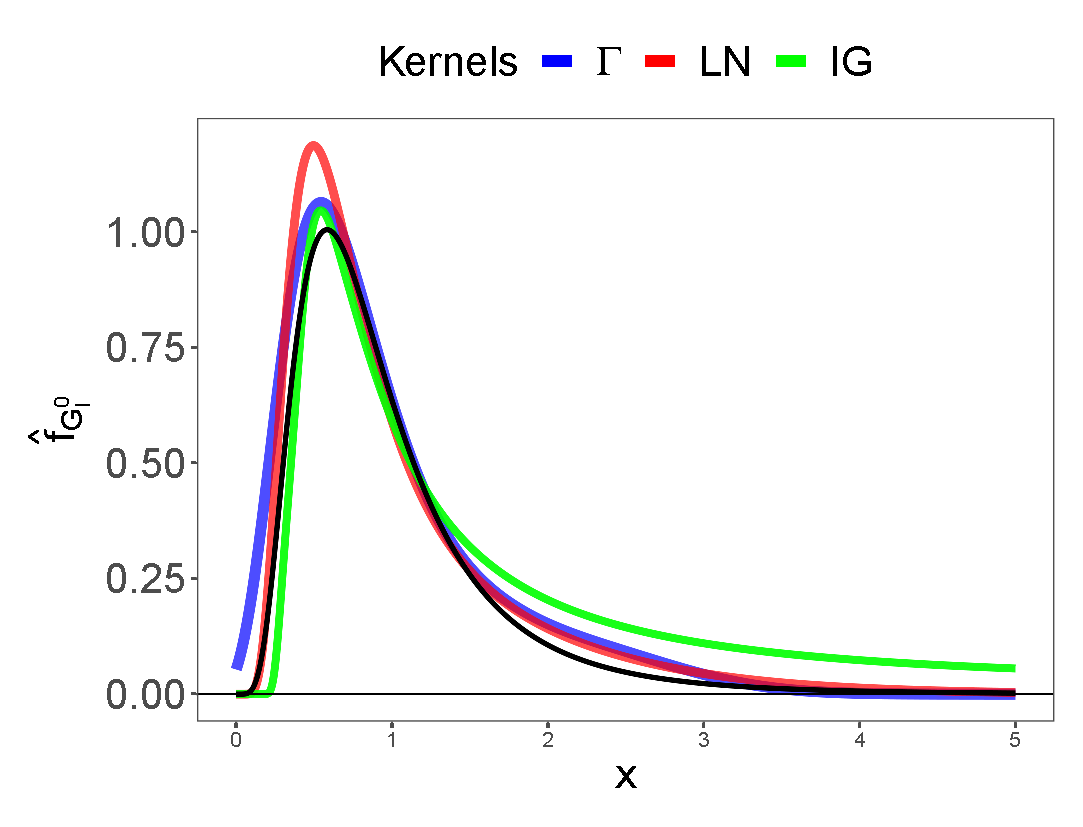
\includegraphics[scale=0.35]{../../../Figures/PaperTesis/NucleosGALNyIG.eps}
	\caption{\label{EstimacionLNyGAyIG} $\widehat{f}_{\mathcal{G}^0}$ for $L=8$, $\alpha=-5$, $\gamma=4$ and $n=25$ using $\Gamma$, LN, and IG kernels, and LSCV for bandwidth selection.}
\end{figure}

It is important to have measures that inform about the quality of the estimation. 
We used the Integrated Mean Square Error (MISE) because it measures the average behavior of the estimator on different samples. 
It is defined as
\begin{align}
\label{Mise}
\text{MISE}(\widehat{f}_b(Z_1,\ldots,Z_n))=&E\left[\int_\mathbb{R} (\widehat{f}_b(z,Z_1,\ldots,Z_n)-f(z))^2 \right].
\end{align}

It is important to note that these kernel estimators are free of boundary bias and achieve the convergence rate $n^{-4/5}$ for the MISE.

%%%%%%%%%%%%%%%%%%%%%%%%%%%%%%%%%%%%%%%%%%%%%%%%%%%%%%%%
%\begin{comment}

%	As known, a measure of the error in the estimation of $f$ by $\widehat{f}$ by the Integrated Squared Error (ISE)
%	\begin{align}
%	\text{ISE}(b)=&\int_\mathbb{R} (\widehat{f}-f)^2 dx = \int_\mathbb{R} \widehat{f}^2dx- 2 \int_\mathbb{R} \widehat{f} fdx +\int_\mathbb{R} f^2dx
%	\label{ISE}
%	\end{align}
%	The last term in this equation does not depend on $b$. 
%	Then
%	\begin{align}
%	\min_b \text{ISE}(b)= \min_b \int_\mathbb{R} \widehat{f}^2 dx- 2 \int_\mathbb{R} \widehat{f} fdx 
%	\label{fi0}
%	\end{align}
%	
%	The second term of equation (~\ref{fi0}) can be seen as $E_X(\widehat{f}(x))$ with $X \sim f$ unknown. The propose is estimate $E_X(\widehat{f}(x))$ by 
%	$$\widehat{E}_{\text{\tiny{X}}}(\widehat{f}(x))=\frac{1}{n}\sum_{i=1}^n \widehat{f}_{-i}(X_i)$$
%	where $\widehat{f}_{-i}(x)= \widehat{f}_{i;b}(x)=\dfrac{1}{n} \displaystyle{\sum_{j=1,j\neq i}^n} K_{(x,b)}(X_i)$, is the leave-one out estimator, the kernel estimator without considering the $i^{th}$ observation.
%	So, the LSCV bandwidth $(b_{\text{LSCV}})$ 
%	%\end{comment}
%	%%%%%%%%%%%%%%%%%%%%%%%%%%%%%%%%%%%%%%%%%%%%%%%%%%%
%	It is defined as:
%	\begin{align}
%	b_{\text{\tiny{LSCV}}}= \arg\min_b \int_\mathbbm{R} \widehat{f}^2 - \frac{2}{n} \sum_{i=1}^n \widehat{f}_{-i}(Z_i)  ,
%	\label{fi}
%	\end{align}
%	where 
%	$$
%	\widehat{f}_{-i}(x)= \widehat{f}_{i;b}(x)=\frac{1}{n} \displaystyle{\sum_{j=1,j\neq i}^n} K_{(x,b)}(Z_i)$$ 
%	is the leave-one out estimator, i.e., the kernel estimator without considering the $i$th observation.
%	If the function to be minimized has more than one minimum, $b_{\text{\tiny{LSCV}}}$ is the largest~\cite{Jones1996}.
%	
%	\subsection{Stochastic Distances Minimization}
%	\label{distance_minimization}
%	
%	It should be noted that one of the points of interest in this work is to find a texture parameter estimator of the $\mathcal{G}^0$ distribution, which behaves well for small sample sizes. 
%	This aspect is interesting because many methods of image filtering or edge detection use sliding masks to estimate parameters. 
%	These mask are usually of size $3 \times 3$, $5 \times 5$, $7 \times 7$, $9 \times 9$ and $11 \times 11$. In this sense, it is known that the MLE estimator dose not present a good behavior when sample size
%	is small. For this reason, it is necessary to find estimators that
%	have asymptotic behavior similar to MLE and outperform the latter for small sample sizes and deviations from the theoretical model.
%	It should be noted that the $\gamma$ parameter of the $\mathcal{G}I^0$ distribution is a scale one. So, to make the results comparable, in the following, we choose the scale parameter such that $E(Z) = 1$, which is given by
%	$\gamma^*= -\alpha-1$.
%	
%	With these tools an using the proposal in~\cite{gambini2015}, we define the estimator of the $\alpha$ parameter of the $\mathcal{G}^0$ distribution based on the minimization of the Triangular stochastic distance using kernel $K$ as :
%	\begin{align}
%	\widehat{\alpha}_{\text{\tiny{K}}}= \arg\min_{\alpha} d_{\text{\tiny{T}}}\big(f_{\mathcal{G}^{0}}(\alpha,\gamma^*, L ), \widehat f_{\text{\tiny{K}}}(z)\big),
%	\label{minimization}
%	\end{align}
%	where $d_{\text{T}}$ is the triangular distance defined in~\eqref{DT}, $\gamma^*$ and $L$ are known, and $\widehat f_{\text{\tiny{K}}}(z)$ is a nonparametric estimation of the underlying density function using kernel $K$. 
%	
%	Figure~\ref{densidades} shows the graph of the $\mathcal{G}^0$ density function for  $\alpha=\{-20,-25\}$, $\gamma=\gamma^*$, $L=\{3,8\}$. It can be seen that these densities are very similar since the $\mathcal{G}^0$ converges in distribution to a $\Gamma(L,L)$~\cite{Frery99} when  $\alpha \longrightarrow -\infty$ and $\gamma=\gamma^*$. For this reason it is proposed that $\alpha$ take values in the range $[-20,-1]$. 
%	
%	\begin{figure}[hbt]
%		\centering
%		\subfigure[L=3]{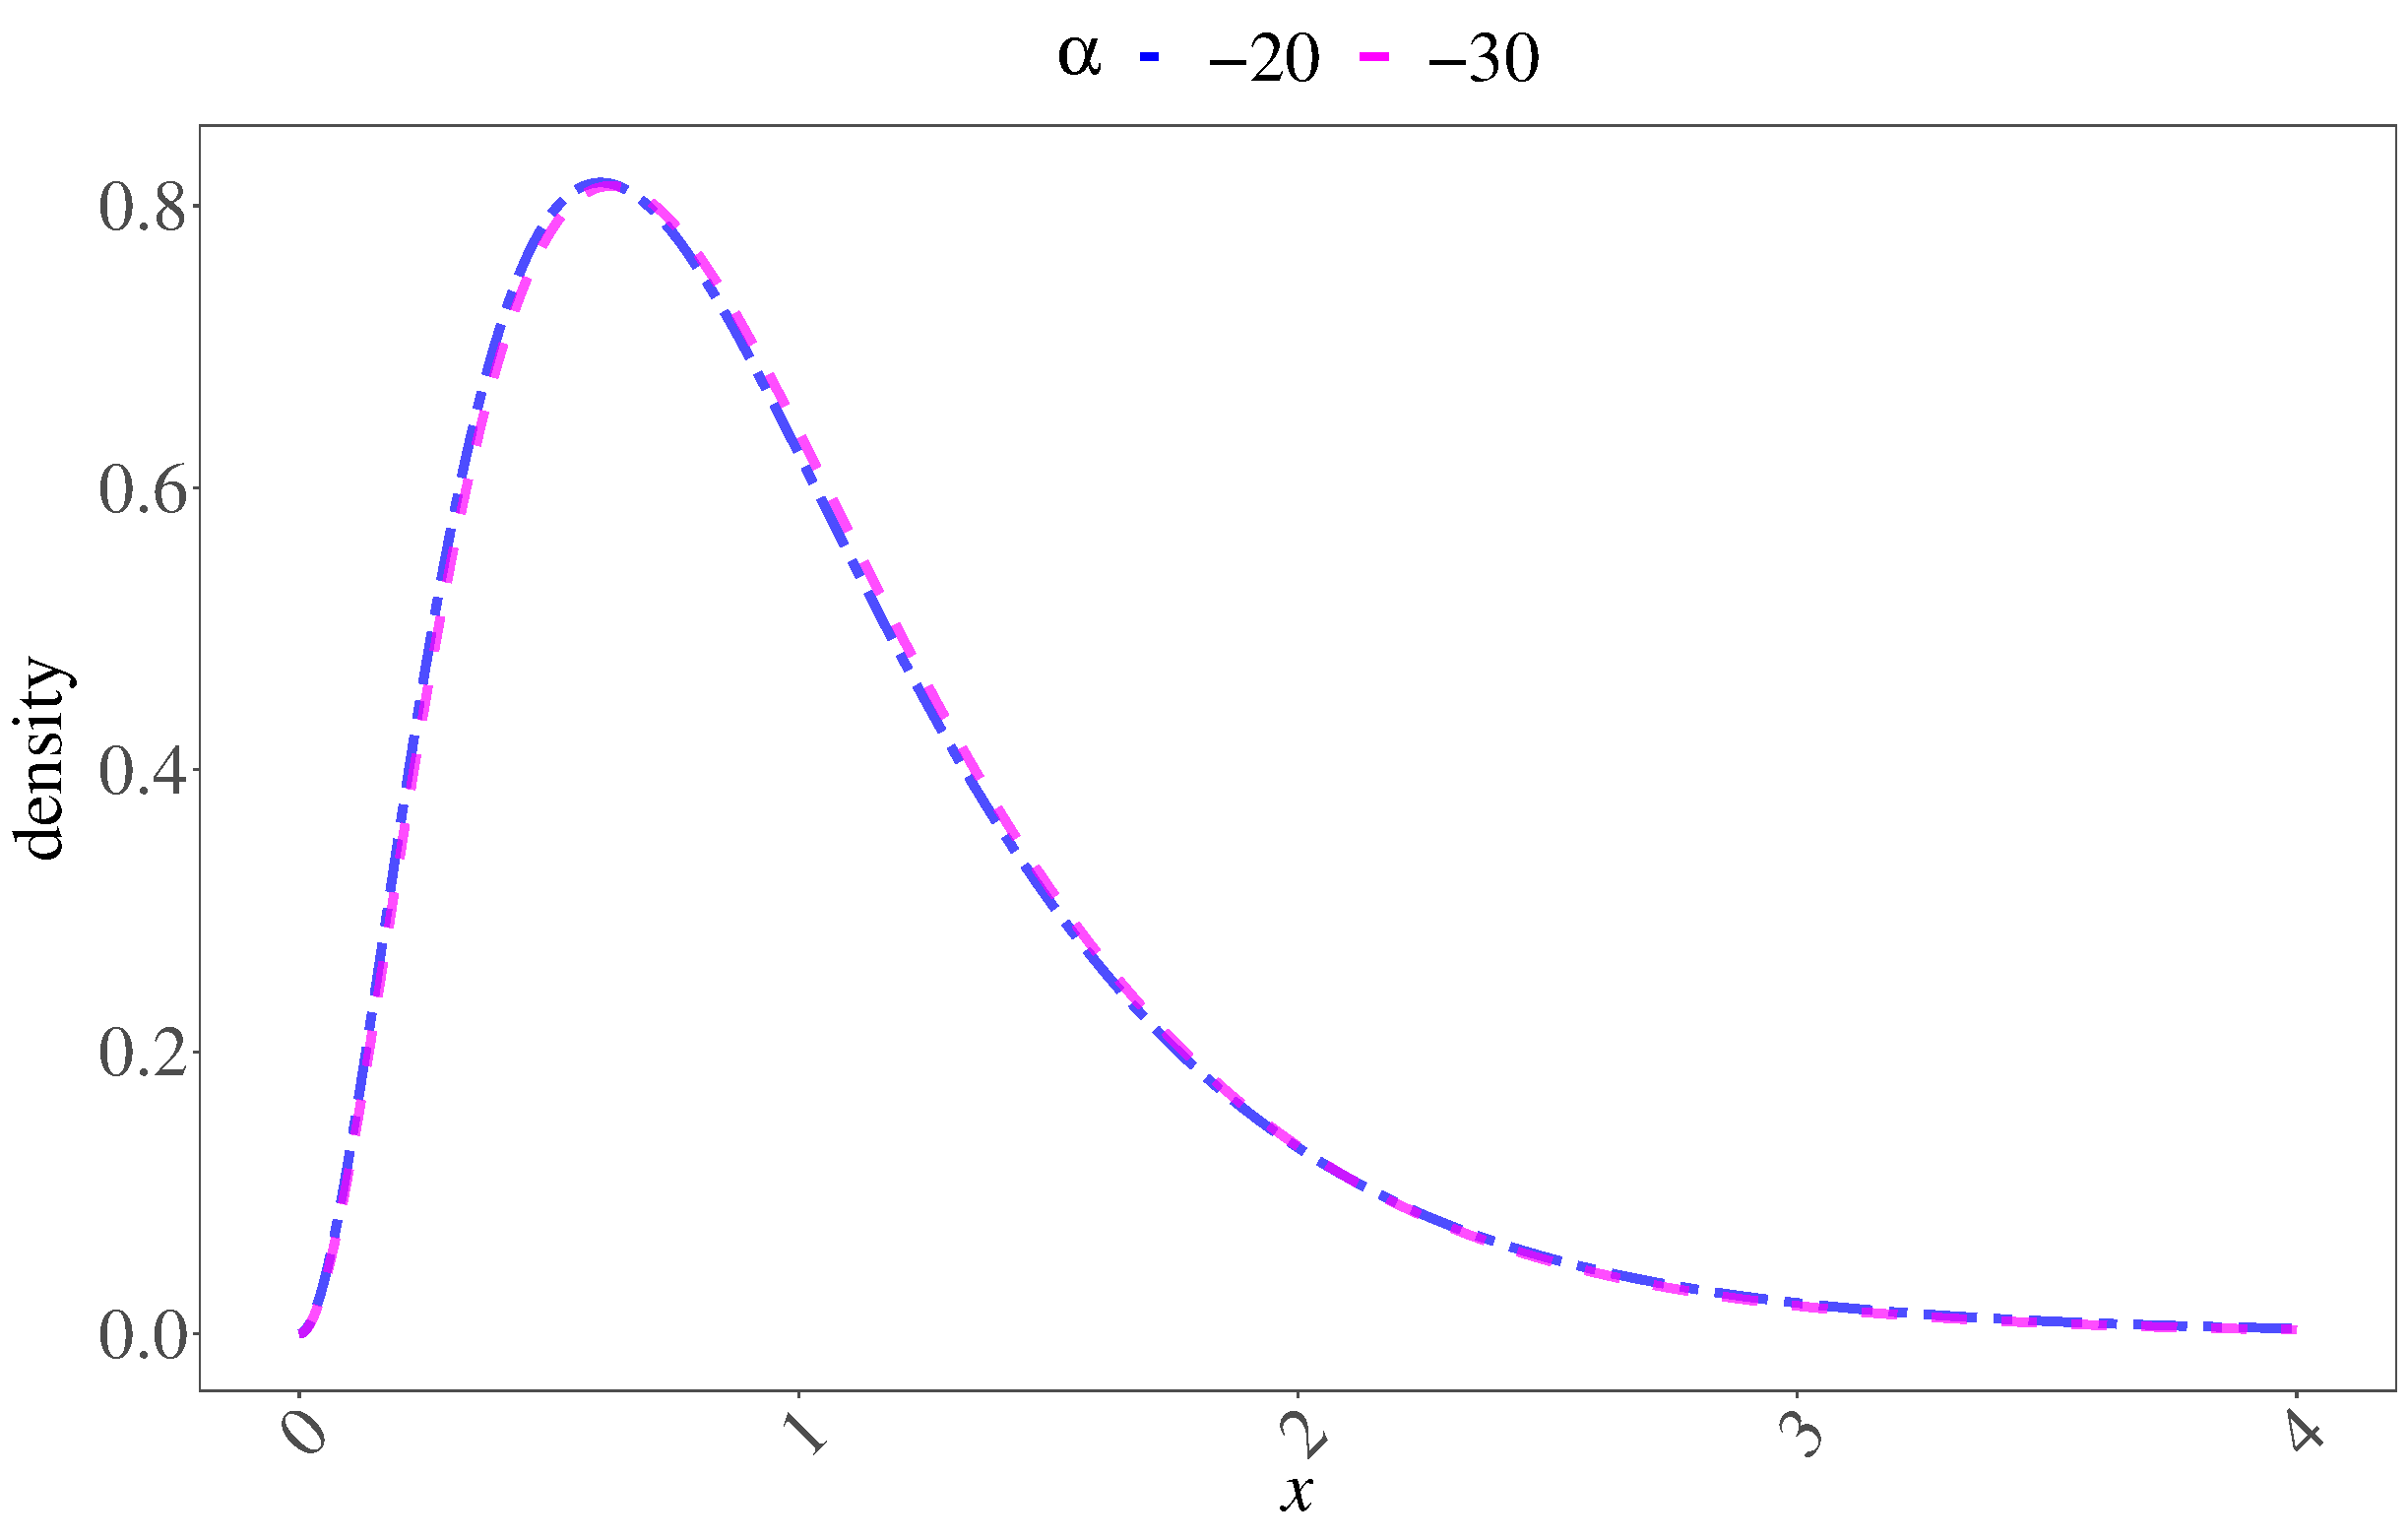
\includegraphics[width=.45\linewidth]{../../../Figures/PaperTesis/DensidadGI0L3}}
%		\subfigure[L=8]{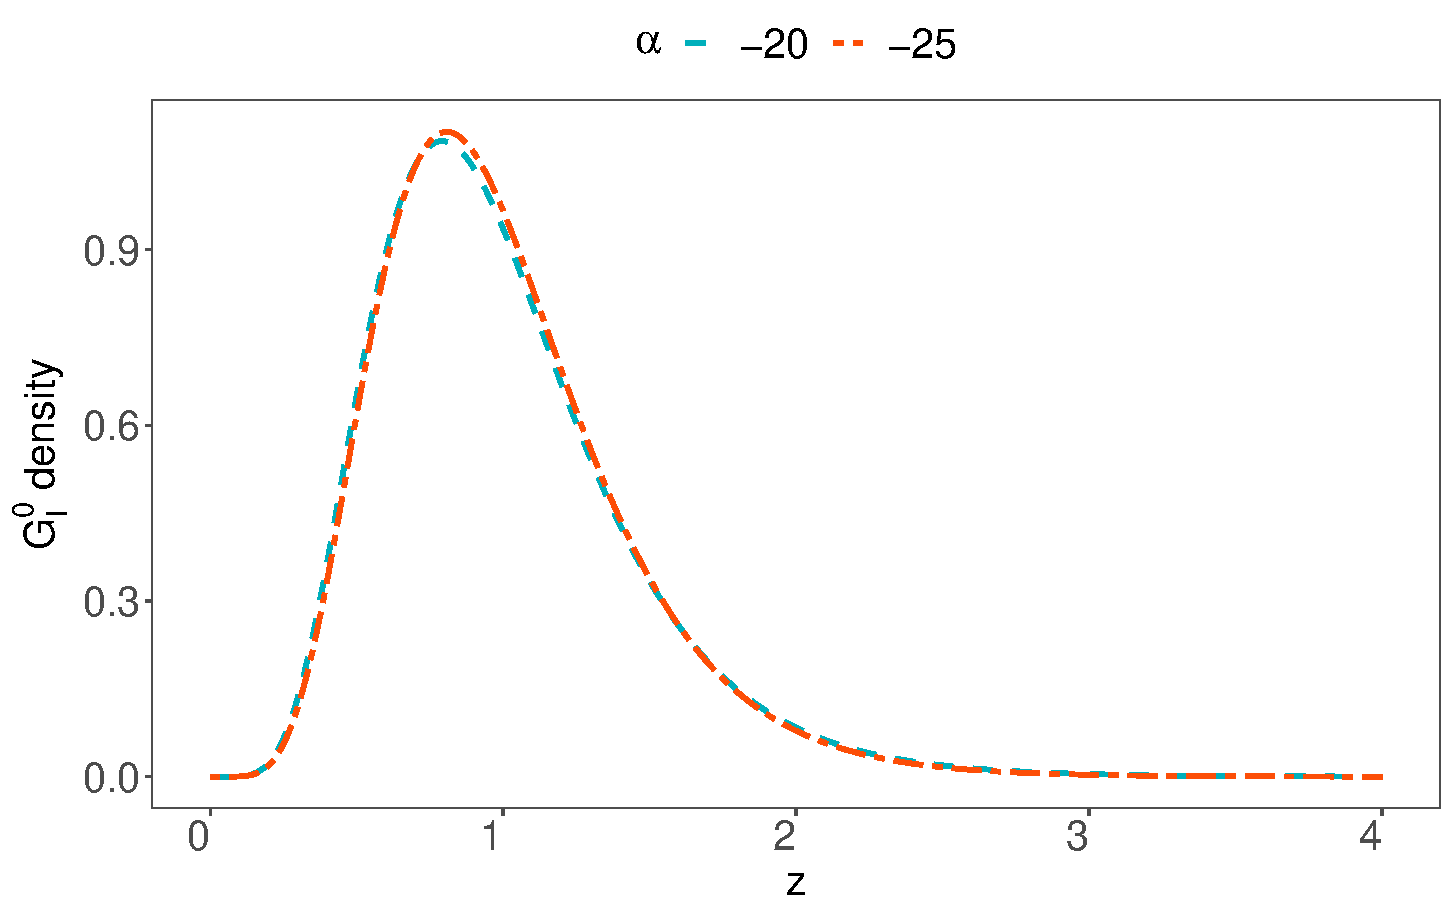
\includegraphics[width=.45\linewidth]{../../../Figures/PaperTesis/DensidadGI0L8}}
%		\caption{\label{densidades} $\mathcal{G}^0(\alpha,\gamma^*,L)$ densities}
%	\end{figure}


%This minimization was performed searching values in $[-20,-1]$ and returning as $\widehat{\alpha}_{\text{\tiny{K}}}$ the value that minimizes~\eqref{minimization}.
%As it is mentioned in section~\ref{sec_SAR}, the parameter $\gamma_0$ is chosen such that the expected value of the return $Z$ is one. This condition leads to the following relation: $\gamma_0^*=-\alpha-1$.

\subsection{Logcumulant estimator}\label{lc}

%%% ACF This paragraph is not clear
It is known the relationship between the random variable moments and its characteristic function, defines as the Fourier transform of its probability density function (pdf). 
Using this approach, we define moment estimators. 

In the same sense, Nicolas et al.~\cite{nicolas2002} defined the first characteristic function of the second kind as the Mellin transform of its pdf function for the case where the density function has positive support. 

Gambini et al.~\cite{gambini2015} show that the LC estimator for the $\alpha$ parameter of the $\mathcal{G}^0$ distribution, under the relationship~\eqref{RelationAlphaGamma}, is the solution of 
\begin{equation} \label{eq:logm}
\frac{1}{n} \sum_{i=1}^n\log z_i =   -\log \frac{L}{-\widehat\alpha_{\text{{LC}}}-1} + \Psi^0(L) - \Psi^0(-\widehat\alpha_{\text{{LC}}}).
\end{equation}
The right term of the equation~\eqref{eq:logm} is a monotone decreasing function of $\alpha$. Therefore, this equation has a single root or none. 
This estimator is widely used in SAR image processing. 
Refs~\cite{MellinAnalysisPolSAR,BujorTrouveValetNicolas2004,khan2014} applied this methodology due to its nice properties and good performance. 
More recently, Nogueira et al.~\cite{Nogueira2019} used the LC estimator applied in an unsupervised algorithm for SAR image segmentation.

We compare our proposal with LC and ML estimators because these are widely used in the literature.

%	 From this, if $X \sim f_{\text{\tiny{X}}}(u)$ it can be defined:
%	\begin{itemize}
%		\item First characteristic function of second kind:  
%		\begin{align*}
%		\phi_{\text{\tiny{X}}}(s) = \int_0^{\infty} u^{s-1}f_{\text{\tiny{X}}} (u)du.
%		\end{align*}
%		\item Second characteristic function of second kind: 
%		\begin{align*}
%		\psi_{\text{\tiny{X}}}(s) = \log\phi_{\text{\tiny{X}}}(s).
%		\end{align*}
%		\item Second kind characteristic moment:
%		\begin{align*}
%		\tilde{m}_r = \frac{d \phi_{\text{\tiny{X}}}(s)}{ds } \at[\Big]{s=1}. \label{eq:fcm}
%		\end{align*}
%		\item Second kind characteristic cumulant (Logcumulant)
%		\begin{equation}
%		\tilde{k}_r = \frac{d \psi_{\text{\tiny{X}}}(s)}{ds} \at[\Big]{s=1}. \label{eq:scm}
%		\end{equation}
%	\end{itemize}


%	If $f_x(u) = \mathcal{G}^0(u)$ then we have:
%		\begin{align*}
%		\phi_x(s) = \frac{\left(\frac{L}{\gamma}\right)^{1-s}\Gamma(-1+L+s)\Gamma(1-s-\alpha)}{\Gamma(L)\Gamma(-\alpha)}
%		\end{align*}
%		\begin{align}
%		\widetilde{m}_1 =  \frac{d \phi_x(s)}{ds } \at[\big]{s=1} = -\log(\frac{L}{\gamma}) + \Psi^0(L) - \Psi^0(-\alpha).
%		\end{align}
%	
%	According to~\cite{Tison2004}, we have that $\widetilde{k}_1 = \widetilde{m_1}$, then
%	\begin{align}
%	\widetilde{k}_1 =   -\log \frac{L}{\gamma} + \Psi^0(L) - \Psi^0(-\alpha). \label{eq:scGi}
%	\end{align}
%	
%	 and the empirical expression for the first logcumulant for a sample $Z_1,\ldots,Z_n$ is $\widehat{\widetilde{k}}_1 ={n}^{-1} \sum_{i=1}^n\log Z_i$. Therefore this relationship can be used to estimate the parameters of the distribution. 

%	
%	As was mentioned in section \ref{sec_SAR} we assume that $\gamma^*=-\alpha-1$, then the Log-cumulant estimator of $\alpha$, denoted by $\widehat\alpha_{\text{{LC}}}$ is then the solution of 
%	$\widehat{\widetilde{k}}_1 =   -\log \frac{L}{-\widehat\alpha_{\text{{LC}}}-1} + \Psi^0(L) - \Psi^0(-\widehat\alpha_{\text{{LC}}})$, that is, 

\subsection{Robustness analysis -- Stylized Samples}
\label{robustez}
Among the desirable properties of a good estimator, resistance to contamination is very important in practical applications. 
That is, its ability to produce good estimations even when a proportion of the data does not come from the assumed model. 
This situation is of particular importance in the case of small sample sizes, e.g., when using filters defined on sliding windows of size $3 \times 3$, $5 \times 5$ or, for instance, $7 \times 7$. 
These windows may contain data from areas with different textures, for example, at the edges between different regions or corner reflectors (features that produce a few very large observations with respect to the background).

In image processing and analysis, it is difficult to grant the underlying hypothesis under which the techniques being employed hold, so the ability to perform well even under deviations from these assumptions is a requirement.

In order to assess the robustness of the proposed estimators we consider different alternatives. 
The first one is to consider that, in a small proportion $\epsilon$, the data may suffer deviations of the theoretical model. 
In this case we define random variables $W \sim \mathcal{G}^0(\alpha_1,\gamma_1^*,L)$ and $U \sim \mathcal{G}^0(\alpha_2,\gamma_2^*,L)$, where $\gamma_1^*=-\alpha_1-1$ and  $\gamma_2^*=-\alpha_2-1$. 
We consider the Bernoulli random variable $B$ with a probability of success $\epsilon$ indicating the contamination ratio.   
We define $Z=BU+(1-B)W$ by its cumulative distribution function   
$
\epsilon {F}_{\alpha_2,\gamma_2^*,L}(z)+(1-\epsilon) {F}_{\alpha_1,\gamma_1^*,L}(z)
$.
This schema considers that, in average, a small proportion $\epsilon$ of the data come from the same family but with different parameters. 

%%% ACF Was this contamination model used in this work?
Sometimes certain pixels present an extremely high return value. 
This phenomenon is produced by double bounce or by a corner reflector, and is one of the sources of contamination in SAR imagery. 
The presence of such outliers may provoke big errors in the estimation as we show in an application to a real image. 

A way of assessing how the estimator $T_n(z_1,\dots,z_n)$ behaves under contamination is by fixing $n-1$ observations and allowing one to vary.
This is the EIF -- Empirical Influence Function, but it depends on the particular sample.
To avoid this, Andrews et al.~\cite{Andrews1972}, proposed using the $i^{th}$ quantile of the assumed distribution as typical observations: $z_i=F^{-1}\big((i-1/3)/(n+1/3) \big)$, $1\leq i\leq n-1$.
This is the SEIF -- Stylized Empirical Influence Function that, among others, was used by Rousseeuw and Verboven~\cite{RousseeuwCSDA} for estimation with very small samples and by Allende et al.~\cite{AllendeFreryetal:JSCS:05} for AM estimators of the texture under the amplitude $\mathcal G^0$ law.

The quantiles of a $\mathcal G^0(\alpha,\gamma,L)$ random variable can be obtained by $\Upsilon^{-1}_{2L,-2\alpha}$, the inverse of~\eqref{eq:CDFG0}, also available in most statistical computing environments.


\section{Performance Analysis}\label{simulation}

This section presents empirical results about the quality of estimators for the texture parameter under the $\mathcal G^0$ distribution. 
We will consider that an algorithm converges if it finds an estimate for $\alpha$ in the interval $[-20,-1]$.	

Figure~\ref{densidades} shows the $\mathcal{G}^0$ densities for  $\alpha=\{-20,-25\}$, $\gamma=\gamma^*$, and $L=\{3,8\}$. 
These densities are very similar since the $\mathcal{G}^0$ law converges in distribution to the $\Gamma(L,L)$ law when $\alpha \to -\infty$ and $\gamma=\gamma^*$~\cite{Frery99}. 
For this reason, our approach assumes that $\alpha$ takes values in the range $[-20,-1]$. 

\begin{figure}[htb]
	\centering
	\subfigure[$L=3$]{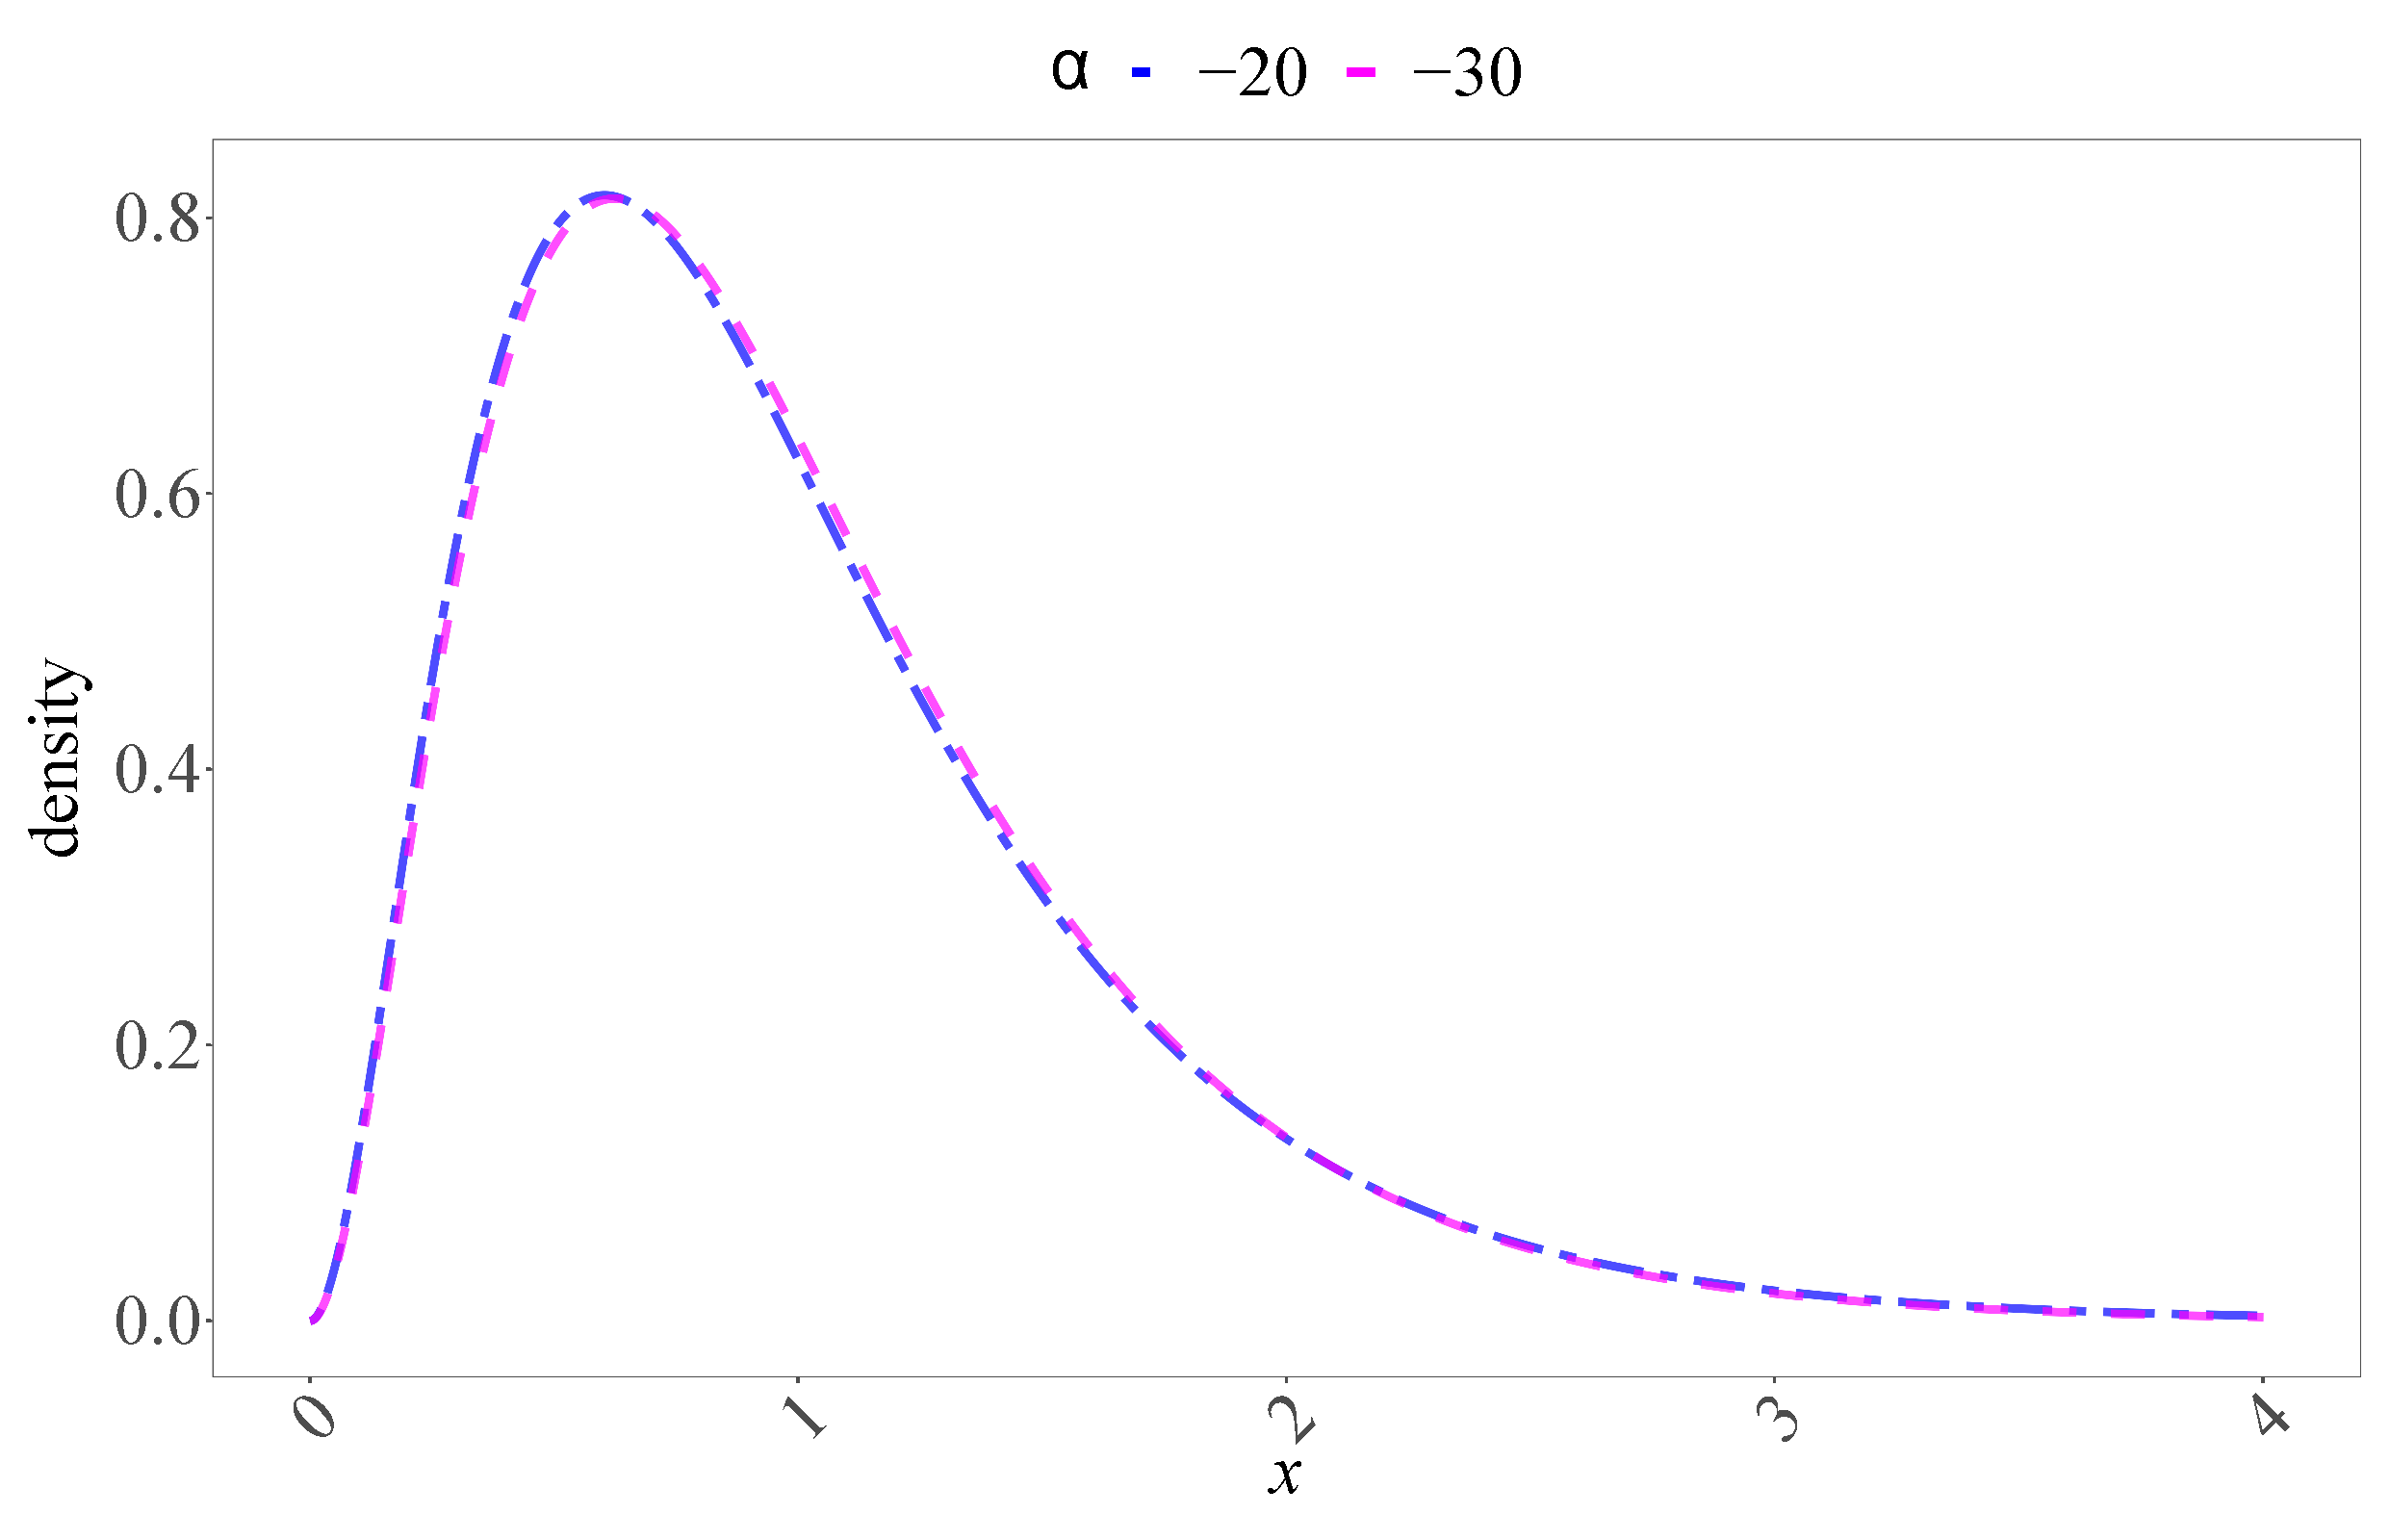
\includegraphics[width=.75\linewidth]{../../../Figures/PaperTesis/DensidadGI0L3.eps}}
	\subfigure[$L=8$]{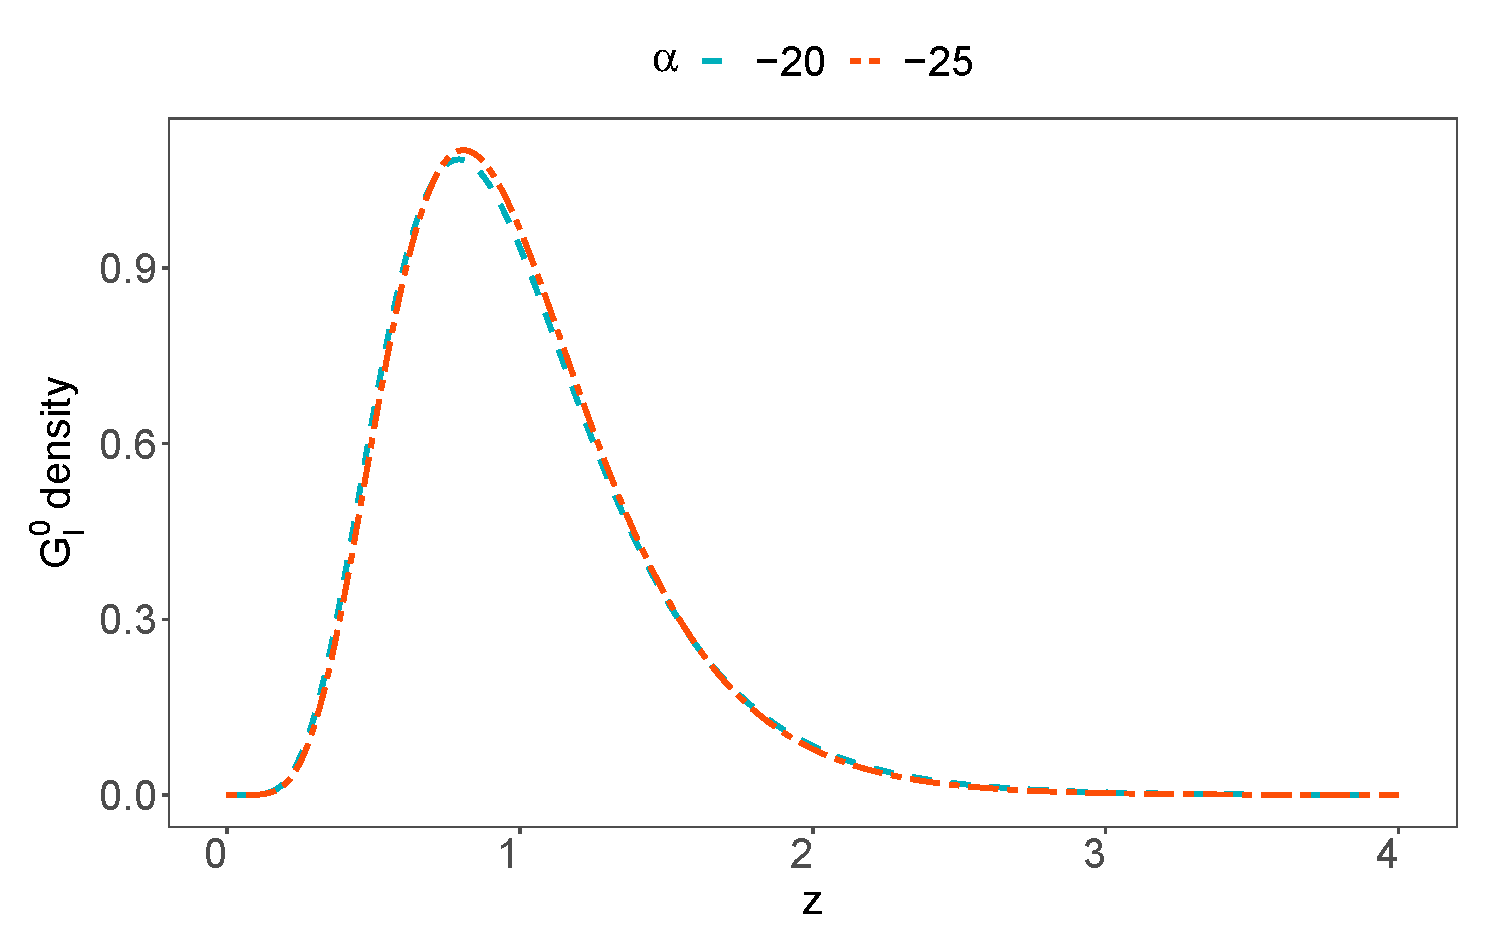
\includegraphics[width=.75\linewidth]{../../../Figures/PaperTesis/DensidadGI0L8.eps}}
	\caption{\label{densidades} $\mathcal{G}^0(\alpha,\gamma^*,L)$ densities.}
\end{figure}

Many methods of image filtering and edge detection use sliding masks to estimate parameters. 
These mask are usually of size $3 \times 3$, $5 \times 5$, $7 \times 7$, $9 \times 9$ and $11 \times 11$. 
For this reason, we chose $n=9,25,49,81,121$ as sample size to perform the empirical analysis.

%	It should be noted that it is of interest to find a texture parameter estimator which behaves well for small sample sizes. This aspect is interesting because many methods of image filtering or edge detection use sliding masks to estimate parameters. These mask are usually of size $3 \times 3$, $5 \times 5$, $7 \times 7$, $9 \times 9$ and $11 \times 11$.
%	
First of all, we evaluate the performance of the $\Gamma$, LN, and IG kernels studying MISE and the percentage of non-convergence cases, in order to choose the kernel that produces the best fits of the data. 
We use the LSCV method to find the bandwidth, and, for IG kernel, we also review the empirical bandwidth ($\text{IG}_{\text{E}}$) studied in Ref.~\cite{gambini2015}. 

Table~\ref{pp} shows the values of $\widehat{\text{MISE}}$ and non-convergence percent. 
It can be seen that IG and $\text{IG}_{\text{E}}$ present MISE values of several orders of magnitude greater than the other kernels. 
The same happens for non-convergence cases. 
The IG kernel has the highest percentage of these cases compared to the $\Gamma$ and LN kernel.

\begin{table}[hbt]  
	\caption{\label{pp} Estimated MISE and percentage of non-convergence cases for $L=3$.}        
	\centering                                    
	\begin{tabular}{cc S[table-format=0.1]S[table-format=0.1]S[table-format=0.1] S[table-format=0.1] @{\hskip 8mm} S[table-format=0.2]S[table-format=0.1]S[table-format=0.1]S[table-format=0.1]}                                    
		\toprule                                    
		\multirow{4 }{3mm}{$\alpha$} &\multirow{4 }{*}{ $n$  } & \multicolumn{4}{c}{\multirow{2 }{*}{$\widehat{\text{MISE}}$}} & \multicolumn{4}{c}{\centering \% }\\
	 &                          &                &               &         &     &   \multicolumn{4}{c}{non convergence cases}\\
		
		\cmidrule(r){3-6}
		\cmidrule(r){7-10}
		%\midrule
		
		&           & \mc{$\Gamma$} & \mc{LN}       & \mc{IG}     & \mc{$\text{IG}_{\text{E}}$}    & \mc{$\widehat{\alpha}_{\Gamma}$} & \mc{$\widehat{\alpha}_{\text{{LN}}}$}    & \mc{$\widehat{\alpha}_{\text{\tiny{IG}}}$} & \mc{$\widehat{\alpha}_{\text{\tiny{IG}}_{\text{E}}}$}\\
		\midrule                
		\multirow{5 }{3mm}{$-1.5$} 
		&  9       &       0.41     &     0.81     &     6.12      &     41.33     &    0     &    0.4      &    0.4       &    0 \\        
		&  25      &       0.12     &     0.18     &     2.46      &     17.02     &    0     &    0        &    0        &    0 \\
		&  49      &       0.08     &     0.54     &     1.16      &      9.67     &    0     &    0        &    0        &    0 \\
		&  81      &       0.06     &     0.08     &     0.75      &     6.13      &    0     &    0        &    0        &    0 \\
		&  121     &       0.06     &     0.08     &     0.53      &     4.00      &    0     &    0        &    0        &    0 \\
		\midrule                                    
		\multirow{5 }{3mm}{$-3$}    
		&  9       &       0.25     &     0.56     &     12.48     &     50.02     &    5.2    &    7.2     &   8         & 6.8 \\                    
		&  25      &       0.08     &     0.11     &     3.22      &     25.40     &    0.2    &    1       &    0.6      & 0.6 \\        
		&  49      &       0.04     &     0.07     &     0.69      &     16.40     &    0      &    0.4     &    0        &    0 \\
		&  81      &       0.03     &     0.03     &     0.25      &     11.58     &    0      &    0       &    0        &    0 \\
		&  121     &       0.02     &     0.03     &     0.17      &     8.98      &    0      &    0       &    0        &    0 \\    
		
		\midrule                                        
		\multirow{5 }{3mm}{$-5$}    
		&  9       &       0.24     &     0.43     &     15.32     &     63.38     &    9.6    &    13.2    &   17         &    13.2 \\                    
		&  25      &       0.07     &     0.09     &     4.65      &     32.94     &    3.4    &   5        &    2         &    1.6 \\                    
		&  49      &       0.04     &     0.06     &     0.68      &     24.41     &    1.4    &    1.2     &    1         &    0.4 \\
		&  81      &       0.03     &     0.03     &     0.29      &     18.91     &    0.4    &    0.8     &    0.2       &    0 \\
		&  121     &       0.02     &     0.02     &     0.18      &     15.92     &    0      &    0.2     &    0         &    0 \\
		
		\midrule                                        
		\multirow{5 }{3mm}{$-8$}    
		&  9       &       0.24     &     0.38     &     18.11     &     73.08     &    16.6    &    19     & 26.2         &    18 \\                
		&  25      &       0.07     &     0.11     &     5.13      &     40.48     &    81.8    &   11      &    8.8       &    4.2 \\            
		&  49      &       0.04     &     0.05     &     0.93      &     30.23     &    5       &    5.4    &    4.2       &    1.2 \\    
		&  81      &       0.03     &     0.03     &     0.33      &     25.71     &    4.4     &    4      &    2         &    0.2 \\    
		&  121     &       0.02     &     0.02     &     0.21      &     21.19     &    1.8     &    2      &    0.8       &    0.4 \\
		\bottomrule
	\end{tabular}                                              
\end{table}    

Therefore, we chose $\Gamma$ and LN kernels to estimate the underlying density function.

The following analysis was performed through a Monte Carlo experiment, which consists of $500$ independent replications for each of several parameter values: 
$L\in\{3,8\}$ to consider multilook case,
$\alpha\in\{-1.5, -3, -5, -8\}$ to represent different levels of texture, 
and 
$n\in\{9, 25,49, 81,121,500\}$ to consider different scenarios of window sizes, and a large sample situation.

Each replication produces estimates $\{\widehat{\alpha}_1, \dots, \widehat{\alpha}_{500}\}$ with which we compute 
the sample mean $\overline{\widehat{\alpha}}=(500)^{-1}{\sum_{i=1}^{500}{\widehat{\alpha}_i}}$, 
the sample bias $\widehat{B}(\widehat\alpha) = \overline{\widehat\alpha}- \alpha$, 
and 
the sample mean squared error $\widehat{\operatorname{mse}}=({500})^{-1}{\sum_{i=1}^{500}{(\widehat{\alpha}_i-\alpha)^2}}$.


We compare four estimators for the multilook case: 
$\widehat{\alpha}_{\text{{ML}}}$, 
$\widehat{\alpha}_{\text{{LC}}}$, 
$\widehat{\alpha}_{\Gamma}$ ($\Gamma$ kernel) and $\widehat{\alpha}_{\text{{LN}}}$ (LN kernel).

The performance of the proposed techniques is assessed twofold: in pure and contamination cases. 
%Through the Monte Carlo experiment, we evaluate the bias and the mean squared error in different stages. 
We also assess the robustness of these estimators by means of their Stylized Empirical Influence Functions (SEIFs) and contaminating the data, as explained in subsection~\ref{robustez}. 
The estimators were also evaluated in terms of the percentage of situations for which there was no convergence, and by their computational cost. 
For $\widehat{\alpha}_{\text{{LN}}}$ we also account, as a case of non-convergence, for situations where no solution was found for equation~\eqref{eq:logm}.


\subsection{Computational Information}

Table~\ref{NoConvMLyNGyLNyLC_L=3} shows the percentage of non-convergence cases for $L=3$; the situation for $L=8$ yields similar values and, thus, is not reported for brevity.
It can be seen that the $\widehat{\alpha}_{\text{{ML}}}$ and $\widehat{\alpha}_{\text{{LC}}}$ estimators have the highest values of lack of convergence followed by  $\widehat{\alpha}_{\text{{LN}}}$ and $\widehat{\alpha}_{\Gamma}$.

\begin{table}[hbt]
	\caption{Percentage of non-convergence cases,  $L=3$.}
	\centering
	\label{NoConvMLyNGyLNyLC_L=3}
	\begin{tabular}{c*6{r}}
		\toprule        
		$\alpha$ & $n$ & $\widehat{\alpha}_{\text{{ML}}}$ & $\widehat{\alpha}_{\Gamma}$ & $\widehat{\alpha}_{\text{{LN}}}$ &  $\widehat{\alpha}_{\text{{LC}}}$\\
		\midrule
		\multirow{2 }{*}{$-1.5$} 
		&   $9$ & $0$ & $0$ & $0.4$ &  $2.8$\\
		&  $25$ & $0$ & $0$ & $0$ & $0.2$\\
		\midrule
		\multirow{5 }{*}{$-3$} 
		&   $9$ & $13$    & $5.2$  & $7.2$  &  $28.4$\\ 
		&  $25$ & $1$     & $0.2$  & $1$    &  $11.4$\\
		&  $49$ & $0.2$   & $0$    & $0.4$  & $3.8$\\ 
		&  $81$ & $0$     & $0$    & $0$    & $2.4$\\ 
		& $121$ & $0$     & $0$    & $0$    & $0.2$\\ 
		\midrule
		\multirow{5 }{*}{$-5$} 
		&   $9$ & $26.8$  & $9.6$  & $13.2$ &  $35.2$\\ 
		&  $25$ & $10$    & $3.4$  & $5$    & $28.6$\\ 
		&  $49$ & $3.4$   & $1.4$  & $1.2$  & $18.6$\\ 
		&  $81$ & $0.2$   & $0.4$  & $0.8$  & $15.8$\\ 
		& $121$ & $0.4$   & $0$    & $0.2$  & $9.6$\\ 
		& $500$ & $0$     & $0$    & $0$    & $0.6$\\ 
		\midrule
		\multirow{5 }{*}{$-8$} 
		&   $9$  & $39.6$ & $16.6$ & $19$   & $44.2$\\ 
		&  $25$  & $28.6$ & $9$    & $11$   & $36.4$\\ 
		&  $49$  & $18.4$ & $5$    & $5.4$  & $31.6$\\ 
		&  $81$  & $12$   & $4.4$  & $4$    & $27.2$\\ 
		& $121$  & $5.8$  & $1.8$  & $2$    & $24.6$\\ 
		& $500$  & $0$    & $0$    & $0.2$  & $9$\\
		\bottomrule     
	\end{tabular}
\end{table}    

Moreover, such lack of convergence is more pronounced for homogeneous ($\alpha=-8$) and textured ($\alpha=-5$) areas. 
This issue had been observed for amplitude data in~\cite{FreryCribariSouza:JASP:04} for $\widehat{\alpha}_{\text{{ML}}}$, and is related to the decreasing curvature of the likelihood function.

Table~\ref{tablaDeTiemposmediosMLyGAyLNyLC} shows the mean system time, in seconds, for five hundred replications for each estimator, considering $\alpha=-5$ and sample $n=81$. 
Albeit $\widehat{\alpha}_{\Gamma}$ and $\widehat{\alpha}_{\text{{LN}}}$ require much more processing time than the others estimators, the former fail to converge about half of the times that the last.
%%% ACF Mean system time is not that relevant at this point, and requires informing the platform (processor, operating system, programming language, libraries etc.) It is much more informative to provide relative values to the fastest technique and, in an appendix, provide that information and the meaning of the reference value

\begin{table}[hbt]
	\caption{Mean system time for uncontaminated data, $L=3$ and $n=81$. }
	\label{tablaDeTiemposmediosMLyGAyLNyLC}
	\centering
	\begin{tabular}{cccc}
		\toprule
		ML& $\Gamma$ & LN & LC \\
		\cmidrule(lr){1-4}
		$0.003$& $1.87$ & $1.87$ &$0.003$ \\
		\bottomrule
	\end{tabular}
	
\end{table}

\subsection{Simulation Results -- Pure Cases}

Figure~\ref{SesgoyECMSinContL=3} shows the bias and mean square error (MSE) for uncontaminated data, $L=3$, and varying sample size. 
The results are shown in semilogarithm scale. 
The iterations considered are those where all methods converge. 

We also plot the confidence interval of approximately \SI{95}{\percent} level for each estimate, using the percentile method described in Ref.~\cite{Buckland1983}. 
This method consists in using the percentile $(\alpha/2)$ and $(1-\alpha/2) $ of the distribution of $\widehat{\alpha}$. 
This method was evaluated by~\cite{Buckland1983} in the case where the underlying distribution is exponential, where the symmetry of the distribution fails. 
The author shows that this interval has a better performance than using the normal approximation. 

It can be seen that, for a fixed $n$ and as $\alpha$ decreases, both  $\widehat{\text{Bias}}$ and $\widehat{\text{MSE}}$ increase in most methods. 
It is important to note that $\widehat{\alpha}_{\text{{ML}}}$ and $\widehat{\alpha}_{\text{{LC}}}$ on the one hand, 
and $\widehat{\alpha}_{\Gamma}$ and $\widehat{\alpha}_{\text{{LN}}}$ on the other hand, have similar behavior in both bias and MSE in most cases. 
This similar behavior can also be observed in the confidence intervals: $\widehat{\alpha}_{\text{{ML}}}$ and $\widehat{\alpha}_{\text{{LC}}}$ produce wider intervals than the other estimators, showing that they are less accurate than MDE.

%%% ACF Add in parentheses the values of \alpha you are referring to for each kind of area
For extremely heterogeneous and heterogeneous areas, the MDE estimators have a better performance than the rest. 
For moderately heterogeneous areas, all methods have similar behavior; however, MDE has lower MSE. 
For homogeneous areas $\widehat{\alpha}_{\text{{ML}}}$ is the one with the smalles bias, although the MSE is comparable to the MDE estimators except for moderate size samples where the MSE is larger.

\begin{figure}[htb]
	\centering
	\subfigure[\label{SesgoSinContL=3}$\widehat{\text{Sesgo}}$]{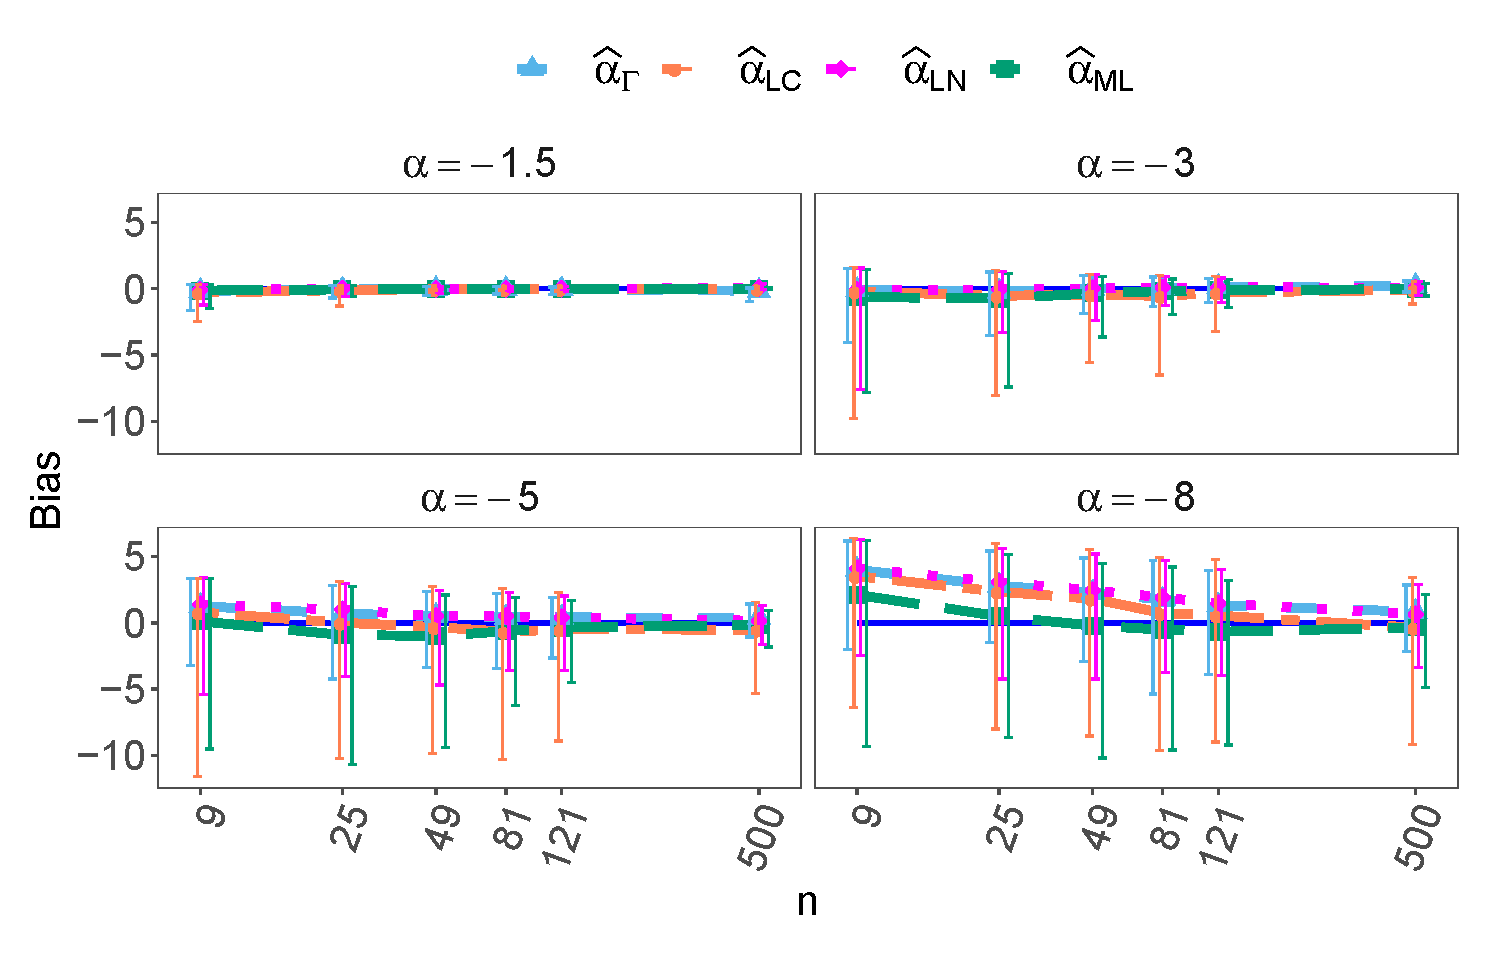
\includegraphics[width=0.9\linewidth]{../../../Figures/PaperTesis/GraficoSesgoMVyGAyLNyLC_L=3SinCont_BarrasErroryPercentil.eps}}
	\subfigure[\label{ECMSinContL=3}$\widehat{\text{MSE}}$]{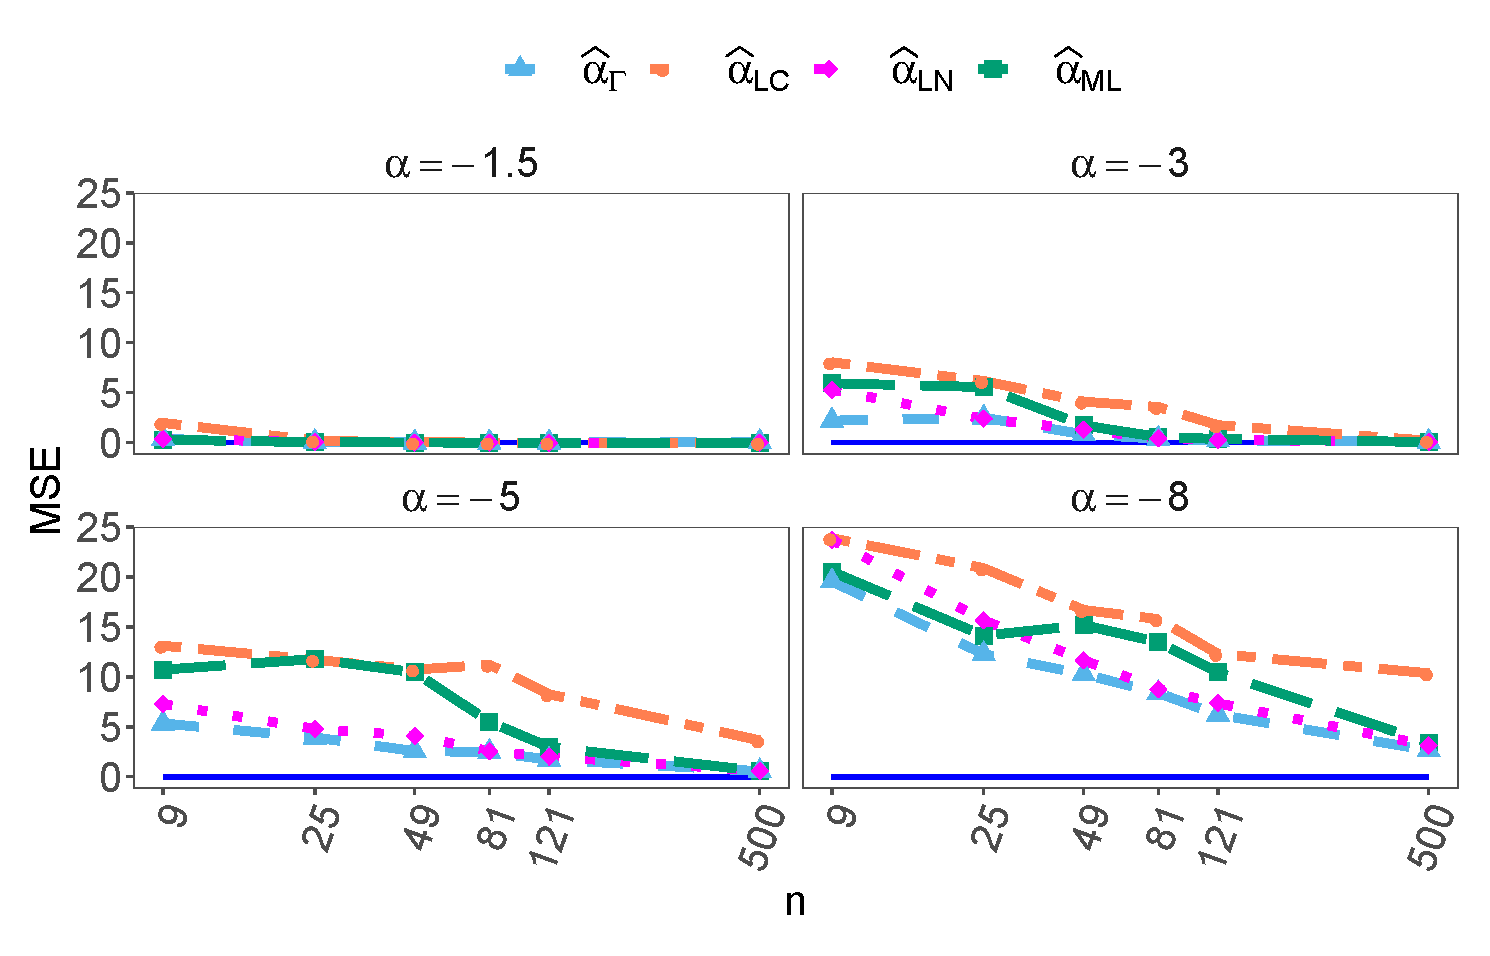
\includegraphics[width=0.9\linewidth]{../../../Figures/PaperTesis/GraficoECMMVyGAyLNyLC_L=3SinCont_BarrasErroryPercentil.eps}}
	\caption{\label{SesgoyECMSinContL=3}\small Sample Bias and MSE with uncontaminated data and $L=3$.}
\end{figure}    

A similar analysis was done for the case $L=8$. Figs.~\ref{SesgoSinContL=8} and~\ref{ECMSinContL=8} show that $\widehat{\alpha}_{\text{{ML}}}$ has the best performance for homogeneous
%%% ACF "exceeds"? 
areas in terms of bias, while $\widehat{\alpha}_{\text{{LN}}}$ exceeds the rest in extremely textured areas with moderate texture.

\begin{figure}[htb]
	\centering
	\subfigure[\label{SesgoSinContL=8}$\widehat{\text{Sesgo}}$]{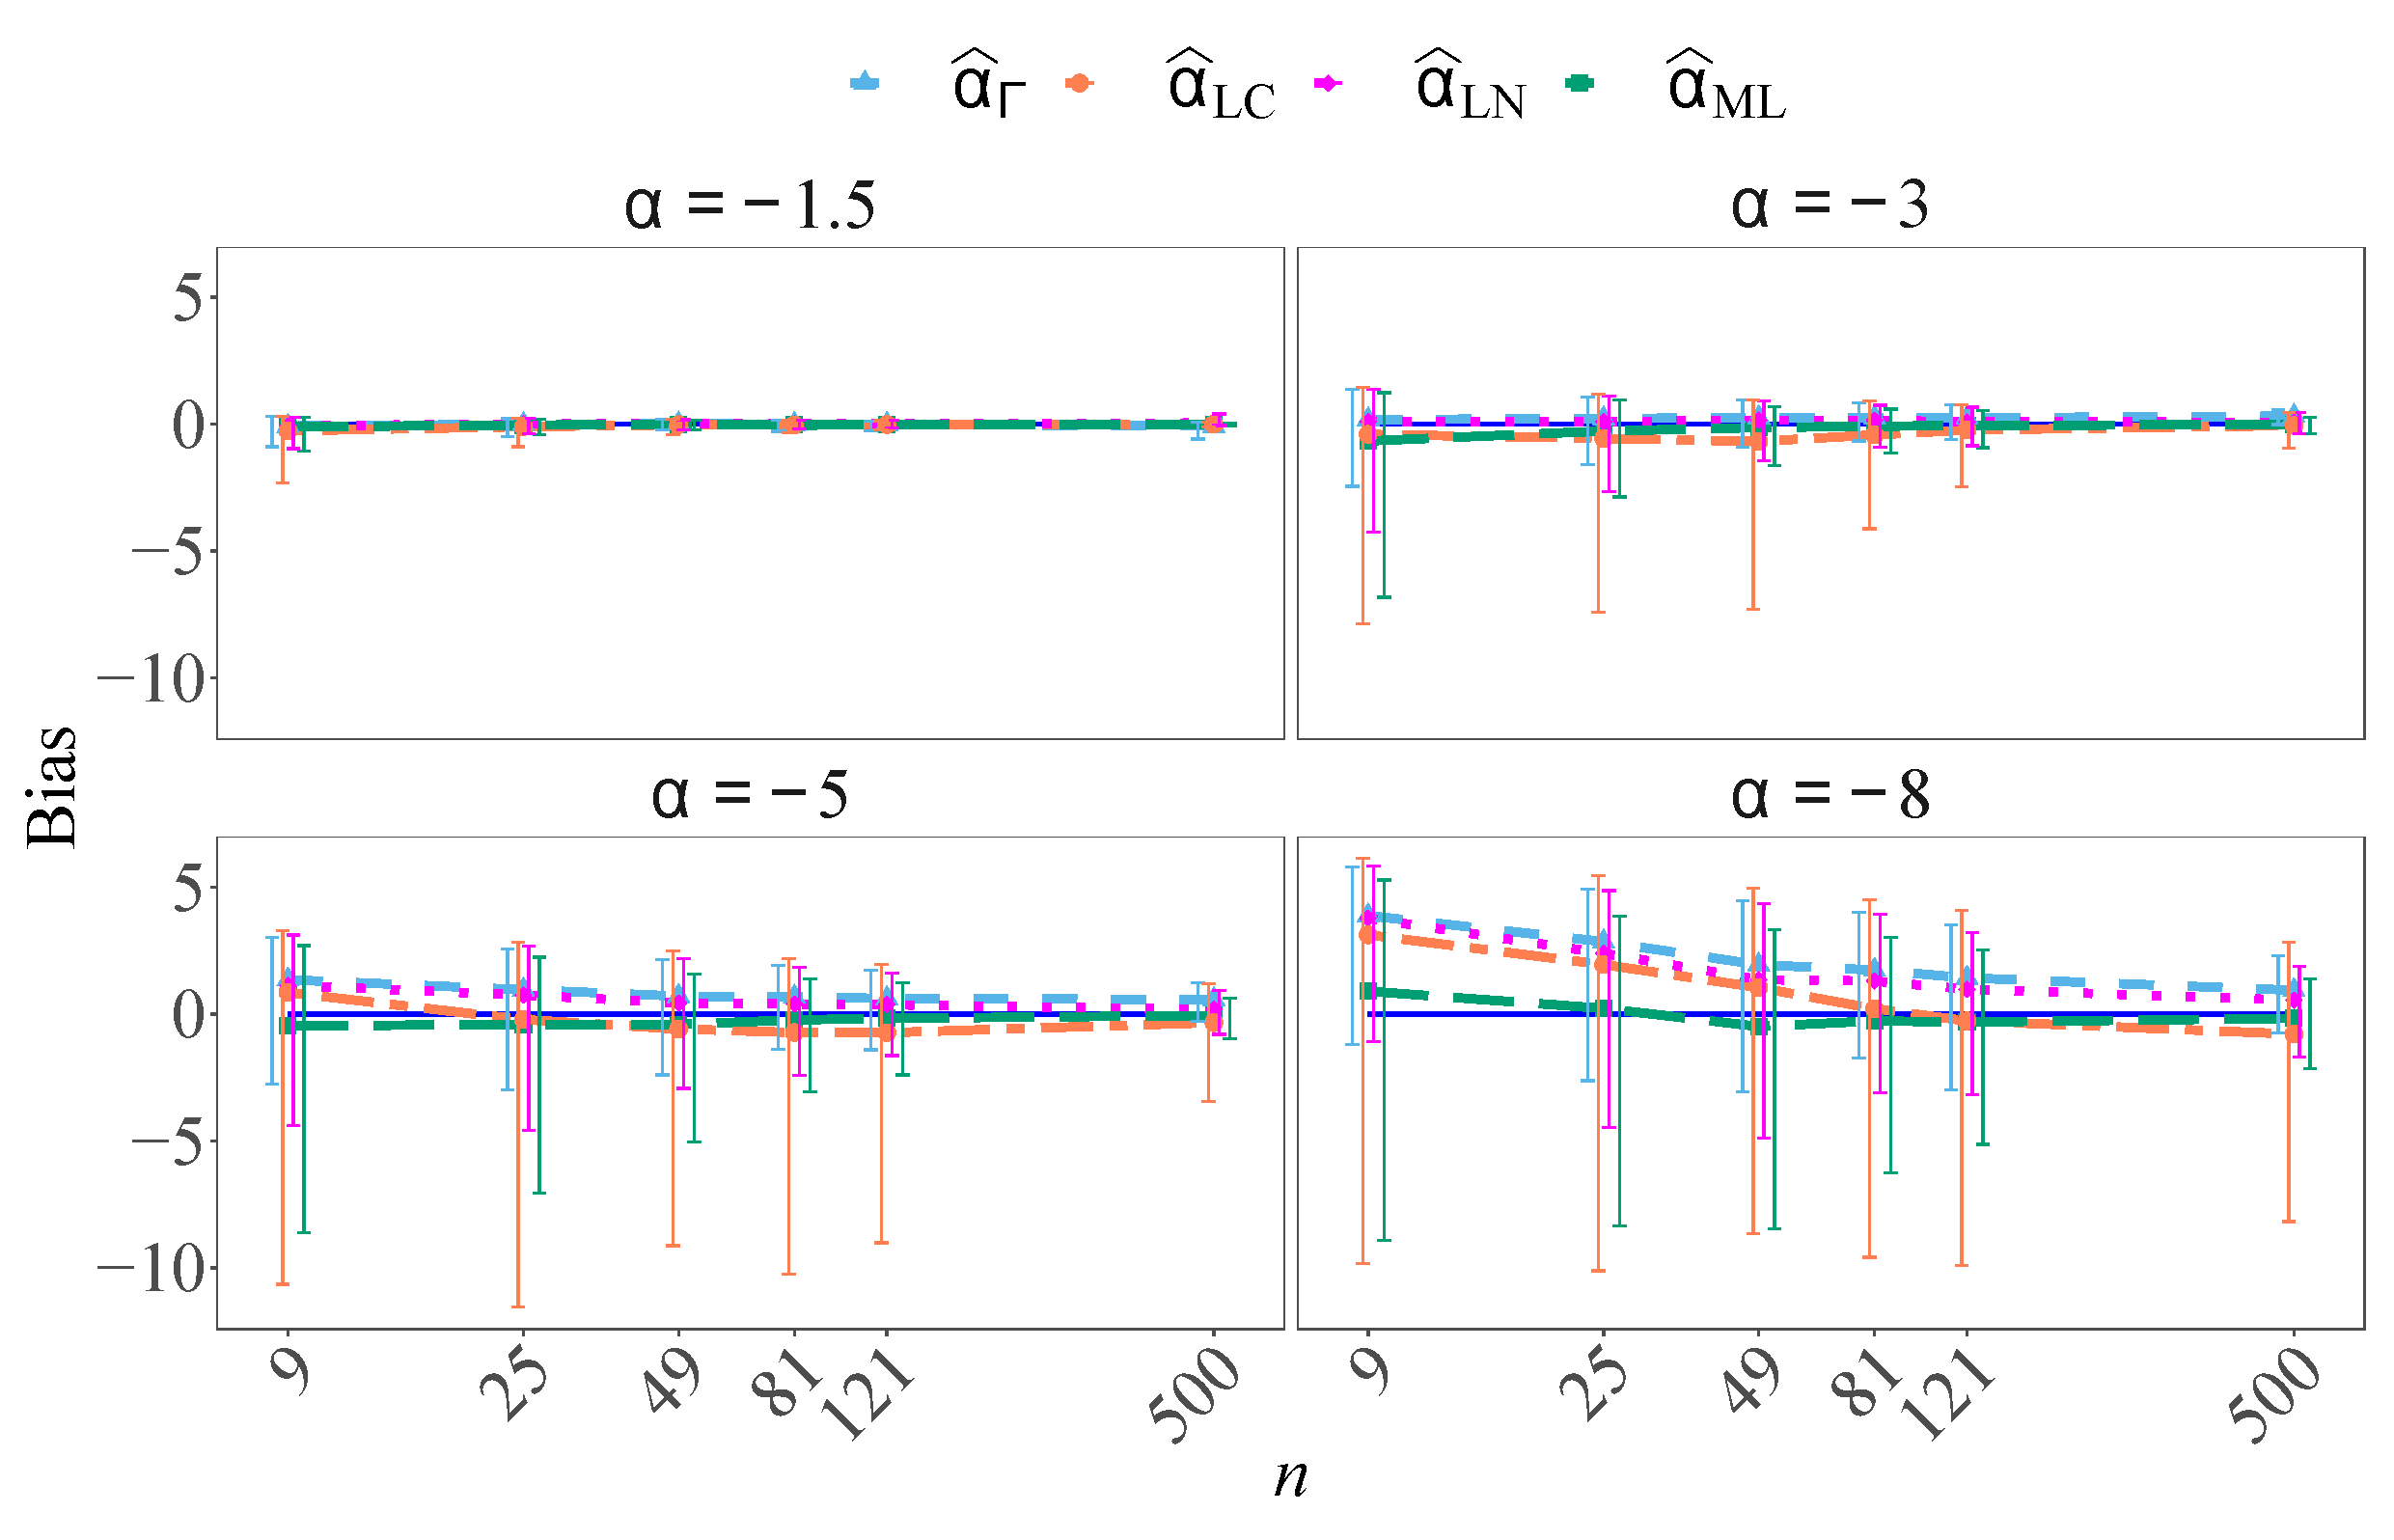
\includegraphics[width=0.9\linewidth]{../../../Figures/PaperTesis/GraficoSesgoMVyGAyLNyLC_L=8SinCont_BarrasErroryPercentil.eps}}
	\subfigure[\label{ECMSinContL=8}$\widehat{\text{MSE}}$]{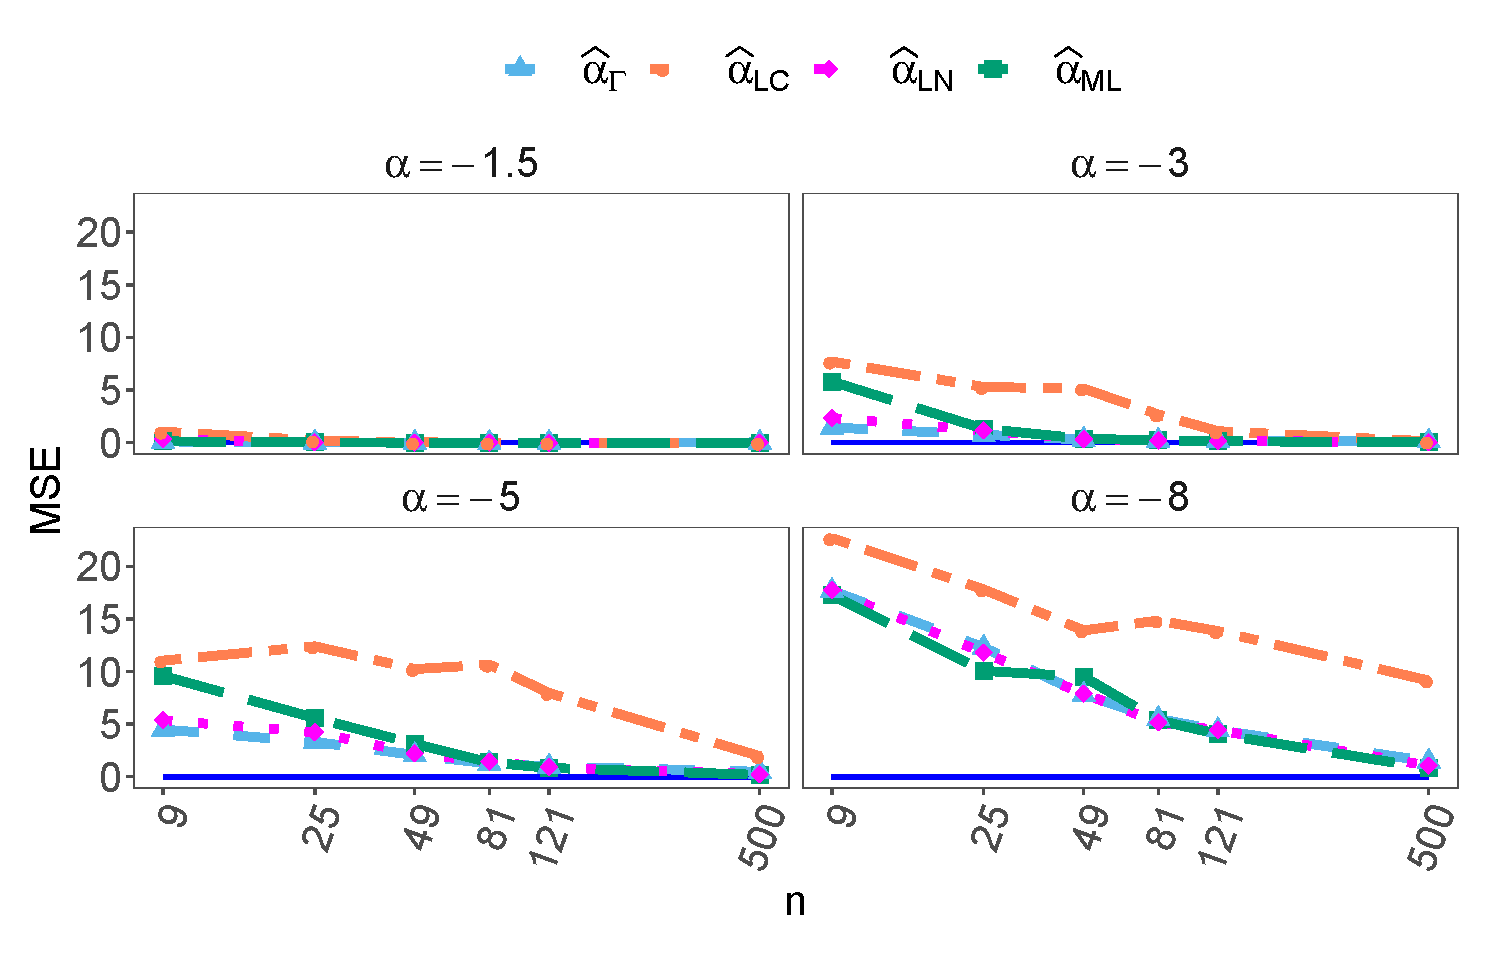
\includegraphics[width=0.9\linewidth]{../../../Figures/PaperTesis/GraficoECMMVyGAyLNyLC_L=8SinCont_BarrasErroryPercentil.eps}}
	\caption{\label{SesgoyECMSinContL=8}\small Bias and MSE estimates for uncontaminated data and $L=8$.}
\end{figure}

According to the study for data without contamination, we conclude that $\widehat{\alpha}_{\text{{LN}}}$ is competitive against the other estimators for uncontaminated data, and that it has better performance than the rest of the methods in some of the cases evaluated.

\subsection{Simulation Results -- Stylized Samples}
\label{StylizedSamples}

Figures~\ref{SEIFL3a} and~\ref{SEIFL3b} show the SEIFs for $L=3$, $n=25$ and, $\alpha=-1.5,-3$ and $\alpha=-5,-8$ respectively. 
The red ticks marks are the maximum and minimum theoretical quantiles, i.e., $F^{-1}_{\alpha,\gamma^*,L}\big(2/(3n+1)\big)$ and $F^{-1}_{\alpha,\gamma^*,L}\big((3n-4)/(3n+1)\big)$, respectively.
The horizontal line is the true value.

\begin{figure}[htb]
	\centering
	\subfigure[\label{InflL3alfa-1.5n25}$\widehat{\alpha}=-1.5$]{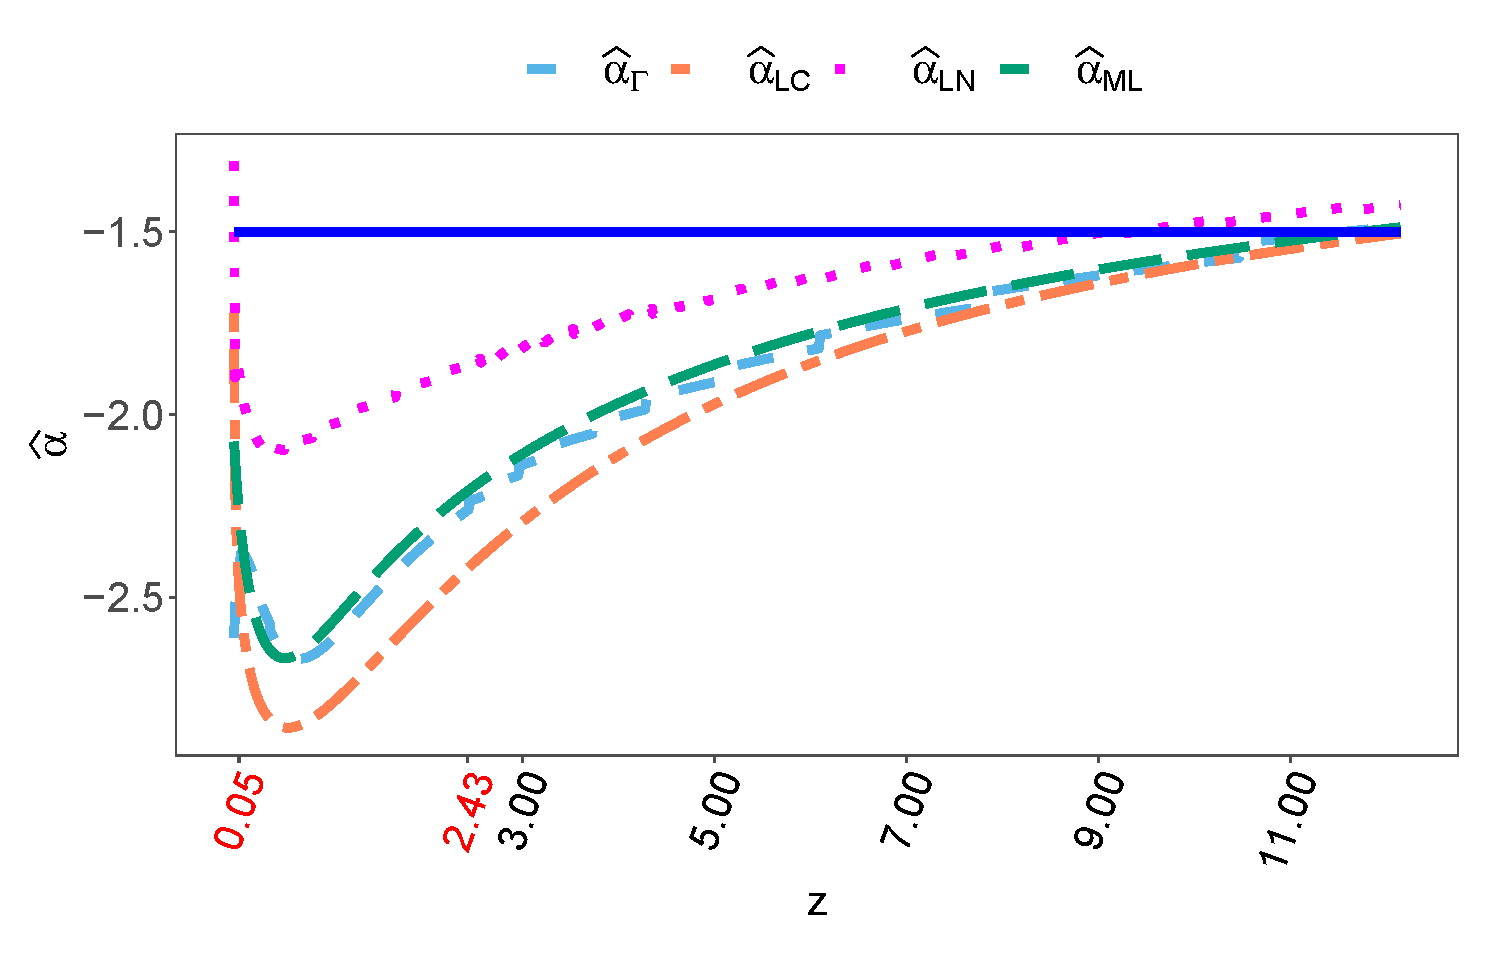
\includegraphics[width=.48\linewidth]{../../../Figures/PaperTesis/CurvaInfluenciaAlfa-1punto5L3n25.eps}}
	\subfigure[\label{InflL3alfa-3n25}$\widehat{\alpha}=-3$]{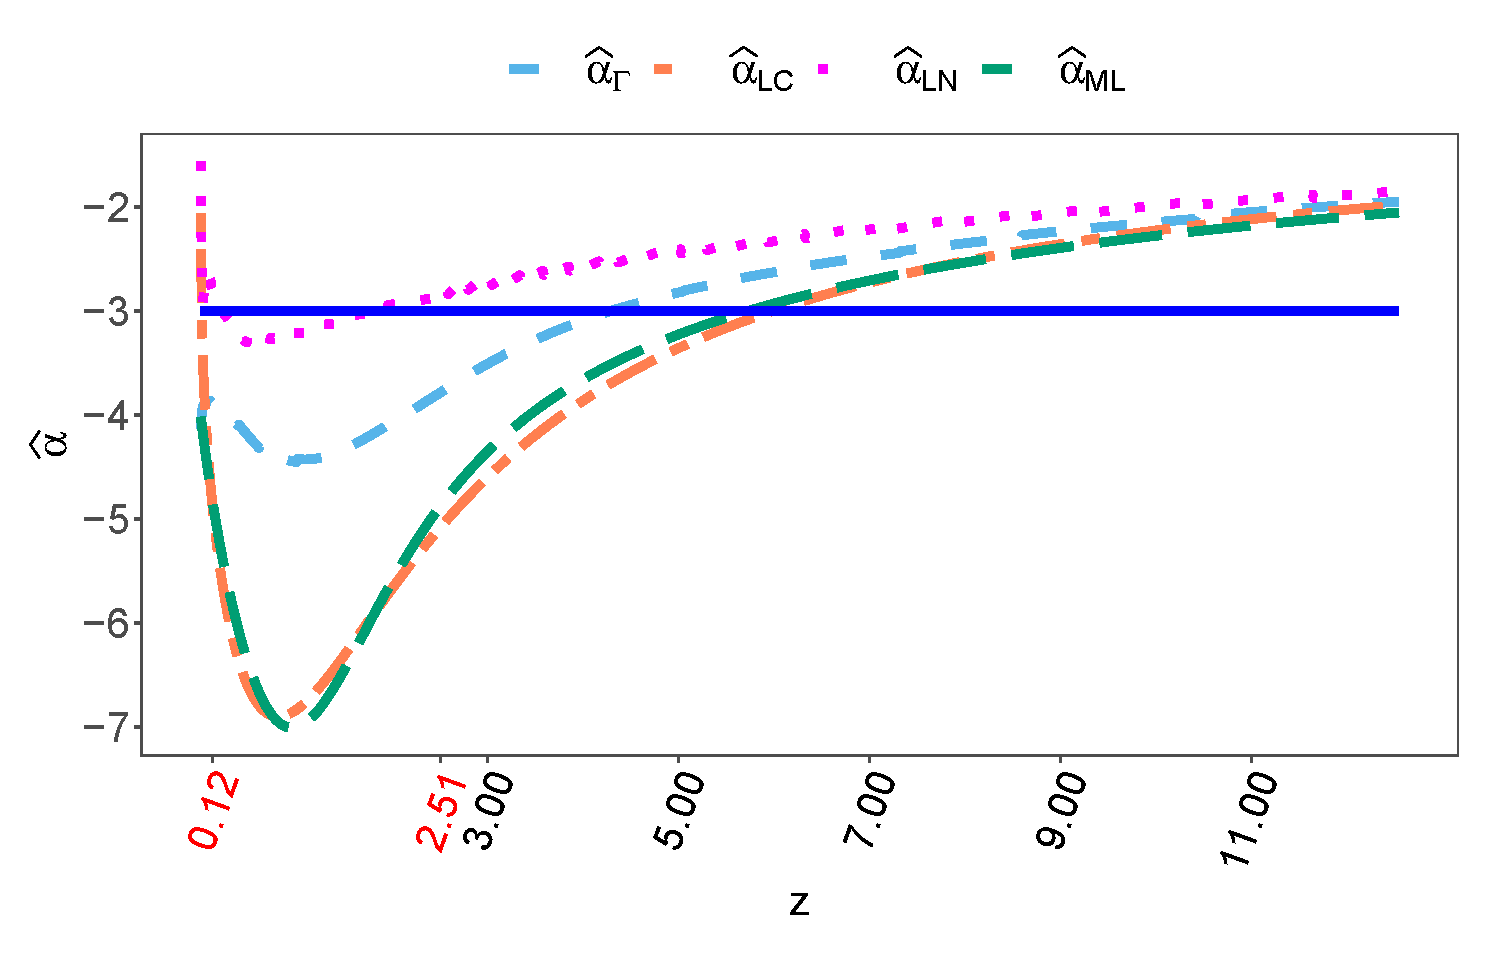
\includegraphics[width=.48\linewidth]{../../../Figures/PaperTesis/CurvaInfluenciaAlfa-3L3n25.eps}}
	\caption{\label{SEIFL3a}\small SEIF for $\widehat{\alpha}_{\text{{ML}}}$, $\widehat{\alpha}_{\Gamma}$, $\widehat{\alpha}_{\text{{LN}}}$, $\widehat{\alpha}_{\text{\tiny{{LC}}}}$ para $L=3$, $n=25$ y $\alpha=-1.5,-3$.}
\end{figure}

\begin{figure}[htb]
	\centering
	\subfigure[\label{InflL3alfa-5n25}$\widehat{\alpha}=-5$]{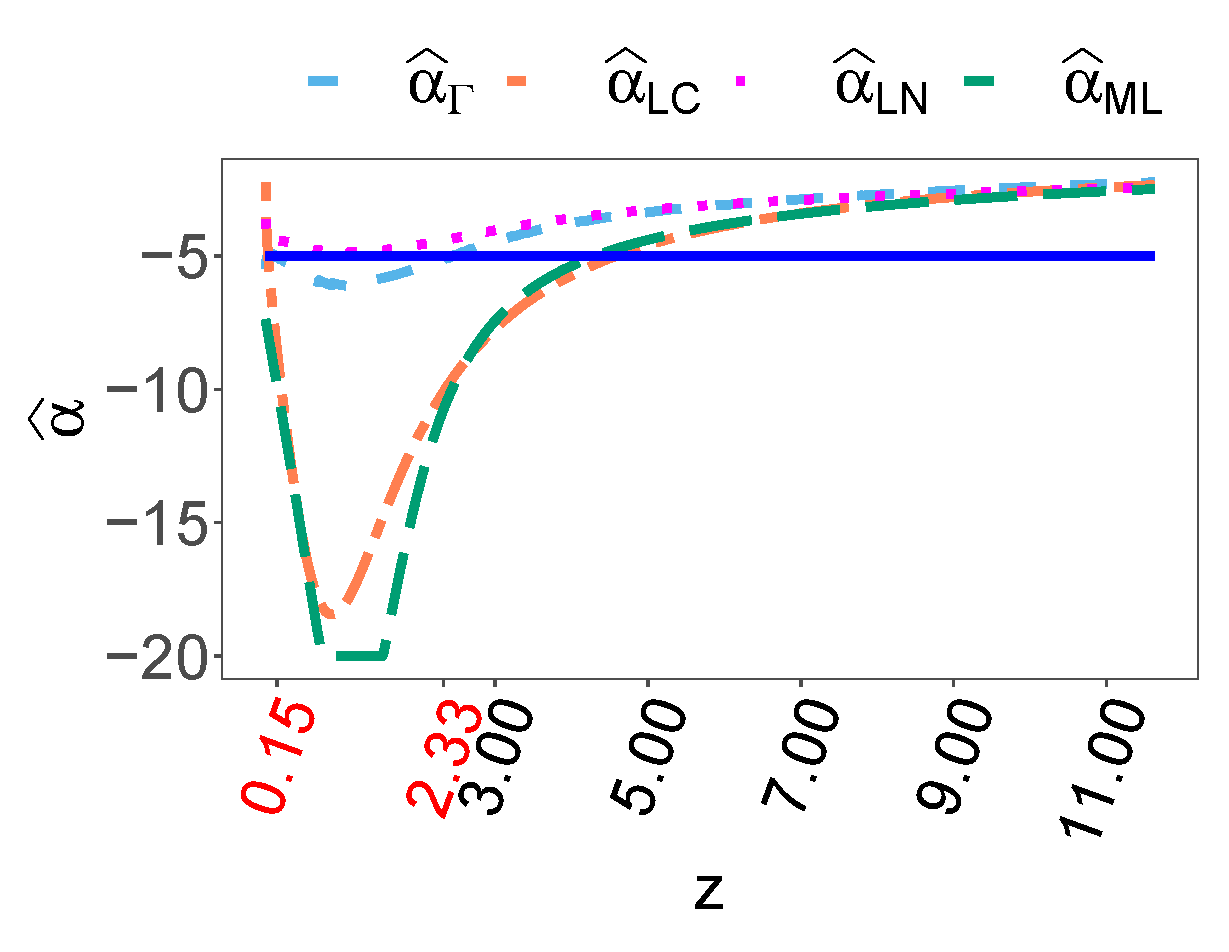
\includegraphics[width=.48\linewidth]{../../../Figures/PaperTesis/CurvaInfluenciaAlfa-5L3n25.eps}}
	\subfigure[\label{InflL3alfa-8n25}$\widehat{\alpha}=-8$]{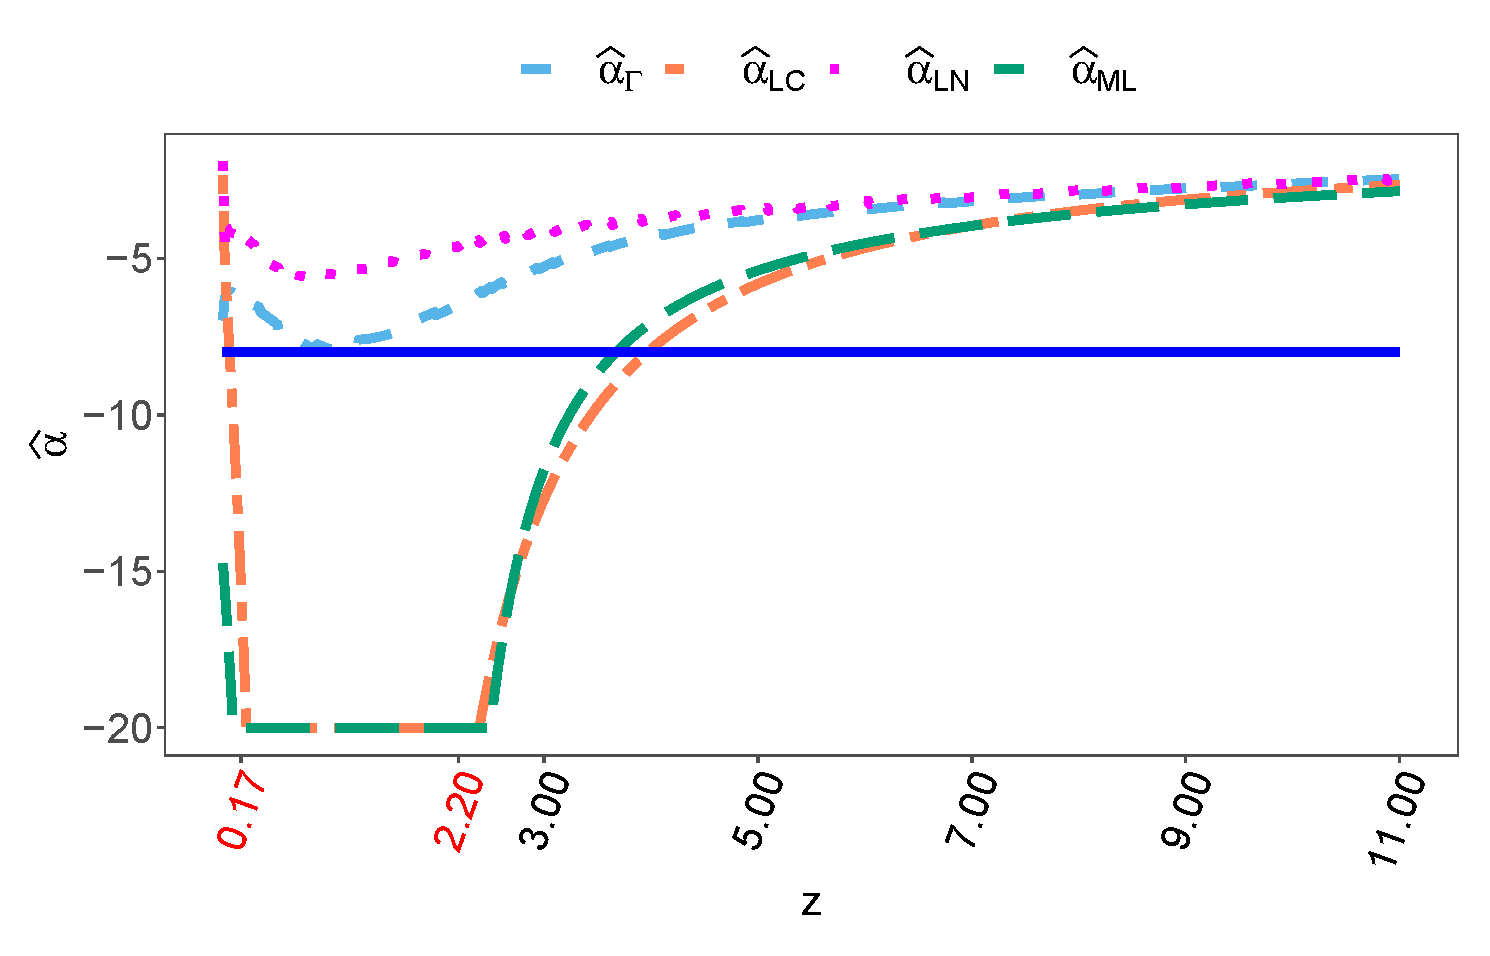
\includegraphics[width=.48\linewidth]{../../../Figures/PaperTesis/CurvaInfluenciaAlfa-8L3n25.eps}}
	\caption{\label{SEIFL3b}\small SEIF for $\widehat{\alpha}_{\text{{ML}}}$, $\widehat{\alpha}_{\Gamma}$, $\widehat{\alpha}_{\text{{LN}}}$, $\widehat{\alpha}_{\text{\tiny{{LC}}}}$ para $L=3$, $n=25$ y $\alpha=-5,-8$.}
\end{figure}

\begin{figure}[htb]
	\centering
	\subfigure[\label{InflL8alfa-1.5n25}$\widehat{\alpha}=-1.5$]{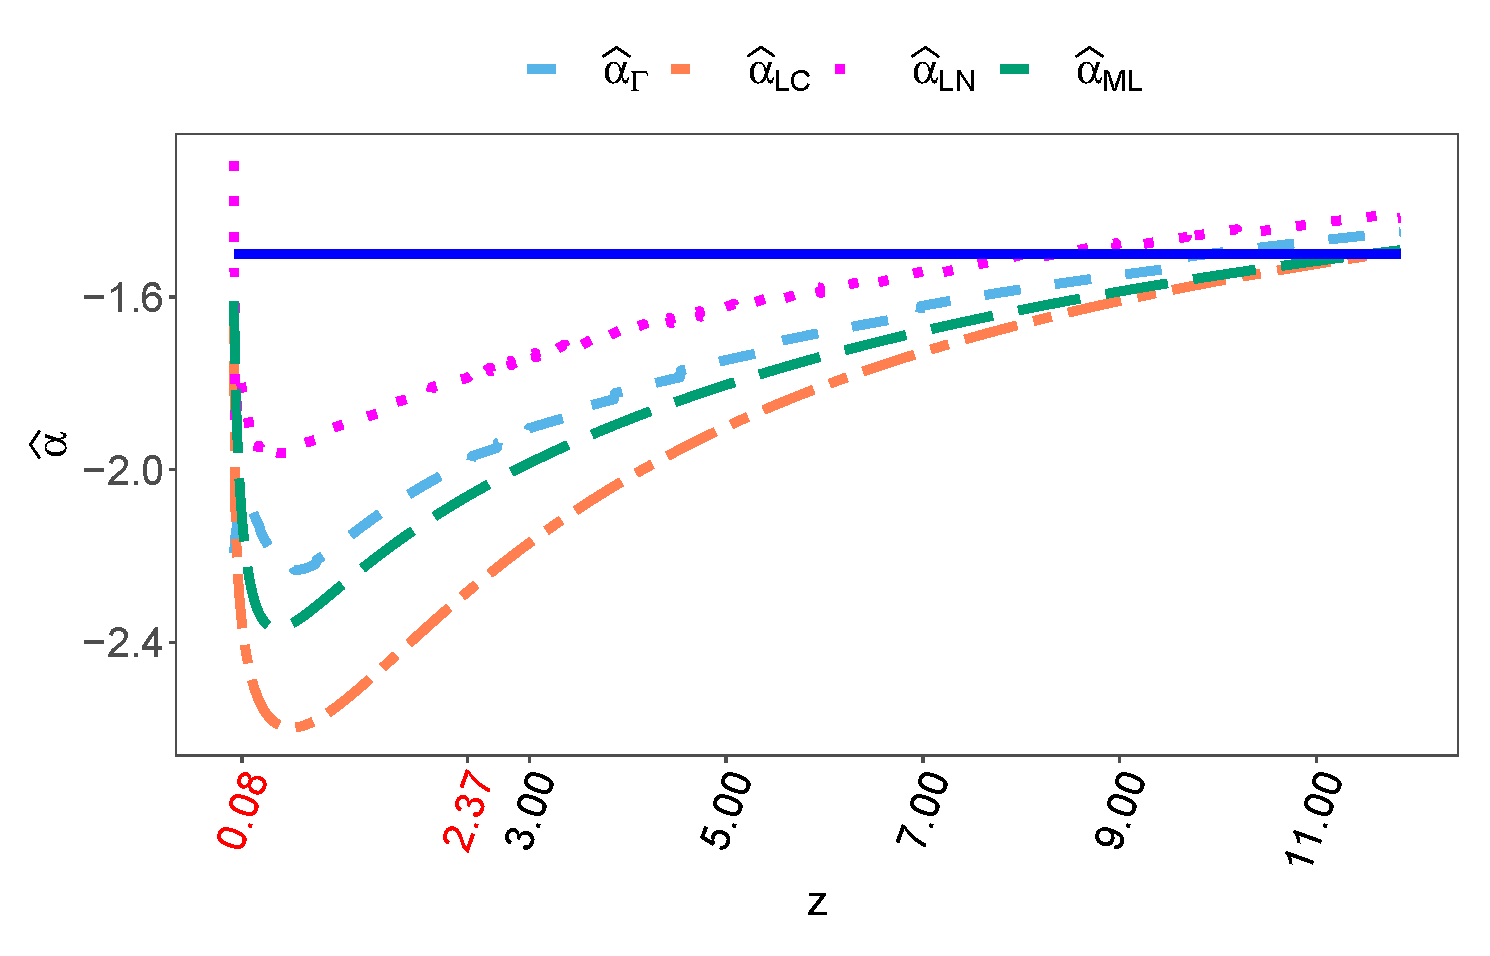
\includegraphics[width=.48\linewidth]{../../../Figures/PaperTesis/CurvaInfluenciaAlfa-1punto5L8n25.eps}}
	\subfigure[\label{InflL8alfa-3n25}$\widehat{\alpha}=-3$]{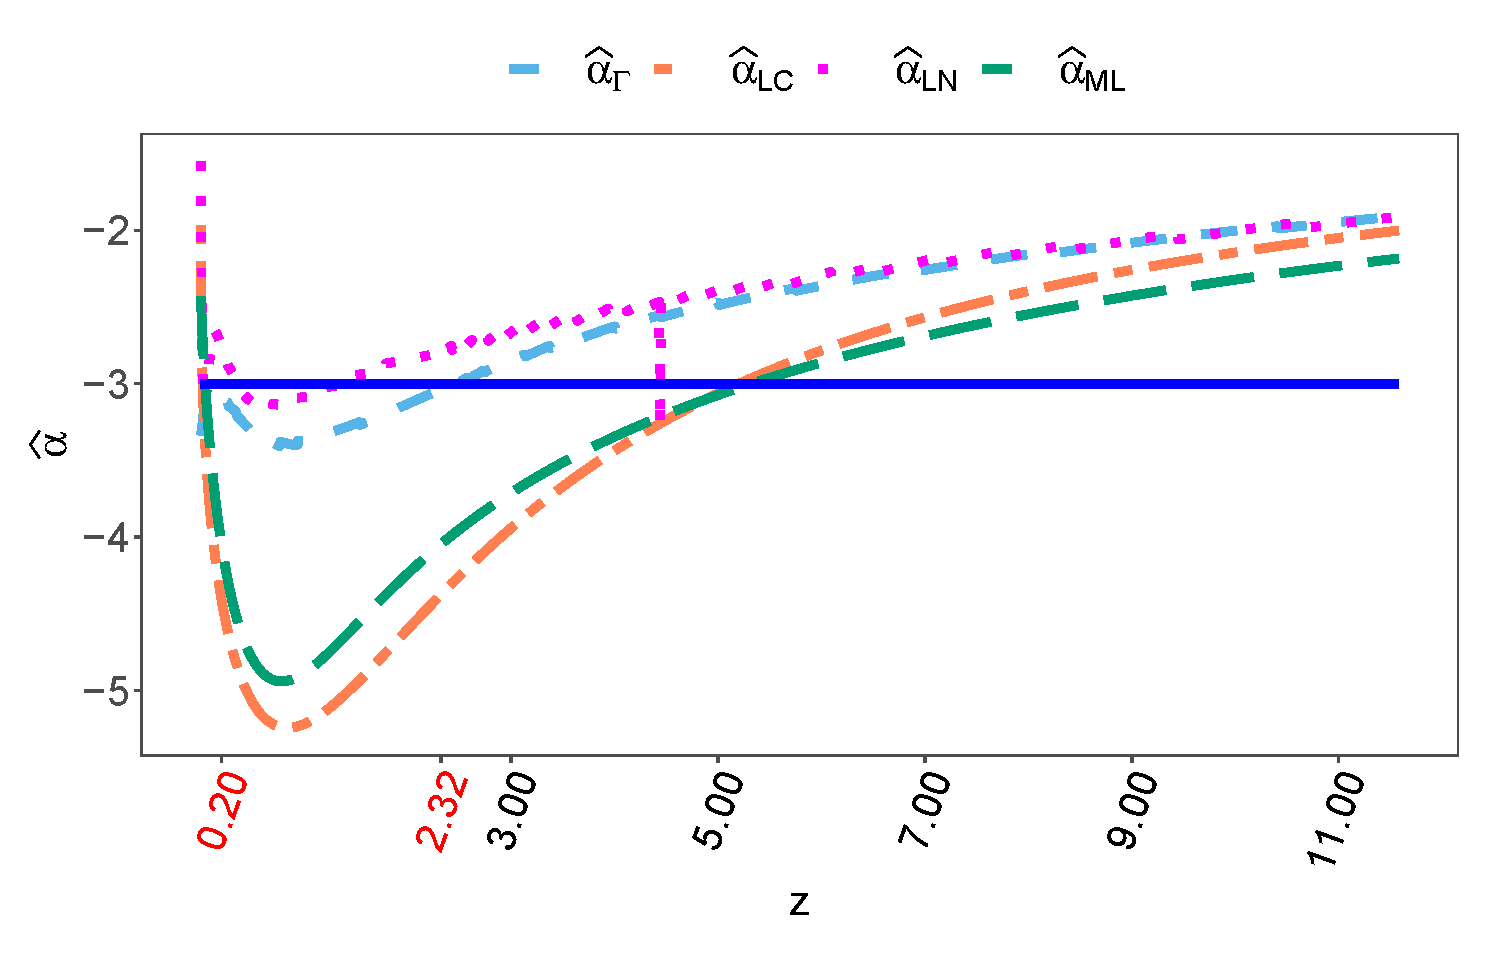
\includegraphics[width=.48\linewidth]{../../../Figures/PaperTesis/CurvaInfluenciaAlfa-3L8n25.eps}}
	\caption{\label{SEIFL8a}\small SEIF for $\widehat{\alpha}_{\text{{ML}}}$, $\widehat{\alpha}_{\Gamma}$, $\widehat{\alpha}_{\text{{LN}}}$, $\widehat{\alpha}_{\text{\tiny{{LC}}}}$ para $L=8$, $n=25$ y $\alpha=-1.5,-3$.}
\end{figure}

\begin{figure}[htb]
	\centering
	\subfigure[\label{InflL8alfa-5n25}$\widehat{\alpha}=-5$]{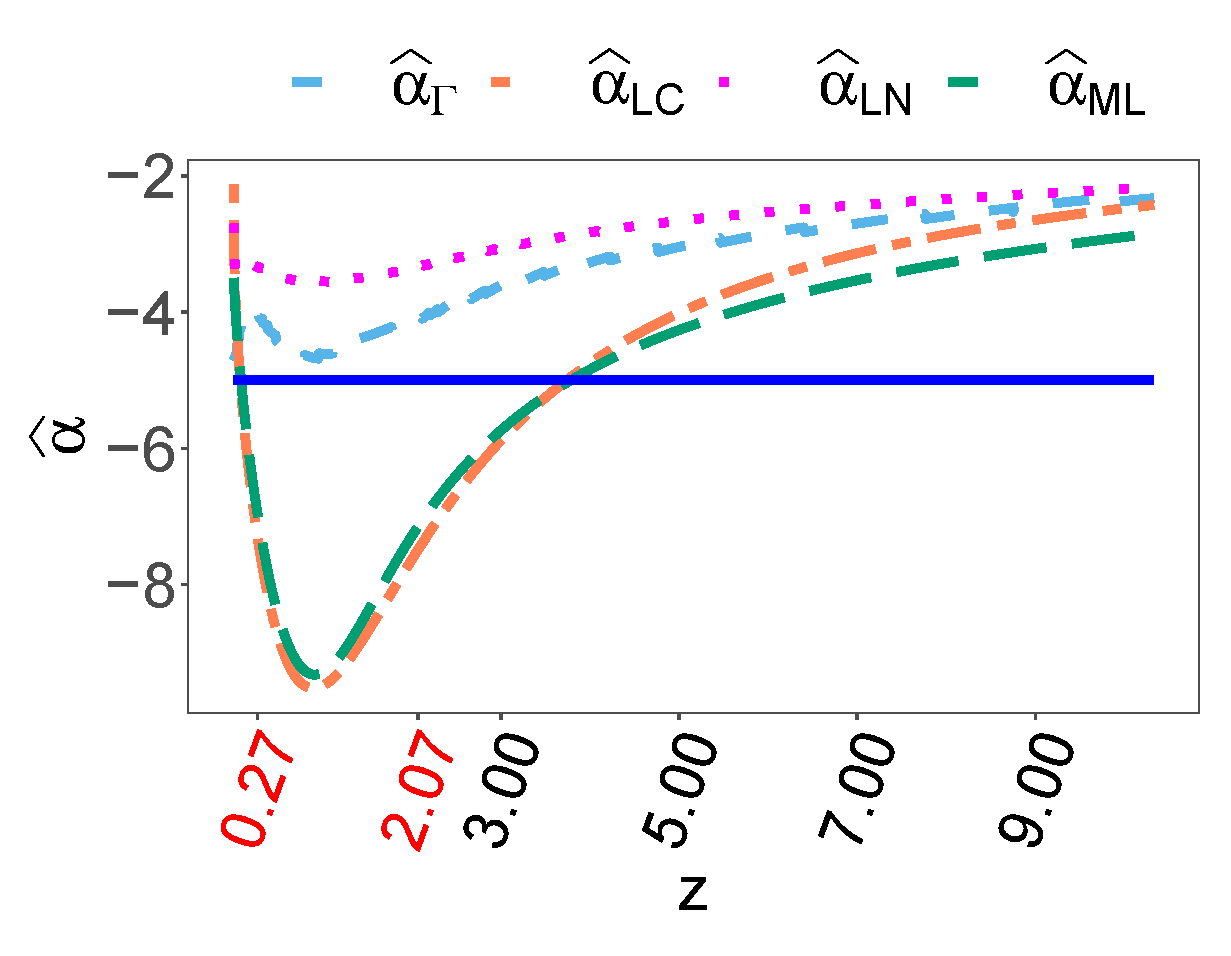
\includegraphics[width=.48\linewidth]{../../../Figures/PaperTesis/CurvaInfluenciaAlfa-5L8n25.eps}}
	\subfigure[\label{InflL8alfa-8n25}$\widehat{\alpha}=-8$]{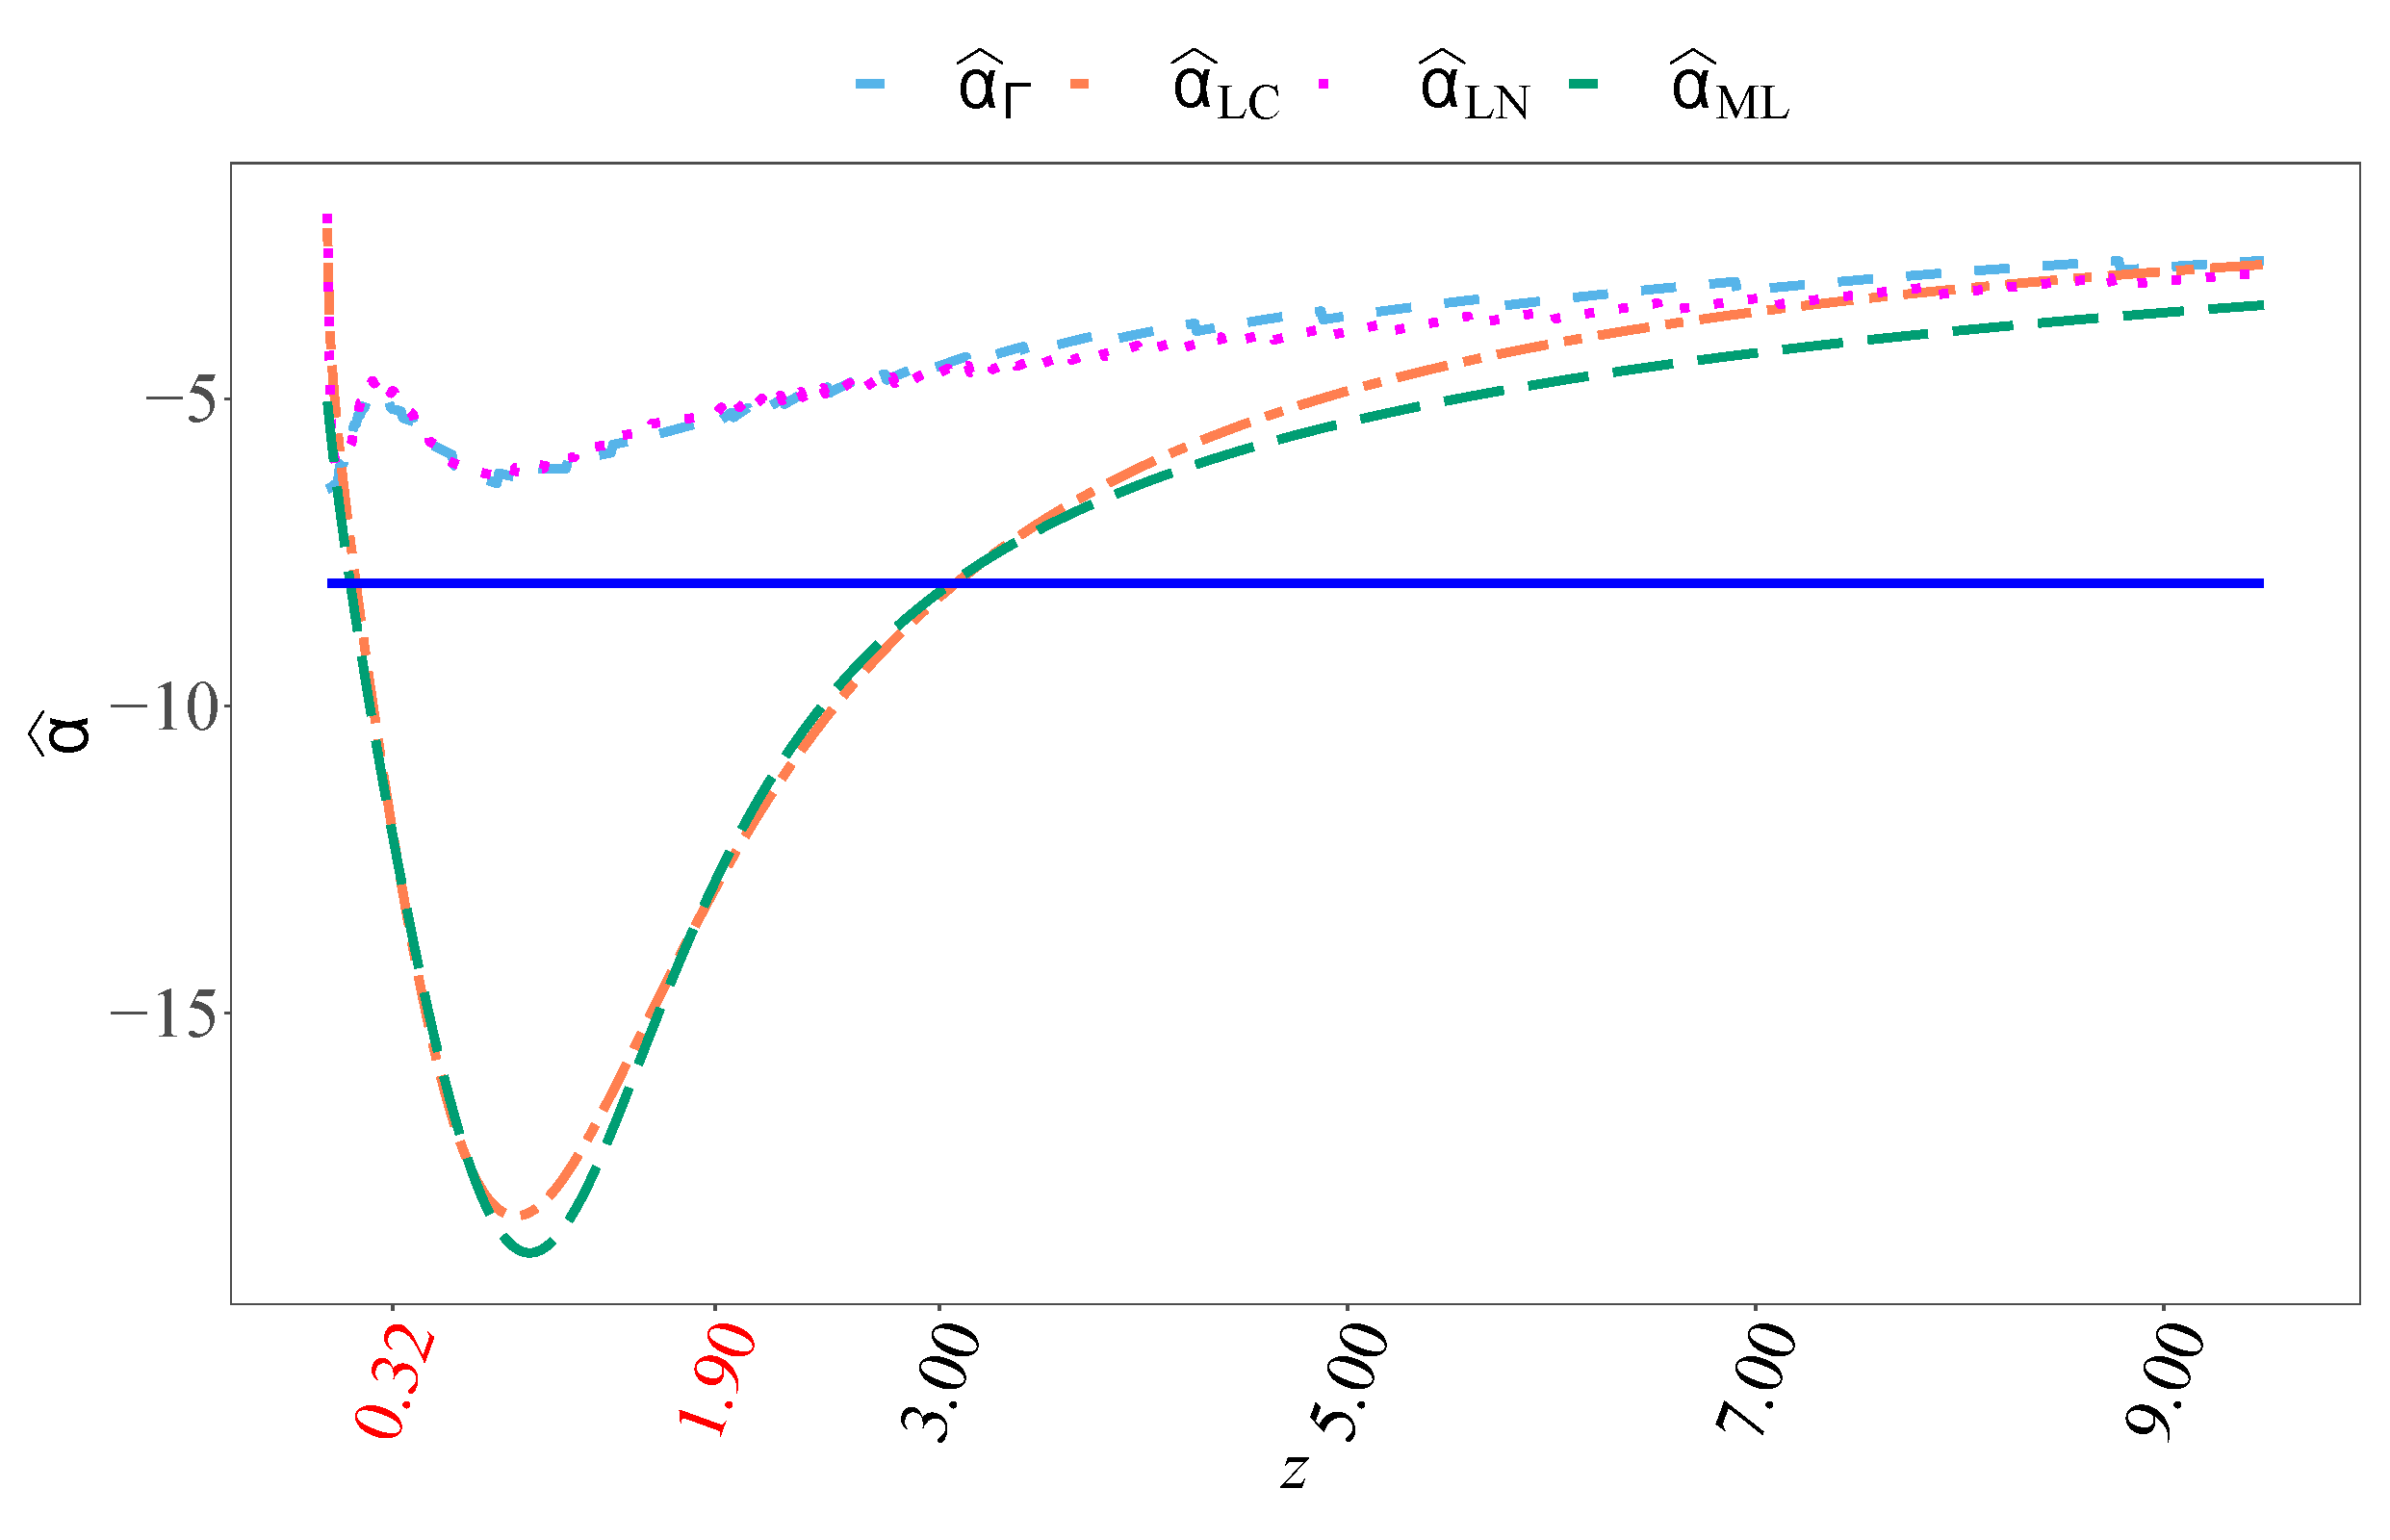
\includegraphics[width=.48\linewidth]{../../../Figures/PaperTesis/CurvaInfluenciaAlfa-8L8n25.eps}}
	\caption{\label{SEIFL8b}\small SEIF for $\widehat{\alpha}_{\text{{ML}}}$, $\widehat{\alpha}_{\Gamma}$, $\widehat{\alpha}_{\text{{LN}}}$, $\widehat{\alpha}_{\text{{LC}}}$ para $L=8$, $n=25$ y $\alpha=-5,-8$.}
\end{figure}

Again a similar behavior can be seen between $\widehat{\alpha}_{\text{{ML}}}$, $\widehat{\alpha}_{\text{{LC}}}$ on the one side, and $\widehat{\alpha}_{\Gamma}$ and $\widehat{\alpha}_{\text{{LN}}}$ on the other for $\alpha=-3, -5, -8$. 
In extremely textured areas $\widehat{\alpha}_{\text{{LN}}}$ has the best performance, while for $z$ values lower than the last quantile and for the rest of the textures, both $\widehat{\alpha}_{\Gamma}$ and $\widehat{\alpha}_{\text{{LN}}}$ have a better performance compared to the other estimators. 
Moreover, $\widehat{\alpha}_{\text{{ML}}}$ does not converge for moderately heterogeneous and homogeneous zones, while $\widehat{\alpha}_{\text{{LC}}}$ does not converge for homogeneous zones. All estimators behave similarly for large values of $z$. 
This behavior shows the sensitivity and loss of robustness for $\widehat{\alpha}_{\text{{ML}}}$ and $\widehat{\alpha}_{\text{{LC}}}$ versus MDEs.

Figures~\ref{InflL8alfa-1.5n25}, \ref{InflL8alfa-3n25}, \ref{InflL8alfa-5n25} and~\ref{InflL8alfa-8n25} show the SEIFS for $L=8$ and the same values of $n$ and $\alpha$. 
The performance of the estimators for this case is similar to that described for $L=3$. 
It should be mentioned that all methods converge for this case where there is less presence of speckle noise.

%%%%%%%%%%%%%%%%%%%%%%%%%%%%%%%%%¨

\subsection{Simulation Results -- Contamination Data}
\label{CasesCont}

%A property that is desirable for an estimator is to be resistant to the presence of outliers. 
%
%It is very important to have estimators that are resistant to the presence of contaminated data, that is, that are capable of producing good estimation even when a proportion of the data does not come from the assumed model. This situation is of particular importance when filters are used because they range the image through sliding windows of size $3\times 3$, $5 \times 5$ or, for example, $7 \times 7 $. These samples may have data from areas with different degrees of texture, for example, at the border between different regions. 
%
%Bustos et al.~\cite{BustosFreryLucini:Mestimators:2001} and Allende et al.~\cite{AllendeFreryetal:JSCS:05} studied the performance of the ML estimator under the $\mathcal{G}^{0}$ model for amplitude data, showing that there is a loss of robustness in the presence of moderate outliers in extremely textured areas, while for textured areas these lost occurs in the presence of severe outliers. This lack of robustness is also more pronounced in the case of small samples. They proposed as an alternative the M and AM estimators that have good behavior under contamination but present numerical problems especially for small sample sizes.
%
%One of contamination sources in SAR images is the Double Bounce phenomenon, where some pixels have a high return value. The presence of such outliers can cause large errors in the estimate. The description of this phenomenon can be seen in~\cite{DobleBounce}.
%
%We propose two ways to evaluate the robustness of the estimators, one is generate contaminated samples where $0 <\epsilon \ll 1$ is the proportion of contamination. The other is studying the SEIF.
%
%Let $B$ be a Bernoulli random variable with a $p$ probability of contamination occurrence. Let $W$   and $U$ be such that $W \sim \mathcal{G}^0(\alpha_1,\gamma_1^*,L)$,  and $U \sim \mathcal{G}^0(\alpha_2,\gamma_2^*,L) $. Define $Z=BU+(1-B)W$, then we generate $\{z_1,\dots,z_n\}$ identically distributed random variables with cumulative distribution function 
%$$
%(1-\epsilon) \mathcal{F}_{\mathcal{G}^0(\alpha_1,\gamma_1^*,L)}(z)+\epsilon\mathcal{F}_{\mathcal{G}^0(\alpha_2,\gamma_2^*,L)}(z),
%$$
%where $\mathcal{F}_{\mathcal{G}^0(\alpha,\gamma,L)}$ is the cumulative distribution function of a $\mathcal{G}^0(\alpha,\gamma,L)$ random variable.
%
In the following, we show the performance, throughout the bias and mean square error, of the estimators under contamination. 
Figures~\ref{SesgoyECMConContL=3} and~\ref{SesgoyECMConContL=8} present these quantities under contaminated data for $L=3$ and $L=8$ respectively. In this case we considered $\epsilon=0.05$

%%%%%%%%%%%%%%%%%% EPSILON 0.05
\begin{figure}[htb]
	\centering
	\subfigure[\label{SesgoConContL=3}$\widehat{\text{Bias}}$]{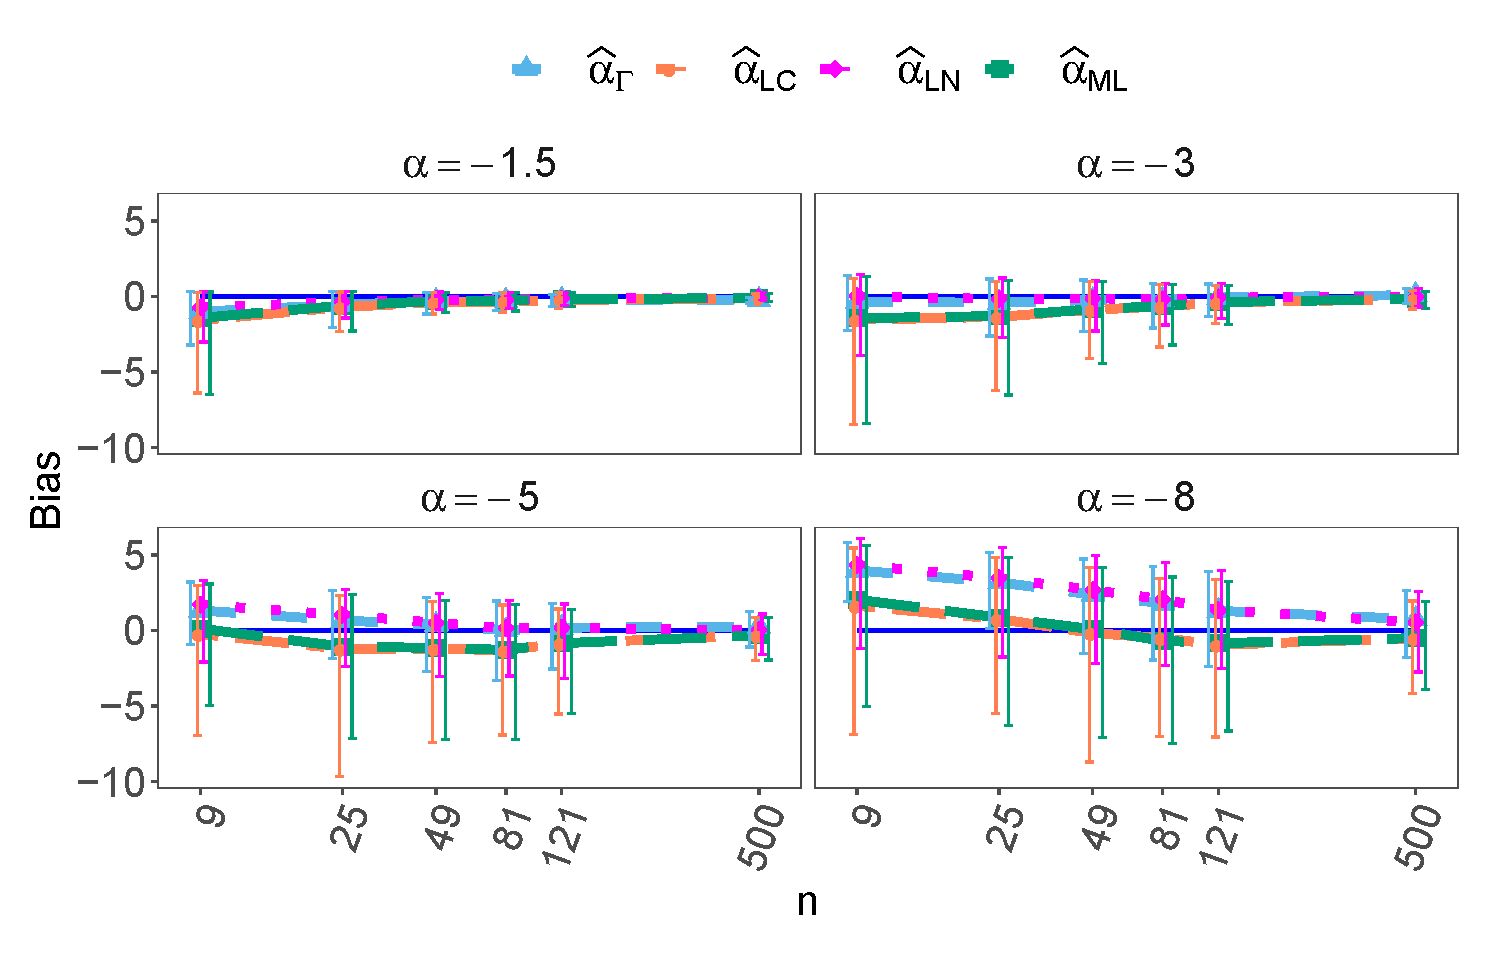
\includegraphics[width=.8\linewidth]{../../../Figures/PaperTesis/GraficoSesgoMVyGAyLNyLC_L=3Cont_BarrasErrorypercentil.eps}}
	\subfigure[\label{ECMConContL=3}$\widehat{\text{MSE}}$]{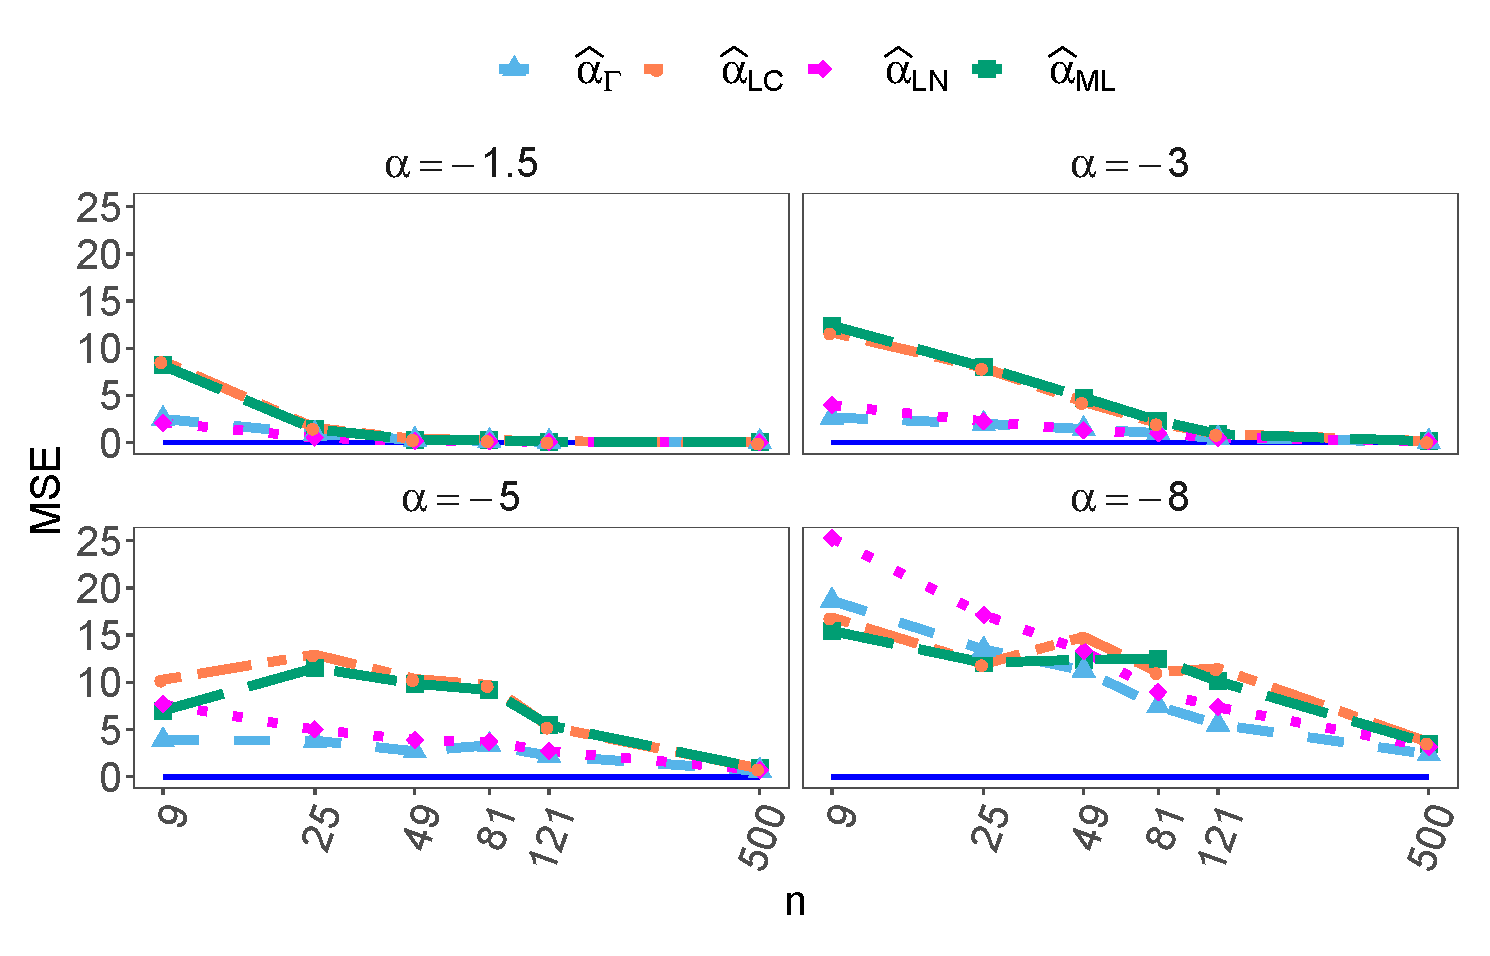
\includegraphics[width=.8\linewidth]{../../../Figures/PaperTesis/GraficoECMMVyGAyLNyLC_L=3Cont_BarrasErrorypercentil.eps}}
	\caption{\label{SesgoyECMConContL=3}\small Bias and MSE for contaminated data,  $\epsilon=0.05$ and $ L=3$.}
\end{figure}

\begin{figure}[htb]
	\centering
	\subfigure[\label{SesgoConContL=8}$\widehat{\text{Bias}}$]{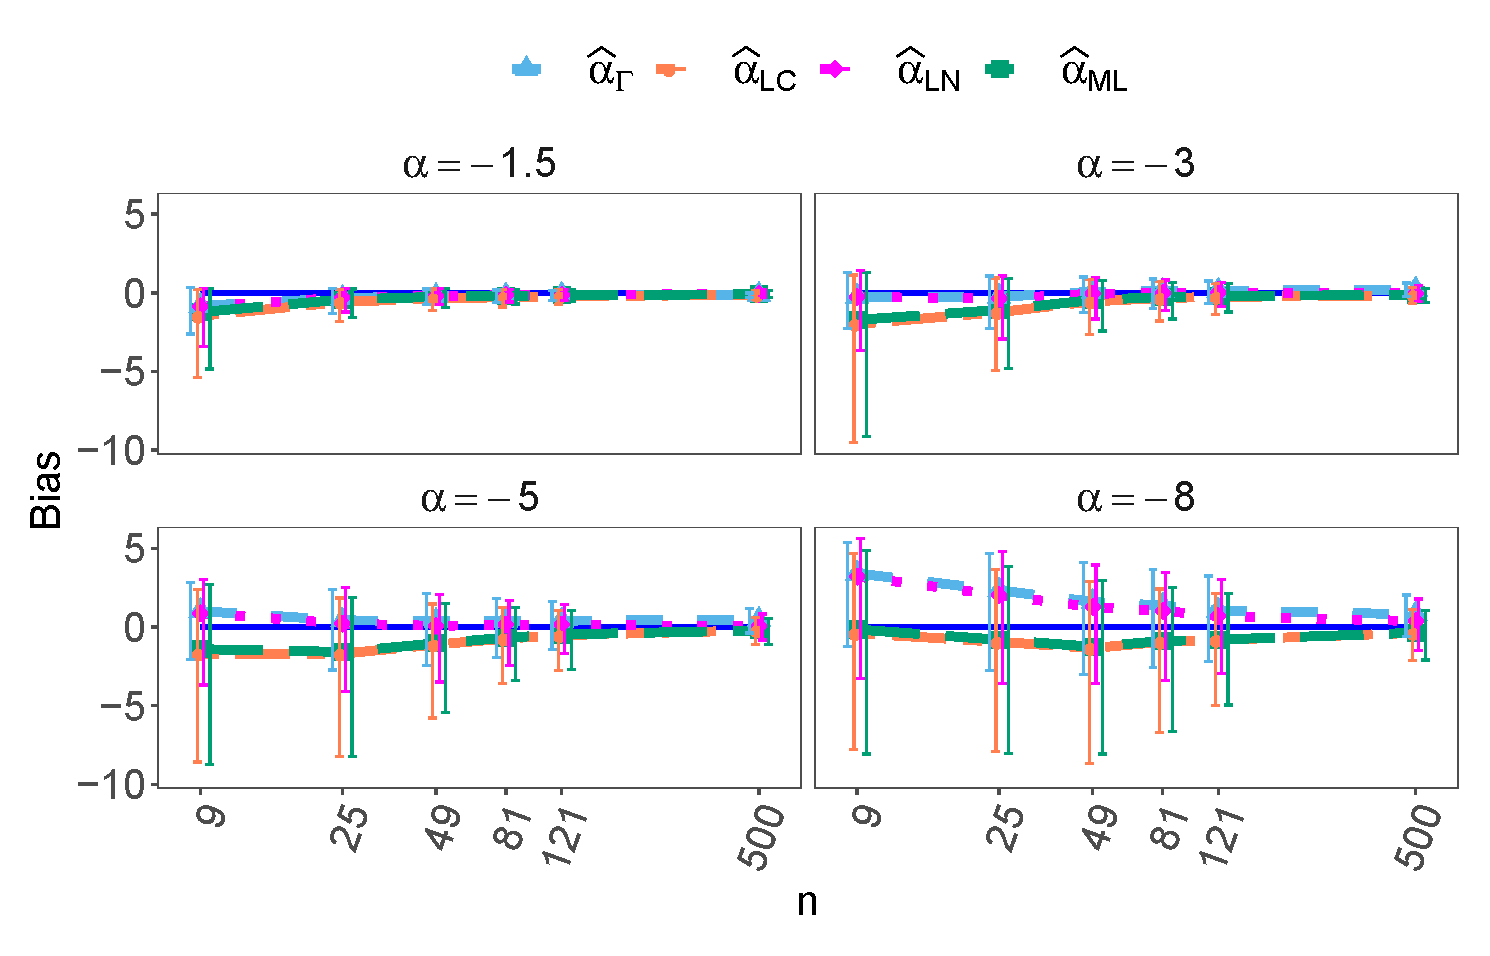
\includegraphics[width=.8\linewidth]{../../../Figures/PaperTesis/GraficoSesgoMVyGAyLNyLC_L=8Cont_BarrasErrorypercentil.eps}}
	\subfigure[\label{ECMConContL=8}$\widehat{\text{MSE}}$]{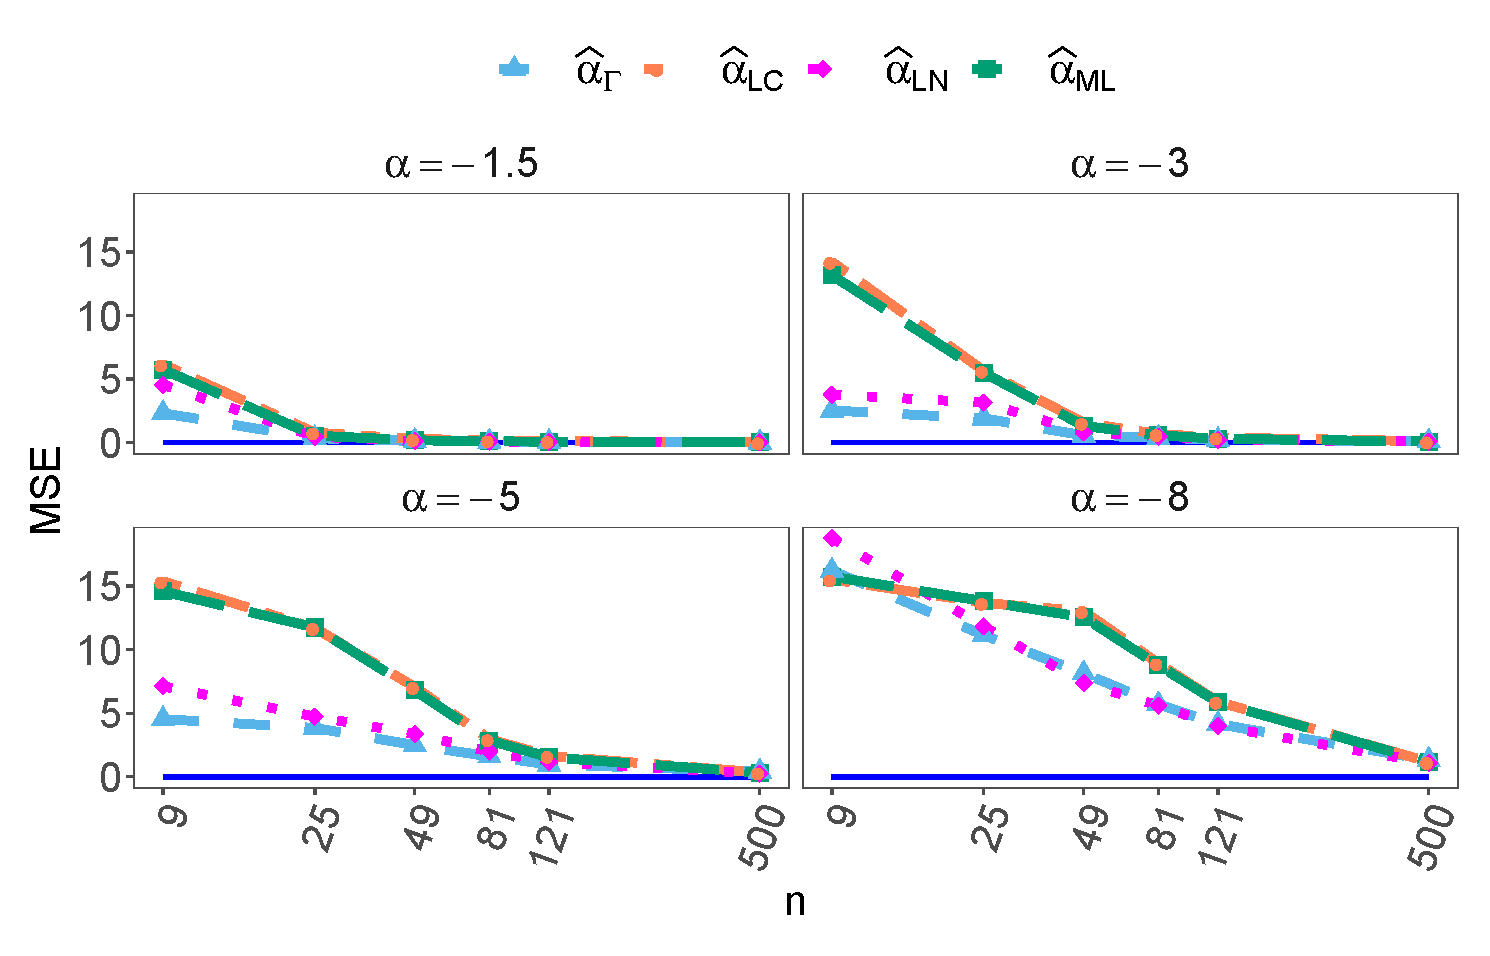
\includegraphics[width=.8\linewidth]{../../../Figures/PaperTesis/GraficoECMMVyGAyLNyLC_L=8Cont_BarrasErrorypercentil.eps}}
	\caption{\label{SesgoyECMConContL=8}\small Bias and MSE for contaminated data,  $\epsilon=0.05$ and $ L=8$.}
\end{figure}


At this level of contamination, it can be seen more clearly how the estimators are grouped by performance, $\widehat{\alpha}_{\text{{ML}}}$ and $\widehat{\alpha}_{\text{{LC}}}$ have suchlike behavior, while the same happens with $\widehat{\alpha}_{\Gamma}$ and $\widehat{\alpha}_{\text{{LN}}}$.  
The difference is noticeable, both in bias and in MSE, in favor of the MDE estimators for large values of $\alpha$. 
In the majority of the cases studied, the MDE estimators have shorter intervals than the other estimators. 
In moderately textured areas, all methods are comparable although the MDE estimators have lower MSE. 
For homogeneous areas $\widehat{\alpha}_{\text{{ML}}}$ and $\widehat{\alpha}_{\text{{LC}}}$ have lower bias although greater variability.

%According to this analysis and to the study of the SEIF, the $\widehat{\alpha}_{\text{{LN}}}$ estimator is the one that presents the best performance for both contaminated and uncontaminated data, for textured areas.

\section{Application to actual data}
\label{application}

We applied the four estimation techniques methods to an actual image from the surroundings of Munich, Germany, obtained by the E-SAR system~\cite{Horn1996} in L~band, HH~polarization, and intensity format. 
This image has $300\times250$ pixels and mainly comprises two different growth areas.

The original image is single-look.
In order to obtain comparable multilook data, we computed new pixels averaging the intensity values in $2\times2$ non-overlapping windows. This technique is known as pyramidal processing~\cite{Adelson1984}, and the resulting image is multilook.

The number of looks, defined by ${\text{E}(I)^2}/{\text{Var}(I)}$ in textureless areas, is not known, but it can be estimated by the equivalent number of looks (ENL) using uncorrelated data and the moment estimator
$\text{ENL}={1}/{\widehat{\text{CV}^2}}$, the reciprocal of the sample coefficient of variation $\widehat{\text{CV}}={\widehat{\sigma}}/{\widehat\mu}$, where $\widehat{\sigma}$ is the sample standard deviation and $\widehat\mu$ the sample mean.
In order to find the $\text{ENL}$ we selected manually four textureless areas and calculated $\text{ENL}_i$ for $i=1, \ldots, 4$. 
The final $\text{ENL}$ is their average weighted by the size of the areas. 
We then set $\widehat L=3.21$ in the analysis of the multilook image.

%	Figure~\ref{MuestraLooks} shows the ESAR multilook image together with the samples used to obtain $\text{ENL}$. 
%	
\begin{figure}[htb]
	\centering
	%\subfigure[\label{MuestraLooks}Samples used to estimate ENL]{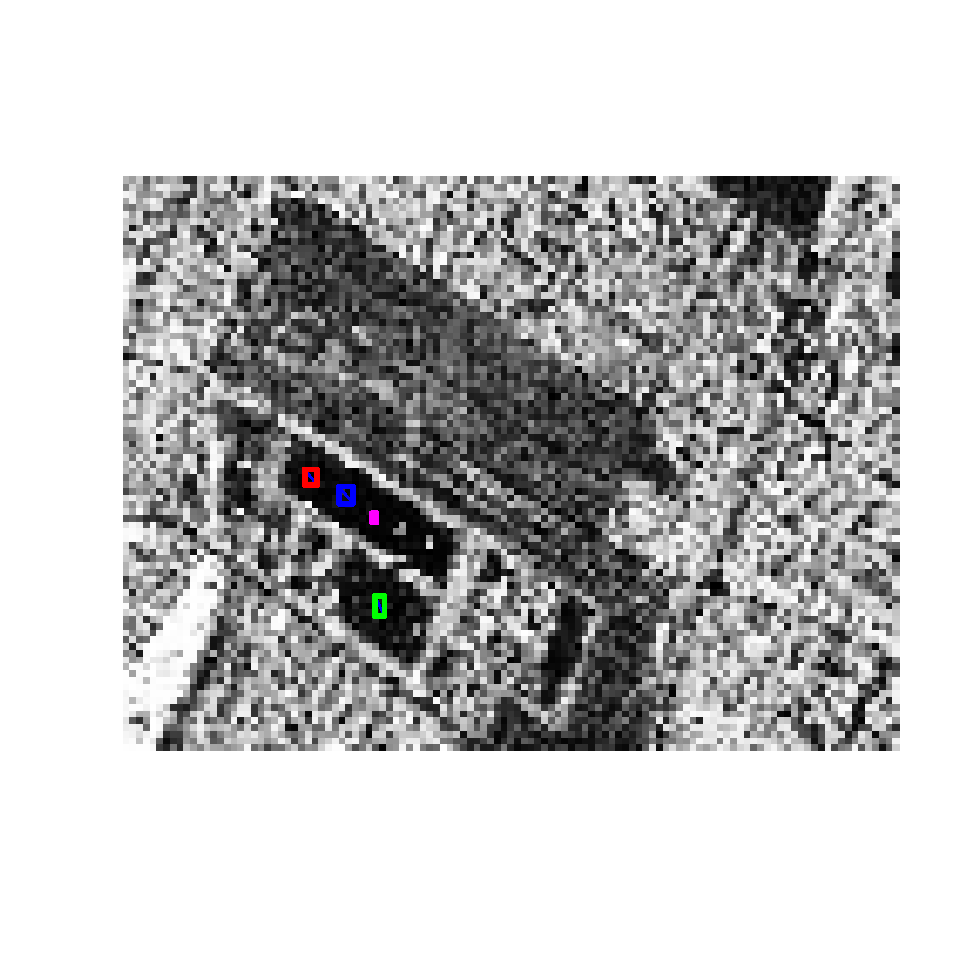
\includegraphics[width=0.48\linewidth]{../../../Figures/PaperTesis/MuestrasEstimNumLooks}}
	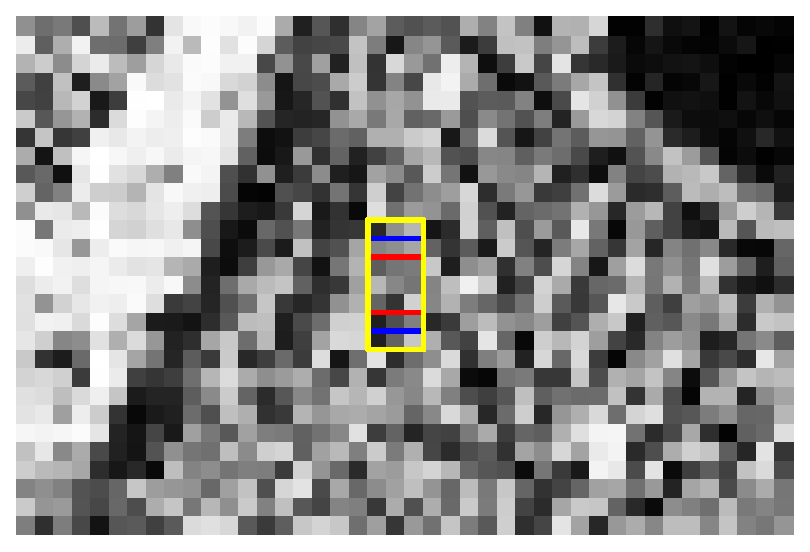
\includegraphics[width=0.8\linewidth]{../../../Figures/PaperTesis/TresMuestrasAgrandada.eps}
	\caption{\label{TresMuestras}\small Samples used to estimate $\widehat{\alpha}$.}
\end{figure}

Figure~\ref{TresMuestras} shows three samples: yellow, red, and blue. 
The size of the first two is $16$, and the latter has size $12$. 
The red sample is a shift from the yellow one in a row of the image data matrix, and the blue sample is contained within the yellow sample.

%%% ACF Always inform the values in the text
Table~\ref{TablaTresMuestras} shows the estimates obtained with the four methods in each sample. 
It can be seen that the estimates differ considerably in the yellow sample: 
both $\widehat{\alpha}_{\text{{ML}}}=-7.21$ and $\widehat{\alpha}_{\text{{LC}}}=-6.74$ are compatible with a homogeneous zone, while $\widehat{\alpha}_{\Gamma}=-4.34$ indicates that it is a heterogeneous one, and $\widehat{\alpha}_{\text{{LN}}}=-3.23$ is on the limit of affirming whether the area is heterogeneous or extremely heterogeneous.

\begin{table}[hbt]
	\centering
	\caption{\label{TablaTresMuestras} $\widehat{\alpha}_{\text{{ML}}}$, $\widehat{\alpha}_{\Gamma}$, $\widehat{\alpha}_{\text{{LN}}}$ and $\widehat{\alpha}_{\text{{LC}}}$ values for three samples from the ESAR image.}
	\begin{tabular}{c*5{c}}
		\toprule
		Color       &  $n$    &  $\widehat{\alpha}_{\text{{ML}}}$    &  $\widehat{\alpha}_{\Gamma}$  &  $\widehat{\alpha}_{\text{{LN}}}$ &  $\widehat{\alpha}_{\text{{LC}}}$\\
		\midrule
		Yellow      & $16$  & $-7.21$ & $-4.34$ & $-3.23$ & $-6.74$\\
		Red         & $16$  & $-3.04$ & $-3.42$ & $-2.12$ & $-3.27$\\
		Blue        & $12$  & $-4.62$ & $-3.85$ & $-2.35$ & $-4.52$\\
		\bottomrule
	\end{tabular}
\end{table} 

%%% 28 May 2020, 6:50 AM
%%% ACF When does this change happen?
It can be seen that both $\widehat{\alpha}_{\text{{ML}}}$ and $\widehat{\alpha}_{\text{{LC}}}$ have substantially changed the estimations value, now these values are compatible with a heterogeneous zone in the red and blue sample. While $\widehat{\alpha}_{\Gamma}$ and $\widehat{\alpha}_{\text{{LN}}}$ changed their values, the type of zone they describe was not modified.

Then, based on the results of the simulations obtained for the SEIF corresponding to figures~\ref{InflL3alfa-3n25} and~\ref{InflL3alfa-3n25} showing the lack of robustness of $\widehat{\alpha}_{\text{{ML}}}$ and $\widehat{\alpha}_{\text{{LC}}}$ before a contamination with a value low, we re-estimate removing the first observation that corresponds to a value \SI{86}{\percent} lower than the average. 
Table~\ref{SinPrimero} shows the estimates.

\begin{table}[hbt]
	\centering
	\caption{\label{SinPrimero} $\widehat{\alpha}_{\text{{ML}}}$, $\widehat{\alpha}_{\Gamma}$, $\widehat{\alpha}_{\text{{LN}}}$ y $\widehat{\alpha}_{\text{{LC}}}$ values for the yellow sample without the first element.}
	\begin{tabular}{c*4{c}}
		\toprule
		$n$    &  $\widehat{\alpha}_{\text{{ML}}}$    &  $\widehat{\alpha}_{\Gamma}$  &  $\widehat{\alpha}_{\text{{LN}}}$ &  $\widehat{\alpha}_{\text{{LC}}}$\\
		\midrule
		$15$  & $-5.73$   & $-3.97$    & $-3.13$    & $-4.81$\\
		\bottomrule
	\end{tabular}
\end{table}

Again, it can be observed a significant change in the estimated values of the $\widehat{\alpha}_{\text{{ML}}}$ and $\widehat{\alpha}_{\text{{LC}}}$, giving now estimates compatible with a homogeneous zone. This shows the robustness of the stochastic distance estimator against the $\widehat{\alpha}_{\text{{ML}}}$ and $\widehat{\alpha}_{\text{{LC}}}$ estimators.

Figure~\ref{CincoMuestras} shows five samples selected to perform another analysis of the performance of the estimation methods. We choose sample size $n=9,25,49,81,121$ corresponding to square windows, one contained within the other. In figure~\ref{AlfaVsTamCincoMuestras} $\widehat{\alpha}$ value is presented for each method and each sample according to the $n$ value. 
We performed a parametric bootstrap by the percentile method~\cite{Davison1997} of $2000 $ replications to find a confidence interval of $95\%$ level for each method and each value of $n$. 	This method uses the percentiles $\theta^*_{(\alpha)}$ and $\theta^*_{(1-\alpha)}$ of the distribution of $\widehat{\theta} $ generated by the samples bootstrap, where $\theta^*_{(\alpha)}$ and $\theta^*_{(1-\alpha)}$ are the sample percentiles of the distribution of $\widehat{\theta} $. According to to~\cite{Efron93}, when the data are biased, this method is preferable to the standard normal interval. 

Table~\ref{TablaCincoMuestras} shows the estimated values. It can be seen that $\widehat{\alpha}_{\text{{ML}}}$ and $\widehat{\alpha}_{\text{{LC}}}$ have similar performance, and on the other hand, the same is manifested with $\widehat{\alpha}_{\text{{LN}}}$ and $\widehat{\alpha}_{\Gamma}$. For $n=$ 9 none of the ML and LC methods converge. As the sample size increases, the estimates stabilize, showing that the LN method is the most stable while $\widehat{\alpha}_{\text{{ML}}}$ and $\widehat{\alpha}_{\text{{LC}}}$ are the most unstable, giving poor estimates for small sample sizes.

\begin{figure}[htb]
	\centering
	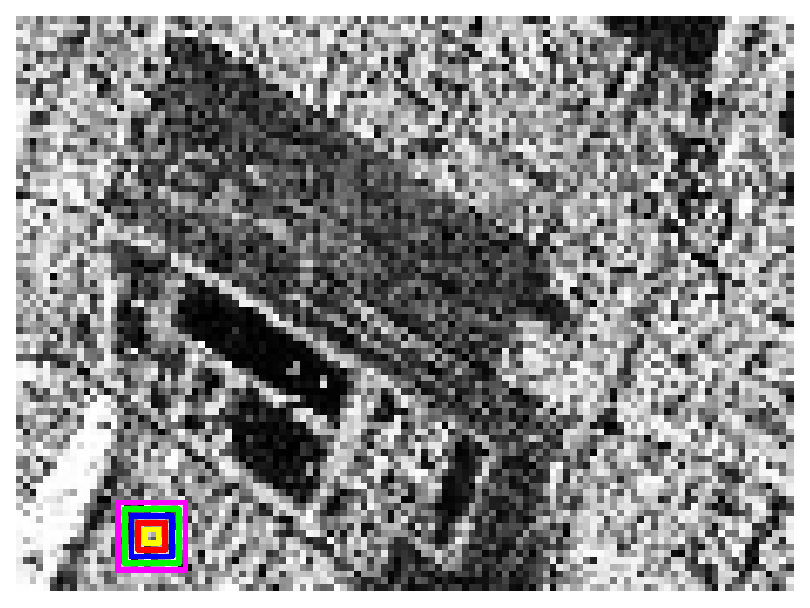
\includegraphics[width=0.7\linewidth]{../../../Figures/PaperTesis/CincoMuestras.eps}
	\caption{\label{CincoMuestras}\small Five sample used to compare $\widehat{\alpha}_{\text{{ML}}}$, $\widehat{\alpha}_{\Gamma}$, $\widehat{\alpha}_{\text{{LN}}}$ and  $\widehat{\alpha}_{\text{{LC}}}$.}
\end{figure}
\begin{figure}[htb]
	\centering
	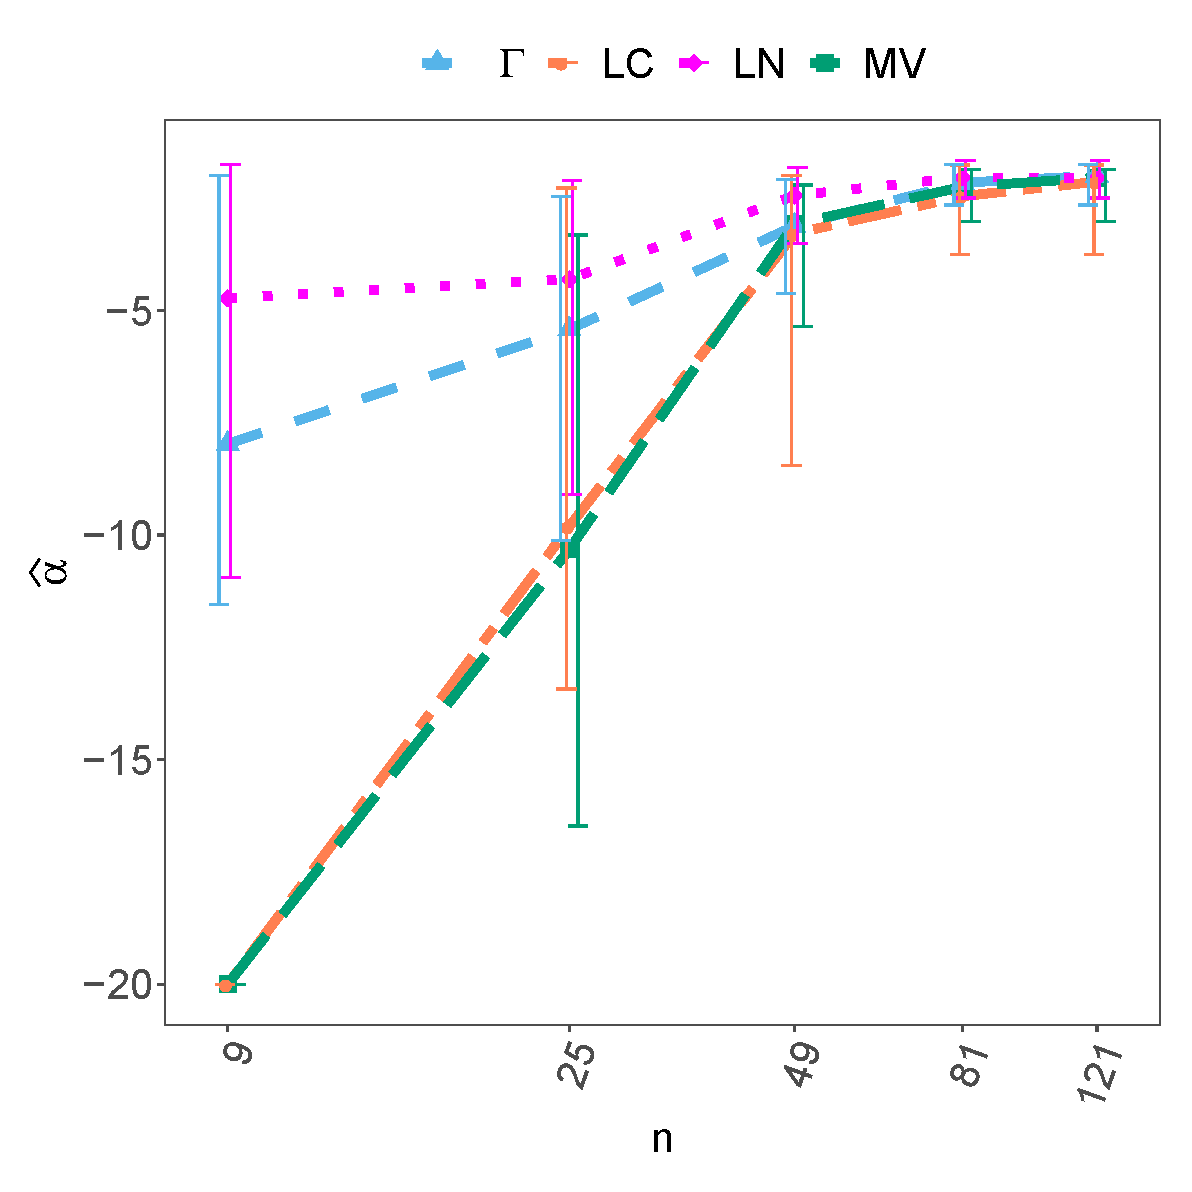
\includegraphics[width=0.7\linewidth]{../../../Figures/PaperTesis/AlfaVsTamCincoMuestras_v2.eps}
	\caption{\label{AlfaVsTamCincoMuestras}\small $\widehat{\alpha}_{\text{{ML}}}$, $\widehat{\alpha}_{\Gamma}$, $\widehat{\alpha}_{\text{{LN}}}$ and $\widehat{\alpha}_{\text{{LC}}}$ for corresponding samples to image~\ref{CincoMuestras}.}
\end{figure}

\begin{table}[hbt]
	\centering
	\caption{\label{TablaCincoMuestras} $\widehat{\alpha}$ for the samples correspond to image~\ref{CincoMuestras}.}
	\begin{tabular}{c*5{r}}
		\toprule
		Color       &  $n$    &  $\widehat{\alpha}_{\text{{ML}}}$    &  $\widehat{\alpha}_{\Gamma}$  &  $\widehat{\alpha}_{\text{{LN}}}$ &  $\widehat{\alpha}_{\text{{LC}}}$\\
		\midrule
		Yellow      & $9$     & $-20.00$      & $-7.97$ & $-4.73$ & $-20.00$\\
		Red         & $25$    & $-10.31$  & $-5.42$ & $-4.30$ & $-9.81$\\
		Blue        & $49$    & $-3.07$   & $-3.12$ & $-2.44$ & $-3.28$\\
		Green       & $81$    & $-2.24$   & $-2.15$ & $-2.03$ & $-2.45$\\
		Magenta     & $121$   & $-2.04$   & $-1.99$ & $-2.05$ & $-2.13$\\
		\bottomrule
	\end{tabular}
\end{table}


It can also be seen that the confidence intervals corresponding to the ML and LC methods are generally wider than those of the other methods. All intervals decrease in length as the sample size increases; that is, they become more precise. It is essential to mention that the confidence interval corresponding to the LN method is the one with presents the shortest length in most cases. It should be noted that, in the case where the ML and LC methods did not converge, there is no confidence interval and only the samples where all the methods converged were considered.

Figure~\ref{CornerReflector} shows the same ESAR image with a corner reflector. Several samples were chosen to estimate the $\alpha$ parameter. Some of these samples include the corner reflector.

\begin{figure}[htb]
	\centering
	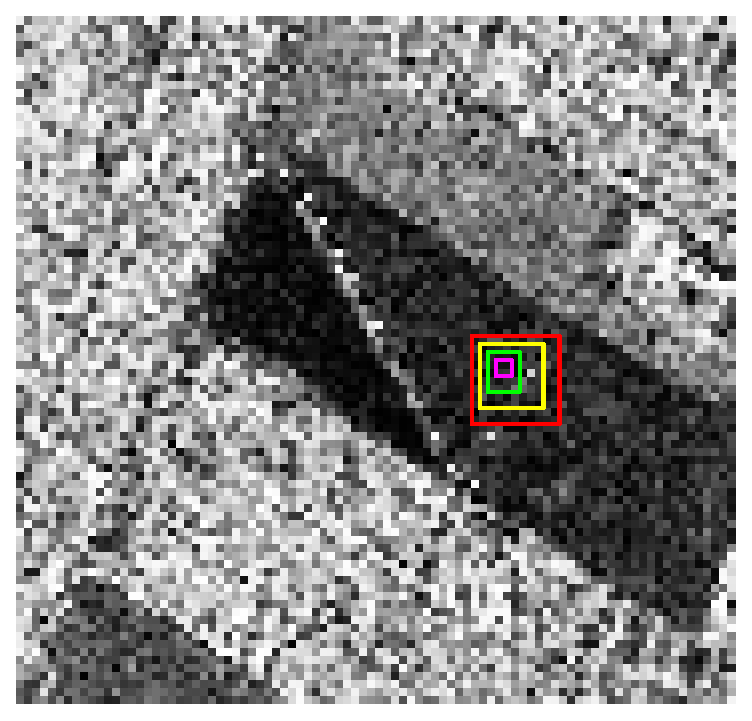
\includegraphics[width=0.7\linewidth]{../../../Figures/PaperTesis/CornerJulia_Roja.eps}
	\caption{\label{CornerReflector}\small $\widehat{\alpha}_{\text{{ML}}}$, $\widehat{\alpha}_{\Gamma}$, $\widehat{\alpha}_{\text{{LN}}}$ and $\widehat{\alpha}_{\text{{LC}}}$ with a corner reflector.}
\end{figure}

Table~\ref{ResultadosCorner} shows the estimation values. It can be seen that for $n=9$ none of the estimators converge. But for the rest of the sample size LN estimator shows greater stability. Even more the LN estimator does not show any change between the green sample and the yellow sample which contains the corner reflector. All the other method showed changes in the estimation by changing the type of texture from one sample to another. 

\begin{table}
	\label{ResultadosCorner} 
	\caption{$\widehat{\alpha}$ estimated values.}
	%\begin{tabular}{c 5*(c c c c c)}
	\begin{tabular}{c c S[table-number-alignment = right] S[table-number-alignment = right] S[table-number-alignment = right] S[table-number-alignment = right]}
		%\toprule
		Color & $n$ &  $\widehat\alpha_{\text{\tiny{MV}}}$ & $\widehat{\alpha_{\Gamma}}$ &$\widehat\alpha_{\text{{LN}}}$  &$\widehat\alpha_{\text{{LC}}}$ \\
		\midrule
		Magenta     & 9   & -20.00   & -20.00  & -20.00   & -20.00    \\
		Green       & 30  & -13.04  & -6.82  & \textcolor{red}{$-7.76$}     &  -20.00  \\
		Yellow     & 72   & -4.72  & -5.09   & \textcolor{red}{$-7.99$}     &  -4.29    \\
		Red        & 132  & -6.94  & -8.42   & \textcolor{red}{$-8.53$}     &   -6.79\\
		%\bottomrule
	\end{tabular}
\end{table}

\section{Conclusions}
\label{conclusion}

This work presents improvements to the MDE estimator for the texture parameter of the $\mathcal{G}^0$ model for intensity and multilook data, with respect to the one studied en~\cite{gambini2015}. We assess two other kernels: Lognormal and $\Gamma$, we use the LSCV method to obtain the bandwidth instead of using a fixed one empirically chosen, and we also implemented an optimization procedure to find the minimum, maximum and the roots of the functions associated with each of the estimators analyzed. 
The kernels were evaluated to estimate the underlying density function in terms of MISE and the percentage of non-convergence cases. 
We show that the IG kernel, together with fixed bandwidth as the one obtained by the LSCV, has higher MISE in all of the studied cases and a higher percentage of non-convergence cases in most of the instances analyzed with respect to the one presented by the $\Gamma$ and Lognormal kernels. For these reasons, we choose the latter to continue the analysis.

In the Monte Carlo study, it can be seen that: 
a)~On the one hand, the ML and LC methods have similar behavior to each other and, on the other, the MDE estimators using LN and $\Gamma$ kernels for both uncontaminated and contaminated data. Even this behavior occurs when analyzing the SEIF function.
b)~For uncontaminated and textured data, the MDE estimator is competitive with respect to the ML and LC in terms of bias and MSE. 
However, MDE outperforms ML and LC estimators in the presence of contamination, either using $\Gamma$ or LN kernels, and the latter is the one which presents the most stable behavior.
c)~The percentage of non-convergence cases presented by MDE estimators is significantly lower compared to the ML and LC estimators.
d)~The computational time of the MDE estimators is significantly larger than ML and LC estimators.

MDE, together with the Lognormal kernel showed the best performance in the application to actual data, exceeding ML and LC estimators. Based on the previous evidence, the MDE estimator has excellent properties measured by its bias, mean square error, and number of cases of non-convergence. 
It is competitive with the ML estimators and LC estimators in situations without contamination and exceeds these methods in the presence of small levels of contamination. It even showed better performance than the other estimators in the presence of a reflector corner.

For this reason, we conclude that it is advisable to use $\widehat{\alpha}_{\text{\tiny{T}}}$ with LN kernel, especially when using small samples and/or against the presence of contaminated data. 
Although the additional computational cost of the MDE estimator is not negligible, its advantages are more important than this increase in processing time.

All studies were made in the \texttt R platform and language for statistical computing~\cite{RLanguage}.


\bibliographystyle{spmpsci}
\bibliography{../../../Bibliography/bib_julia2}

%	\begin{IEEEbiography}[{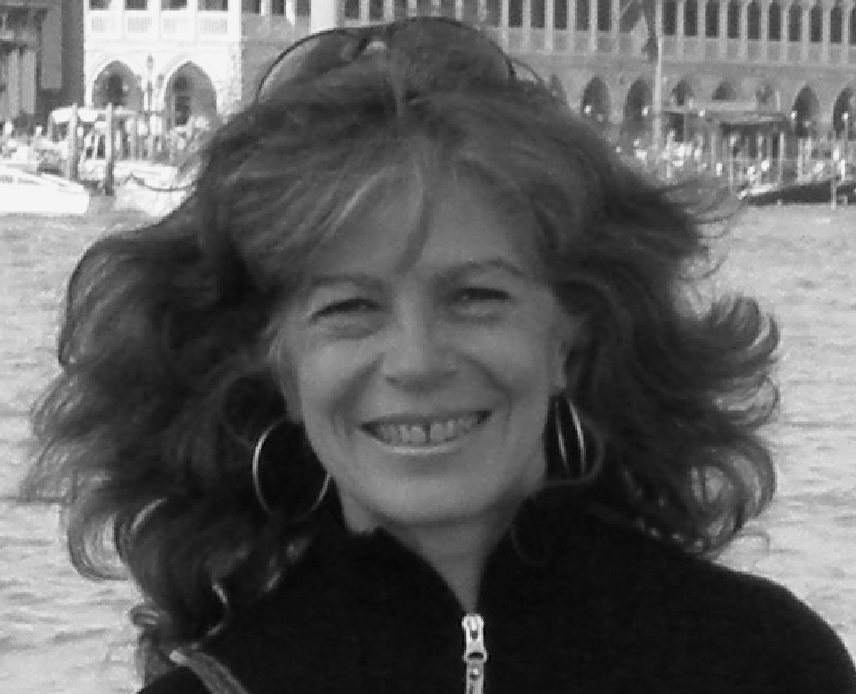
\includegraphics[height=1.2in,width=1.in]{../../../Images/Fotos/Cassetti_gray}}]{Julia Cassetti} 
%		received the B.Sc. degree in Mathematics and a postgraduate diploma in Mathematical Statistics, both from the Universidad de Buenos Aires (UBA), Argentina. 
%		She is currently an Assistant Professor at the Universidad Nacional de General Sarmiento, Argentina. 
%		Her research interests are SAR imaging and applied statistics.
%	\end{IEEEbiography}
%	
%	\vfill
%	
%	\begin{IEEEbiography}[{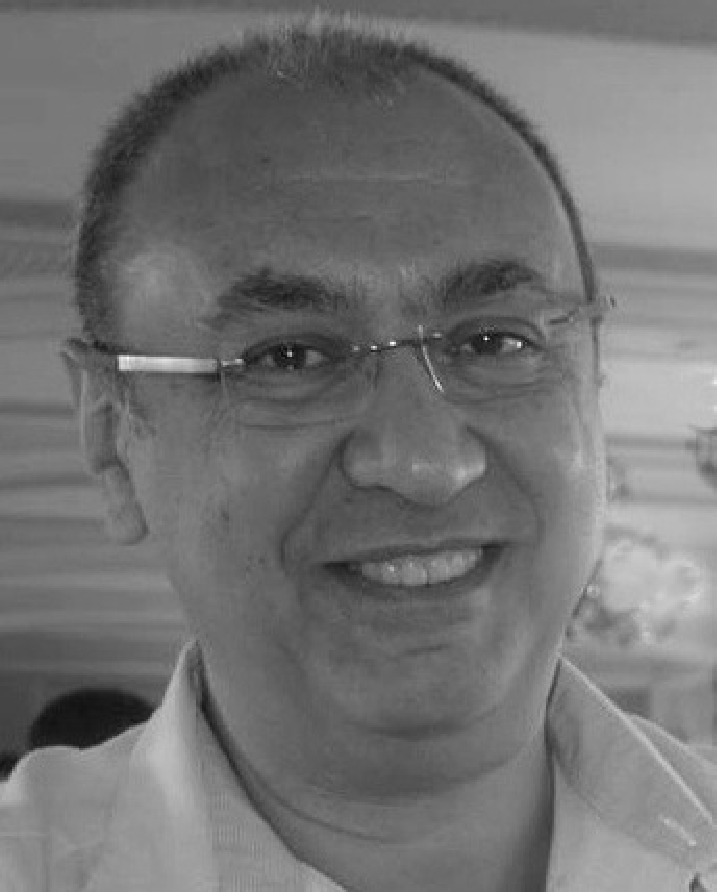
\includegraphics[width=1in]{../../../Images/Fotos/ACFrery_gray}}]{Alejandro C.\ Frery} (S'92--SM'03)
%		received the B.Sc. degree in Electronic and Electrical Engineering from the Universidad de Mendoza, Mendoza, Argentina.
%		His M.Sc. degree was in Applied Mathematics (Statistics) from the Instituto de Matem\'atica Pura e Aplicada (IMPA, Rio de Janeiro) and his Ph.D. degree was in Applied Computing from the Instituto Nacional de Pesquisas Espaciais (INPE, S\~ao Jos\'e dos Campos, Brazil).
%		He is currently the leader of LaCCAN -- \textit{Laborat\'orio de Computa\c c\~ao Cient\'ifica e An\'alise Num\'erica}, Universidade Federal de Alagoas, Macei\'o, Brazil.
%		His research interests are statistical computing and stochastic modelling.
%	\end{IEEEbiography}
\end{document}